
% Default to the notebook output style

    


% Inherit from the specified cell style.




    
\documentclass[11pt]{article}

    
    
    \usepackage[T1]{fontenc}
    % Nicer default font (+ math font) than Computer Modern for most use cases
    \usepackage{mathpazo}

    % Basic figure setup, for now with no caption control since it's done
    % automatically by Pandoc (which extracts ![](path) syntax from Markdown).
    \usepackage{graphicx}
    % We will generate all images so they have a width \maxwidth. This means
    % that they will get their normal width if they fit onto the page, but
    % are scaled down if they would overflow the margins.
    \makeatletter
    \def\maxwidth{\ifdim\Gin@nat@width>\linewidth\linewidth
    \else\Gin@nat@width\fi}
    \makeatother
    \let\Oldincludegraphics\includegraphics
    % Set max figure width to be 80% of text width, for now hardcoded.
    \renewcommand{\includegraphics}[1]{\Oldincludegraphics[width=.8\maxwidth]{#1}}
    % Ensure that by default, figures have no caption (until we provide a
    % proper Figure object with a Caption API and a way to capture that
    % in the conversion process - todo).
    \usepackage{caption}
    \DeclareCaptionLabelFormat{nolabel}{}
    \captionsetup{labelformat=nolabel}

    \usepackage{adjustbox} % Used to constrain images to a maximum size 
    \usepackage{xcolor} % Allow colors to be defined
    \usepackage{enumerate} % Needed for markdown enumerations to work
    \usepackage{geometry} % Used to adjust the document margins
    \usepackage{amsmath} % Equations
    \usepackage{amssymb} % Equations
    \usepackage{textcomp} % defines textquotesingle
    % Hack from http://tex.stackexchange.com/a/47451/13684:
    \AtBeginDocument{%
        \def\PYZsq{\textquotesingle}% Upright quotes in Pygmentized code
    }
    \usepackage{upquote} % Upright quotes for verbatim code
    \usepackage{eurosym} % defines \euro
    \usepackage[mathletters]{ucs} % Extended unicode (utf-8) support
    \usepackage[utf8x]{inputenc} % Allow utf-8 characters in the tex document
    \usepackage{fancyvrb} % verbatim replacement that allows latex
    \usepackage{grffile} % extends the file name processing of package graphics 
                         % to support a larger range 
    % The hyperref package gives us a pdf with properly built
    % internal navigation ('pdf bookmarks' for the table of contents,
    % internal cross-reference links, web links for URLs, etc.)
    \usepackage{hyperref}
    \usepackage{longtable} % longtable support required by pandoc >1.10
    \usepackage{booktabs}  % table support for pandoc > 1.12.2
    \usepackage[inline]{enumitem} % IRkernel/repr support (it uses the enumerate* environment)
    \usepackage[normalem]{ulem} % ulem is needed to support strikethroughs (\sout)
                                % normalem makes italics be italics, not underlines
    \usepackage{mathrsfs}
    

    
    
    % Colors for the hyperref package
    \definecolor{urlcolor}{rgb}{0,.145,.698}
    \definecolor{linkcolor}{rgb}{.71,0.21,0.01}
    \definecolor{citecolor}{rgb}{.12,.54,.11}

    % ANSI colors
    \definecolor{ansi-black}{HTML}{3E424D}
    \definecolor{ansi-black-intense}{HTML}{282C36}
    \definecolor{ansi-red}{HTML}{E75C58}
    \definecolor{ansi-red-intense}{HTML}{B22B31}
    \definecolor{ansi-green}{HTML}{00A250}
    \definecolor{ansi-green-intense}{HTML}{007427}
    \definecolor{ansi-yellow}{HTML}{DDB62B}
    \definecolor{ansi-yellow-intense}{HTML}{B27D12}
    \definecolor{ansi-blue}{HTML}{208FFB}
    \definecolor{ansi-blue-intense}{HTML}{0065CA}
    \definecolor{ansi-magenta}{HTML}{D160C4}
    \definecolor{ansi-magenta-intense}{HTML}{A03196}
    \definecolor{ansi-cyan}{HTML}{60C6C8}
    \definecolor{ansi-cyan-intense}{HTML}{258F8F}
    \definecolor{ansi-white}{HTML}{C5C1B4}
    \definecolor{ansi-white-intense}{HTML}{A1A6B2}
    \definecolor{ansi-default-inverse-fg}{HTML}{FFFFFF}
    \definecolor{ansi-default-inverse-bg}{HTML}{000000}

    % commands and environments needed by pandoc snippets
    % extracted from the output of `pandoc -s`
    \providecommand{\tightlist}{%
      \setlength{\itemsep}{0pt}\setlength{\parskip}{0pt}}
    \DefineVerbatimEnvironment{Highlighting}{Verbatim}{commandchars=\\\{\}}
    % Add ',fontsize=\small' for more characters per line
    \newenvironment{Shaded}{}{}
    \newcommand{\KeywordTok}[1]{\textcolor[rgb]{0.00,0.44,0.13}{\textbf{{#1}}}}
    \newcommand{\DataTypeTok}[1]{\textcolor[rgb]{0.56,0.13,0.00}{{#1}}}
    \newcommand{\DecValTok}[1]{\textcolor[rgb]{0.25,0.63,0.44}{{#1}}}
    \newcommand{\BaseNTok}[1]{\textcolor[rgb]{0.25,0.63,0.44}{{#1}}}
    \newcommand{\FloatTok}[1]{\textcolor[rgb]{0.25,0.63,0.44}{{#1}}}
    \newcommand{\CharTok}[1]{\textcolor[rgb]{0.25,0.44,0.63}{{#1}}}
    \newcommand{\StringTok}[1]{\textcolor[rgb]{0.25,0.44,0.63}{{#1}}}
    \newcommand{\CommentTok}[1]{\textcolor[rgb]{0.38,0.63,0.69}{\textit{{#1}}}}
    \newcommand{\OtherTok}[1]{\textcolor[rgb]{0.00,0.44,0.13}{{#1}}}
    \newcommand{\AlertTok}[1]{\textcolor[rgb]{1.00,0.00,0.00}{\textbf{{#1}}}}
    \newcommand{\FunctionTok}[1]{\textcolor[rgb]{0.02,0.16,0.49}{{#1}}}
    \newcommand{\RegionMarkerTok}[1]{{#1}}
    \newcommand{\ErrorTok}[1]{\textcolor[rgb]{1.00,0.00,0.00}{\textbf{{#1}}}}
    \newcommand{\NormalTok}[1]{{#1}}
    
    % Additional commands for more recent versions of Pandoc
    \newcommand{\ConstantTok}[1]{\textcolor[rgb]{0.53,0.00,0.00}{{#1}}}
    \newcommand{\SpecialCharTok}[1]{\textcolor[rgb]{0.25,0.44,0.63}{{#1}}}
    \newcommand{\VerbatimStringTok}[1]{\textcolor[rgb]{0.25,0.44,0.63}{{#1}}}
    \newcommand{\SpecialStringTok}[1]{\textcolor[rgb]{0.73,0.40,0.53}{{#1}}}
    \newcommand{\ImportTok}[1]{{#1}}
    \newcommand{\DocumentationTok}[1]{\textcolor[rgb]{0.73,0.13,0.13}{\textit{{#1}}}}
    \newcommand{\AnnotationTok}[1]{\textcolor[rgb]{0.38,0.63,0.69}{\textbf{\textit{{#1}}}}}
    \newcommand{\CommentVarTok}[1]{\textcolor[rgb]{0.38,0.63,0.69}{\textbf{\textit{{#1}}}}}
    \newcommand{\VariableTok}[1]{\textcolor[rgb]{0.10,0.09,0.49}{{#1}}}
    \newcommand{\ControlFlowTok}[1]{\textcolor[rgb]{0.00,0.44,0.13}{\textbf{{#1}}}}
    \newcommand{\OperatorTok}[1]{\textcolor[rgb]{0.40,0.40,0.40}{{#1}}}
    \newcommand{\BuiltInTok}[1]{{#1}}
    \newcommand{\ExtensionTok}[1]{{#1}}
    \newcommand{\PreprocessorTok}[1]{\textcolor[rgb]{0.74,0.48,0.00}{{#1}}}
    \newcommand{\AttributeTok}[1]{\textcolor[rgb]{0.49,0.56,0.16}{{#1}}}
    \newcommand{\InformationTok}[1]{\textcolor[rgb]{0.38,0.63,0.69}{\textbf{\textit{{#1}}}}}
    \newcommand{\WarningTok}[1]{\textcolor[rgb]{0.38,0.63,0.69}{\textbf{\textit{{#1}}}}}
    
    
    % Define a nice break command that doesn't care if a line doesn't already
    % exist.
    \def\br{\hspace*{\fill} \\* }
    % Math Jax compatibility definitions
    \def\gt{>}
    \def\lt{<}
    \let\Oldtex\TeX
    \let\Oldlatex\LaTeX
    \renewcommand{\TeX}{\textrm{\Oldtex}}
    \renewcommand{\LaTeX}{\textrm{\Oldlatex}}
    % Document parameters
    % Document title
    \title{CarterKaoLetcherPhilippou\_w261\_FM\_CTR}
    
    
    
    
    

    % Pygments definitions
    
\makeatletter
\def\PY@reset{\let\PY@it=\relax \let\PY@bf=\relax%
    \let\PY@ul=\relax \let\PY@tc=\relax%
    \let\PY@bc=\relax \let\PY@ff=\relax}
\def\PY@tok#1{\csname PY@tok@#1\endcsname}
\def\PY@toks#1+{\ifx\relax#1\empty\else%
    \PY@tok{#1}\expandafter\PY@toks\fi}
\def\PY@do#1{\PY@bc{\PY@tc{\PY@ul{%
    \PY@it{\PY@bf{\PY@ff{#1}}}}}}}
\def\PY#1#2{\PY@reset\PY@toks#1+\relax+\PY@do{#2}}

\expandafter\def\csname PY@tok@w\endcsname{\def\PY@tc##1{\textcolor[rgb]{0.73,0.73,0.73}{##1}}}
\expandafter\def\csname PY@tok@c\endcsname{\let\PY@it=\textit\def\PY@tc##1{\textcolor[rgb]{0.25,0.50,0.50}{##1}}}
\expandafter\def\csname PY@tok@cp\endcsname{\def\PY@tc##1{\textcolor[rgb]{0.74,0.48,0.00}{##1}}}
\expandafter\def\csname PY@tok@k\endcsname{\let\PY@bf=\textbf\def\PY@tc##1{\textcolor[rgb]{0.00,0.50,0.00}{##1}}}
\expandafter\def\csname PY@tok@kp\endcsname{\def\PY@tc##1{\textcolor[rgb]{0.00,0.50,0.00}{##1}}}
\expandafter\def\csname PY@tok@kt\endcsname{\def\PY@tc##1{\textcolor[rgb]{0.69,0.00,0.25}{##1}}}
\expandafter\def\csname PY@tok@o\endcsname{\def\PY@tc##1{\textcolor[rgb]{0.40,0.40,0.40}{##1}}}
\expandafter\def\csname PY@tok@ow\endcsname{\let\PY@bf=\textbf\def\PY@tc##1{\textcolor[rgb]{0.67,0.13,1.00}{##1}}}
\expandafter\def\csname PY@tok@nb\endcsname{\def\PY@tc##1{\textcolor[rgb]{0.00,0.50,0.00}{##1}}}
\expandafter\def\csname PY@tok@nf\endcsname{\def\PY@tc##1{\textcolor[rgb]{0.00,0.00,1.00}{##1}}}
\expandafter\def\csname PY@tok@nc\endcsname{\let\PY@bf=\textbf\def\PY@tc##1{\textcolor[rgb]{0.00,0.00,1.00}{##1}}}
\expandafter\def\csname PY@tok@nn\endcsname{\let\PY@bf=\textbf\def\PY@tc##1{\textcolor[rgb]{0.00,0.00,1.00}{##1}}}
\expandafter\def\csname PY@tok@ne\endcsname{\let\PY@bf=\textbf\def\PY@tc##1{\textcolor[rgb]{0.82,0.25,0.23}{##1}}}
\expandafter\def\csname PY@tok@nv\endcsname{\def\PY@tc##1{\textcolor[rgb]{0.10,0.09,0.49}{##1}}}
\expandafter\def\csname PY@tok@no\endcsname{\def\PY@tc##1{\textcolor[rgb]{0.53,0.00,0.00}{##1}}}
\expandafter\def\csname PY@tok@nl\endcsname{\def\PY@tc##1{\textcolor[rgb]{0.63,0.63,0.00}{##1}}}
\expandafter\def\csname PY@tok@ni\endcsname{\let\PY@bf=\textbf\def\PY@tc##1{\textcolor[rgb]{0.60,0.60,0.60}{##1}}}
\expandafter\def\csname PY@tok@na\endcsname{\def\PY@tc##1{\textcolor[rgb]{0.49,0.56,0.16}{##1}}}
\expandafter\def\csname PY@tok@nt\endcsname{\let\PY@bf=\textbf\def\PY@tc##1{\textcolor[rgb]{0.00,0.50,0.00}{##1}}}
\expandafter\def\csname PY@tok@nd\endcsname{\def\PY@tc##1{\textcolor[rgb]{0.67,0.13,1.00}{##1}}}
\expandafter\def\csname PY@tok@s\endcsname{\def\PY@tc##1{\textcolor[rgb]{0.73,0.13,0.13}{##1}}}
\expandafter\def\csname PY@tok@sd\endcsname{\let\PY@it=\textit\def\PY@tc##1{\textcolor[rgb]{0.73,0.13,0.13}{##1}}}
\expandafter\def\csname PY@tok@si\endcsname{\let\PY@bf=\textbf\def\PY@tc##1{\textcolor[rgb]{0.73,0.40,0.53}{##1}}}
\expandafter\def\csname PY@tok@se\endcsname{\let\PY@bf=\textbf\def\PY@tc##1{\textcolor[rgb]{0.73,0.40,0.13}{##1}}}
\expandafter\def\csname PY@tok@sr\endcsname{\def\PY@tc##1{\textcolor[rgb]{0.73,0.40,0.53}{##1}}}
\expandafter\def\csname PY@tok@ss\endcsname{\def\PY@tc##1{\textcolor[rgb]{0.10,0.09,0.49}{##1}}}
\expandafter\def\csname PY@tok@sx\endcsname{\def\PY@tc##1{\textcolor[rgb]{0.00,0.50,0.00}{##1}}}
\expandafter\def\csname PY@tok@m\endcsname{\def\PY@tc##1{\textcolor[rgb]{0.40,0.40,0.40}{##1}}}
\expandafter\def\csname PY@tok@gh\endcsname{\let\PY@bf=\textbf\def\PY@tc##1{\textcolor[rgb]{0.00,0.00,0.50}{##1}}}
\expandafter\def\csname PY@tok@gu\endcsname{\let\PY@bf=\textbf\def\PY@tc##1{\textcolor[rgb]{0.50,0.00,0.50}{##1}}}
\expandafter\def\csname PY@tok@gd\endcsname{\def\PY@tc##1{\textcolor[rgb]{0.63,0.00,0.00}{##1}}}
\expandafter\def\csname PY@tok@gi\endcsname{\def\PY@tc##1{\textcolor[rgb]{0.00,0.63,0.00}{##1}}}
\expandafter\def\csname PY@tok@gr\endcsname{\def\PY@tc##1{\textcolor[rgb]{1.00,0.00,0.00}{##1}}}
\expandafter\def\csname PY@tok@ge\endcsname{\let\PY@it=\textit}
\expandafter\def\csname PY@tok@gs\endcsname{\let\PY@bf=\textbf}
\expandafter\def\csname PY@tok@gp\endcsname{\let\PY@bf=\textbf\def\PY@tc##1{\textcolor[rgb]{0.00,0.00,0.50}{##1}}}
\expandafter\def\csname PY@tok@go\endcsname{\def\PY@tc##1{\textcolor[rgb]{0.53,0.53,0.53}{##1}}}
\expandafter\def\csname PY@tok@gt\endcsname{\def\PY@tc##1{\textcolor[rgb]{0.00,0.27,0.87}{##1}}}
\expandafter\def\csname PY@tok@err\endcsname{\def\PY@bc##1{\setlength{\fboxsep}{0pt}\fcolorbox[rgb]{1.00,0.00,0.00}{1,1,1}{\strut ##1}}}
\expandafter\def\csname PY@tok@kc\endcsname{\let\PY@bf=\textbf\def\PY@tc##1{\textcolor[rgb]{0.00,0.50,0.00}{##1}}}
\expandafter\def\csname PY@tok@kd\endcsname{\let\PY@bf=\textbf\def\PY@tc##1{\textcolor[rgb]{0.00,0.50,0.00}{##1}}}
\expandafter\def\csname PY@tok@kn\endcsname{\let\PY@bf=\textbf\def\PY@tc##1{\textcolor[rgb]{0.00,0.50,0.00}{##1}}}
\expandafter\def\csname PY@tok@kr\endcsname{\let\PY@bf=\textbf\def\PY@tc##1{\textcolor[rgb]{0.00,0.50,0.00}{##1}}}
\expandafter\def\csname PY@tok@bp\endcsname{\def\PY@tc##1{\textcolor[rgb]{0.00,0.50,0.00}{##1}}}
\expandafter\def\csname PY@tok@fm\endcsname{\def\PY@tc##1{\textcolor[rgb]{0.00,0.00,1.00}{##1}}}
\expandafter\def\csname PY@tok@vc\endcsname{\def\PY@tc##1{\textcolor[rgb]{0.10,0.09,0.49}{##1}}}
\expandafter\def\csname PY@tok@vg\endcsname{\def\PY@tc##1{\textcolor[rgb]{0.10,0.09,0.49}{##1}}}
\expandafter\def\csname PY@tok@vi\endcsname{\def\PY@tc##1{\textcolor[rgb]{0.10,0.09,0.49}{##1}}}
\expandafter\def\csname PY@tok@vm\endcsname{\def\PY@tc##1{\textcolor[rgb]{0.10,0.09,0.49}{##1}}}
\expandafter\def\csname PY@tok@sa\endcsname{\def\PY@tc##1{\textcolor[rgb]{0.73,0.13,0.13}{##1}}}
\expandafter\def\csname PY@tok@sb\endcsname{\def\PY@tc##1{\textcolor[rgb]{0.73,0.13,0.13}{##1}}}
\expandafter\def\csname PY@tok@sc\endcsname{\def\PY@tc##1{\textcolor[rgb]{0.73,0.13,0.13}{##1}}}
\expandafter\def\csname PY@tok@dl\endcsname{\def\PY@tc##1{\textcolor[rgb]{0.73,0.13,0.13}{##1}}}
\expandafter\def\csname PY@tok@s2\endcsname{\def\PY@tc##1{\textcolor[rgb]{0.73,0.13,0.13}{##1}}}
\expandafter\def\csname PY@tok@sh\endcsname{\def\PY@tc##1{\textcolor[rgb]{0.73,0.13,0.13}{##1}}}
\expandafter\def\csname PY@tok@s1\endcsname{\def\PY@tc##1{\textcolor[rgb]{0.73,0.13,0.13}{##1}}}
\expandafter\def\csname PY@tok@mb\endcsname{\def\PY@tc##1{\textcolor[rgb]{0.40,0.40,0.40}{##1}}}
\expandafter\def\csname PY@tok@mf\endcsname{\def\PY@tc##1{\textcolor[rgb]{0.40,0.40,0.40}{##1}}}
\expandafter\def\csname PY@tok@mh\endcsname{\def\PY@tc##1{\textcolor[rgb]{0.40,0.40,0.40}{##1}}}
\expandafter\def\csname PY@tok@mi\endcsname{\def\PY@tc##1{\textcolor[rgb]{0.40,0.40,0.40}{##1}}}
\expandafter\def\csname PY@tok@il\endcsname{\def\PY@tc##1{\textcolor[rgb]{0.40,0.40,0.40}{##1}}}
\expandafter\def\csname PY@tok@mo\endcsname{\def\PY@tc##1{\textcolor[rgb]{0.40,0.40,0.40}{##1}}}
\expandafter\def\csname PY@tok@ch\endcsname{\let\PY@it=\textit\def\PY@tc##1{\textcolor[rgb]{0.25,0.50,0.50}{##1}}}
\expandafter\def\csname PY@tok@cm\endcsname{\let\PY@it=\textit\def\PY@tc##1{\textcolor[rgb]{0.25,0.50,0.50}{##1}}}
\expandafter\def\csname PY@tok@cpf\endcsname{\let\PY@it=\textit\def\PY@tc##1{\textcolor[rgb]{0.25,0.50,0.50}{##1}}}
\expandafter\def\csname PY@tok@c1\endcsname{\let\PY@it=\textit\def\PY@tc##1{\textcolor[rgb]{0.25,0.50,0.50}{##1}}}
\expandafter\def\csname PY@tok@cs\endcsname{\let\PY@it=\textit\def\PY@tc##1{\textcolor[rgb]{0.25,0.50,0.50}{##1}}}

\def\PYZbs{\char`\\}
\def\PYZus{\char`\_}
\def\PYZob{\char`\{}
\def\PYZcb{\char`\}}
\def\PYZca{\char`\^}
\def\PYZam{\char`\&}
\def\PYZlt{\char`\<}
\def\PYZgt{\char`\>}
\def\PYZsh{\char`\#}
\def\PYZpc{\char`\%}
\def\PYZdl{\char`\$}
\def\PYZhy{\char`\-}
\def\PYZsq{\char`\'}
\def\PYZdq{\char`\"}
\def\PYZti{\char`\~}
% for compatibility with earlier versions
\def\PYZat{@}
\def\PYZlb{[}
\def\PYZrb{]}
\makeatother


    % Exact colors from NB
    \definecolor{incolor}{rgb}{0.0, 0.0, 0.5}
    \definecolor{outcolor}{rgb}{0.545, 0.0, 0.0}



    
    % Prevent overflowing lines due to hard-to-break entities
    \sloppy 
    % Setup hyperref package
    \hypersetup{
      breaklinks=true,  % so long urls are correctly broken across lines
      colorlinks=true,
      urlcolor=urlcolor,
      linkcolor=linkcolor,
      citecolor=citecolor,
      }
    % Slightly bigger margins than the latex defaults
    
    \geometry{verbose,tmargin=1in,bmargin=1in,lmargin=1in,rmargin=1in}
    
    

    \begin{document}
    
    
    \maketitle
    
    

    
    \section{Click Through Rate (CTR) Prediction using Factorization
Machines at
Scale}\label{click-through-rate-ctr-prediction-using-factorization-machines-at-scale}

\subsection{MIDS w261 Final Project}\label{mids-w261-final-project}

\subsection{December 12, 2018}\label{december-12-2018}

\textbf{Authors}: Colby Carter, Kalvin Kao, Adam Letcher, Jennifer
Philippou

    

    \section{1. Project Purpose}\label{project-purpose}

\subsubsection{\texorpdfstring{\emph{Introduction}}{Introduction}}\label{introduction}

Since the explosion of global internet usage, the advertising industry
has adapted to utilize the internet to entice users to purchase their
products, subscribe to their services, or generally perceive their brand
in a positive light. Display advertising is a form of advertising on
third party sites (such as social networks) or search engines that allow
companies to market directly to consumers. This industry has grown
rapidly with the adoption of internet usage in homes and on mobile
devices worldwide, and a key metric in determining the effectiveness of
such marketing campaigns is a "click through rate". Naturally, given the
huge financial incentives, models which are able to identify important
drivers of click through rates, or even predict the click through rate
of a campaign, are highly desirable.

The Criteo Labs display ad challenge was a machine learning competition
hosted on Kaggle that provided a week's worth of data to participants
and asked them to build a predictive model that would answer the
question "Given a user and the page they are visiting, what is the
probability that they will click on a given ad?". The competition was
scored by calculating a log-loss for submitted predictions based on a
held-out test dataset. While the challenge concluded in 2014, this
project will use the same dataset and scoring to demonstrate a scalable
machine learning model that is capable of handling the large amount of
Criteo data efficiently by using Apache Spark running on Google's cloud
engine.

https://www.kaggle.com/c/criteo-display-ad-challenge

\subsubsection{\texorpdfstring{\emph{Data
Description}}{Data Description}}\label{data-description}

The training dataset consists of a portion of Criteo's traffic over a
period of 7 days. Each row corresponds to a display ad served by Criteo.
Positive (clicked) and negatives (non-clicked) examples have both been
subsampled at different rates in order to reduce the dataset size.
Downloading the dataset requires signing a user agreement so it was not
an automated step (link provided below). The datafields consist of the
following:

\begin{itemize}
\tightlist
\item
  Label - Target variable that indicates if an ad was clicked (1) or not
  (0).
\item
  I1-I13 - A total of 13 columns of integer features (mostly count
  features).
\item
  C1-C26 - A total of 26 columns of categorical features. The values of
  these features have been hashed onto 32 bits for anonymization
  purposes.
\end{itemize}

The total training dataset consists of approximately 46 million records.
There are a large number of categorical features which require a one-hot
encoding approach (which will be discussed further in later sections),
which result in a transformed dataset with approximately 35 million
unique features, with only an average of 48 non-zero entries per record.
This is a large, sparse dataset that will require special treatment in
order to efficiently handle and take advantage of Spark's ability to
process data in parallel and in memory (primarily). Additionally, in
order to be useful from a practical point of view, the methodologies for
modeling based on these data need to continue to be scalable far beyond
just the seven day snapshot provided for the challenge, and lightweight
enough to make predictions on future display ads in a timeframe that
supports the ultimate business objectives.

http://labs.criteo.com/2014/09/kaggle-contest-dataset-now-available-academic-use/

\subsubsection{\texorpdfstring{\emph{Project
Outline}}{Project Outline}}\label{project-outline}

In the remainder of this report, we will walk through an explanation of
our chosen algorithmic approach using a toy example, provide an
exploratory data analysis (EDA) using a sample of the full dataset, and
then describe our implementation of the algorithm at scale. Finally, we
will discuss the practical concepts of scalability utilized in our
approach, highlight any challenges that arose during the course of the
project, and identify any future exploration or modifications that could
be made to our approach in order to improve its predictive power or
training performance.

    \section{2. Factorization Machines}\label{factorization-machines}

For this project, our team chose to take an approach that utilized
Factorization Machines (FM), similar to other successful challenge
participants. FMs are a model class that combine the advantages of
matrix factorization models with Support Vector Machines (SVM). FMs are
a general predictor that work with any real valued feature vector, but
they improve on SVMs by modeling all interaction terms between variables
using factorized variables. This allows FMs to model complex
interactions even in situations with a large amount of sparsity, such as
this particular dataset (described above). Additionally, as shown in the
original paper by Rendle, FMs can be calculated in linear time through a
reformulation of the model equation, making them very attractive in
terms of a scalable solution.

https://www.csie.ntu.edu.tw/\textasciitilde{}b97053/paper/Rendle2010FM.pdf

https://www.csie.ntu.edu.tw/\textasciitilde{}r01922136/slides/ffm.pdf

The model equation for an FM of degree equal to two is shown in the
image below. As described in the original Rendle paper, a 2-way FM
models all single and pairwise iteractions between features where:

\begin{itemize}
\tightlist
\item
  \(w_0\) represents the global bias
\item
  \(w_i\) represents the strength of the inidividual feature \(i\)
\item
  \(<v_i,v_j>\) represents the interaction between the \(i\)-th and
  \(j\)-th features
\end{itemize}

    \begin{figure}
\centering
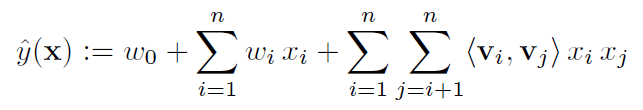
\includegraphics{FINAL/images/FM_equation_Rendle2010.png}
\caption{FM Equation}
\end{figure}

    The key difference between the FM model and a general polynomial model
is the third term, which models the interactions as the dot product of
two weights, rather than an individual weight \(w_i,j\). This
factorization means that no model parameter depends on any two variables
and therefore can be reformulated to an equation that has complexity
\(O(k\cdot n)\) instead of \(O(n^2)\). The image below shows the right
hand summands, which have been rewritten as the average of differences
between dot products for each factor \(k\):

    \begin{figure}
\centering
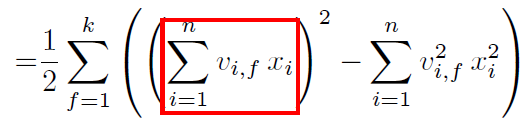
\includegraphics{FINAL/images/FM_factor_Rendle2010.png}
\caption{FM factor}
\end{figure}

    This closed form equation can be solved in linear time, and therefore
can be learned efficiently using forms of Gradient Descent. In later
sections of this document, we will describe our implementation of
gradient descent to learn a 2-way FM model. However, first we will
proceed with a toy problem to illustrate the mathematical description of
FMs above in a practical (although simple) setting.

    \subsection{Toy Example}\label{toy-example}

    Our team will use the toy data below to try and demonstrate the logic
and flow of the FM approach, where the data is a set of observations in
tab separated rows. In each row, the first value is a binary label where
1 represents a positive click-through and 0 represents no click-through.
The remaining values are the numeric and categorical features associated
with each record, which must be parses and stored in a tuple of (label,
features).

    \begin{Verbatim}[commandchars=\\\{\}]
{\color{incolor}In [{\color{incolor}10}]:} \PY{k+kn}{import} \PY{n+nn}{numpy} \PY{k}{as} \PY{n+nn}{np}
         
         \PY{n}{toyDataRaw} \PY{o}{=} \PY{p}{[}\PY{l+s+s1}{\PYZsq{}}\PY{l+s+s1}{1}\PY{l+s+se}{\PYZbs{}t}\PY{l+s+s1}{0}\PY{l+s+se}{\PYZbs{}t}\PY{l+s+s1}{5}\PY{l+s+se}{\PYZbs{}t}\PY{l+s+se}{\PYZbs{}t}\PY{l+s+s1}{1}\PY{l+s+se}{\PYZbs{}t}\PY{l+s+s1}{26}\PY{l+s+se}{\PYZbs{}t}\PY{l+s+s1}{cat}\PY{l+s+se}{\PYZbs{}t}\PY{l+s+s1}{blue}\PY{l+s+se}{\PYZbs{}t}\PY{l+s+se}{\PYZbs{}t}\PY{l+s+s1}{pizza}\PY{l+s+s1}{\PYZsq{}}\PY{p}{,}
                     \PY{l+s+s1}{\PYZsq{}}\PY{l+s+s1}{0}\PY{l+s+se}{\PYZbs{}t}\PY{l+s+s1}{1}\PY{l+s+se}{\PYZbs{}t}\PY{l+s+s1}{10}\PY{l+s+se}{\PYZbs{}t}\PY{l+s+s1}{1}\PY{l+s+se}{\PYZbs{}t}\PY{l+s+se}{\PYZbs{}t}\PY{l+s+s1}{12}\PY{l+s+se}{\PYZbs{}t}\PY{l+s+s1}{dog}\PY{l+s+se}{\PYZbs{}t}\PY{l+s+s1}{yellow}\PY{l+s+se}{\PYZbs{}t}\PY{l+s+se}{\PYZbs{}t}\PY{l+s+s1}{\PYZsq{}}\PY{p}{,}
                     \PY{l+s+s1}{\PYZsq{}}\PY{l+s+s1}{0}\PY{l+s+se}{\PYZbs{}t}\PY{l+s+s1}{0}\PY{l+s+se}{\PYZbs{}t}\PY{l+s+se}{\PYZbs{}t}\PY{l+s+s1}{0.5}\PY{l+s+se}{\PYZbs{}t}\PY{l+s+s1}{2}\PY{l+s+se}{\PYZbs{}t}\PY{l+s+s1}{45}\PY{l+s+se}{\PYZbs{}t}\PY{l+s+s1}{dog}\PY{l+s+se}{\PYZbs{}t}\PY{l+s+se}{\PYZbs{}t}\PY{l+s+s1}{car}\PY{l+s+se}{\PYZbs{}t}\PY{l+s+s1}{steak}\PY{l+s+s1}{\PYZsq{}}\PY{p}{]}
\end{Verbatim}

    \begin{Verbatim}[commandchars=\\\{\}]
{\color{incolor}In [{\color{incolor}11}]:} \PY{c+c1}{\PYZsh{} parse out label and features}
         \PY{n}{toyDataParsed} \PY{o}{=} \PY{p}{[}\PY{p}{]}
         \PY{k}{for} \PY{n}{row} \PY{o+ow}{in} \PY{n}{toyDataRaw}\PY{p}{:}
             \PY{n}{splitRow} \PY{o}{=} \PY{n}{row}\PY{o}{.}\PY{n}{split}\PY{p}{(}\PY{l+s+s1}{\PYZsq{}}\PY{l+s+se}{\PYZbs{}t}\PY{l+s+s1}{\PYZsq{}}\PY{p}{)}
             \PY{n}{toyDataParsed}\PY{o}{.}\PY{n}{append}\PY{p}{(}\PY{p}{(}\PY{n}{splitRow}\PY{p}{[}\PY{l+m+mi}{0}\PY{p}{]}\PY{p}{,} \PY{n}{splitRow}\PY{p}{[}\PY{l+m+mi}{1}\PY{p}{:}\PY{p}{]}\PY{p}{)}\PY{p}{)}
             
         \PY{n+nb}{print}\PY{p}{(}\PY{l+s+s2}{\PYZdq{}}\PY{l+s+s2}{Toy data made up of label followed by numeric and categorical features:}\PY{l+s+s2}{\PYZdq{}}\PY{p}{)}
         \PY{n}{toyDataParsed}
\end{Verbatim}

    \begin{Verbatim}[commandchars=\\\{\}]
Toy data made up of label followed by numeric and categorical features:

    \end{Verbatim}

\begin{Verbatim}[commandchars=\\\{\}]
{\color{outcolor}Out[{\color{outcolor}11}]:} [('1', ['0', '5', '', '1', '26', 'cat', 'blue', '', 'pizza']),
          ('0', ['1', '10', '1', '', '12', 'dog', 'yellow', '', '']),
          ('0', ['0', '', '0.5', '2', '45', 'dog', '', 'car', 'steak'])]
\end{Verbatim}
            
    \subsubsection{\texorpdfstring{\emph{Summarize
Data}}{Summarize Data}}\label{summarize-data}

    In addition to the format of the parsed data, it is useful to examine
the number of non-zero features in the data. This metric will become
even more important in later processing steps when we one-hot encode
features, which will result in a highly sparse data structure with a
very low average number of non-zero features relative to the total
number of derived features.

    \begin{Verbatim}[commandchars=\\\{\}]
{\color{incolor}In [{\color{incolor}12}]:} \PY{n}{ncol} \PY{o}{=} \PY{n+nb}{len}\PY{p}{(}\PY{n}{toyDataParsed}\PY{p}{[}\PY{l+m+mi}{0}\PY{p}{]}\PY{p}{[}\PY{l+m+mi}{1}\PY{p}{]}\PY{p}{)}
         \PY{n}{nrow} \PY{o}{=} \PY{n+nb}{len}\PY{p}{(}\PY{n}{toyDataParsed}\PY{p}{)}
         \PY{n+nb}{print}\PY{p}{(}\PY{n}{f}\PY{l+s+s1}{\PYZsq{}}\PY{l+s+s1}{This toy example contains }\PY{l+s+si}{\PYZob{}nrow\PYZcb{}}\PY{l+s+s1}{ rows and }\PY{l+s+si}{\PYZob{}ncol\PYZcb{}}\PY{l+s+s1}{ columns, plus a label in index 0.}\PY{l+s+s1}{\PYZsq{}}\PY{p}{)}
\end{Verbatim}

    \begin{Verbatim}[commandchars=\\\{\}]
This toy example contains 3 rows and 9 columns, plus a label in index 0.

    \end{Verbatim}

    \begin{Verbatim}[commandchars=\\\{\}]
{\color{incolor}In [{\color{incolor}13}]:} \PY{k}{def} \PY{n+nf}{avgFeatures}\PY{p}{(}\PY{n}{row}\PY{p}{)}\PY{p}{:}
             \PY{n}{count} \PY{o}{=} \PY{l+m+mi}{0}
             \PY{n}{feats} \PY{o}{=} \PY{n}{row}\PY{p}{[}\PY{l+m+mi}{1}\PY{p}{]}\PY{p}{[}\PY{p}{:}\PY{p}{]}
             \PY{k}{for} \PY{n}{feat} \PY{o+ow}{in} \PY{n}{feats}\PY{p}{:}
                 \PY{k}{if} \PY{n}{feat} \PY{o}{!=} \PY{l+s+s1}{\PYZsq{}}\PY{l+s+s1}{\PYZsq{}}\PY{p}{:}
                     \PY{n}{count} \PY{o}{+}\PY{o}{=} \PY{l+m+mi}{1}
             \PY{k}{return} \PY{n}{count}
         
         \PY{n}{nonSparse} \PY{o}{=} \PY{p}{[}\PY{n}{avgFeatures}\PY{p}{(}\PY{n}{row}\PY{p}{)} \PY{k}{for} \PY{n}{row} \PY{o+ow}{in} \PY{n}{toyDataParsed}\PY{p}{]}
         
         \PY{n+nb}{print}\PY{p}{(}\PY{l+s+s2}{\PYZdq{}}\PY{l+s+s2}{There is an average of}\PY{l+s+s2}{\PYZdq{}}\PY{p}{,} \PY{n+nb}{str}\PY{p}{(}\PY{n+nb}{round}\PY{p}{(}\PY{n}{np}\PY{o}{.}\PY{n}{mean}\PY{p}{(}\PY{n}{nonSparse}\PY{p}{)}\PY{p}{,}\PY{l+m+mi}{2}\PY{p}{)}\PY{p}{)}\PY{p}{,} \PY{l+s+s2}{\PYZdq{}}\PY{l+s+s2}{populated features per observation.}\PY{l+s+s2}{\PYZdq{}}\PY{p}{)}
\end{Verbatim}

    \begin{Verbatim}[commandchars=\\\{\}]
There is an average of 6.67 populated features per observation.

    \end{Verbatim}

    \subsubsection{\texorpdfstring{\emph{One-Hot Encode
Features}}{One-Hot Encode Features}}\label{one-hot-encode-features}

    A basic approach to dealing with categorical features is to one-hot
encode them, where instead of a single column with many possible values,
we transform the data to capture all possible values as features, and
the values are simple binary values. In this toy example, we first take
a step to create a list of features that is simply a string which
concatenates the original feature index and then the feature value. This
is done to maintain a distinction between any two columns in the
original dataset which might coincidentally have the same feature value.

    \begin{Verbatim}[commandchars=\\\{\}]
{\color{incolor}In [{\color{incolor}16}]:} \PY{c+c1}{\PYZsh{} binarize}
         \PY{k}{def} \PY{n+nf}{makeString}\PY{p}{(}\PY{n}{data}\PY{p}{)}\PY{p}{:}
             \PY{l+s+sd}{\PYZdq{}\PYZdq{}\PYZdq{}Get list of features and make them into distinct strings according to column index\PYZdq{}\PYZdq{}\PYZdq{}}
              \PY{c+c1}{\PYZsh{}include label for SGD}
             \PY{n}{newData} \PY{o}{=} \PY{p}{[}\PY{p}{]}
             \PY{k}{for} \PY{n}{r}\PY{p}{,} \PY{n}{row} \PY{o+ow}{in} \PY{n+nb}{enumerate}\PY{p}{(}\PY{n}{data}\PY{p}{)}\PY{p}{:}
                 \PY{n}{label} \PY{o}{=} \PY{n}{row}\PY{p}{[}\PY{l+m+mi}{0}\PY{p}{]}
                 \PY{n}{id\PYZus{}feats} \PY{o}{=} \PY{p}{[}\PY{p}{]}
                 \PY{k}{for} \PY{n}{i}\PY{p}{,} \PY{n}{value} \PY{o+ow}{in} \PY{n+nb}{enumerate}\PY{p}{(}\PY{n}{row}\PY{p}{[}\PY{l+m+mi}{1}\PY{p}{]}\PY{p}{,} \PY{l+m+mi}{1}\PY{p}{)}\PY{p}{:}
                     \PY{k}{if} \PY{n}{value}\PY{o}{==}\PY{l+s+s1}{\PYZsq{}}\PY{l+s+s1}{\PYZsq{}}\PY{p}{:}
                         \PY{n}{add}\PY{o}{=}\PY{l+s+s1}{\PYZsq{}}\PY{l+s+s1}{NA}\PY{l+s+s1}{\PYZsq{}}
                     \PY{k}{else}\PY{p}{:}
                         \PY{n}{add}\PY{o}{=}\PY{n}{value}
                     \PY{n}{id\PYZus{}feats}\PY{o}{.}\PY{n}{append}\PY{p}{(}\PY{l+s+s2}{\PYZdq{}}\PY{l+s+s2}{v}\PY{l+s+s2}{\PYZdq{}}\PY{o}{+}\PY{n+nb}{str}\PY{p}{(}\PY{n}{i}\PY{p}{)}\PY{o}{+}\PY{l+s+s2}{\PYZdq{}}\PY{l+s+s2}{=}\PY{l+s+s2}{\PYZdq{}}\PY{o}{+}\PY{n}{add}\PY{p}{)}
                 \PY{n}{newData}\PY{o}{.}\PY{n}{append}\PY{p}{(}\PY{p}{(}\PY{n}{label}\PY{p}{,} \PY{n}{id\PYZus{}feats}\PY{p}{)}\PY{p}{)}
             
             \PY{k}{return} \PY{n}{newData}
             
         \PY{n}{stringData} \PY{o}{=} \PY{n}{makeString}\PY{p}{(}\PY{n}{toyDataParsed}\PY{p}{)}
         \PY{n+nb}{print}\PY{p}{(}\PY{l+s+s2}{\PYZdq{}}\PY{l+s+s2}{Example of string\PYZhy{}indexed features:}\PY{l+s+s2}{\PYZdq{}}\PY{p}{)}
         \PY{n}{stringData}\PY{p}{[}\PY{l+m+mi}{0}\PY{p}{]}
\end{Verbatim}

    \begin{Verbatim}[commandchars=\\\{\}]
Example of string-indexed features:

    \end{Verbatim}

\begin{Verbatim}[commandchars=\\\{\}]
{\color{outcolor}Out[{\color{outcolor}16}]:} ('1',
          ['v1=0',
           'v2=5',
           'v3=NA',
           'v4=1',
           'v5=26',
           'v6=cat',
           'v7=blue',
           'v8=NA',
           'v9=pizza'])
\end{Verbatim}
            
    Next, we need to take the list of features for each record, and then
one-hot encode them so that each record has a list of binary values for
all possible features, not simply the ones it has.

    \begin{Verbatim}[commandchars=\\\{\}]
{\color{incolor}In [{\color{incolor}19}]:} \PY{k}{def} \PY{n+nf}{oneHotEncode}\PY{p}{(}\PY{n}{data}\PY{p}{)}\PY{p}{:}
             \PY{l+s+sd}{\PYZdq{}\PYZdq{}\PYZdq{}turn indexed\PYZhy{}string features into one\PYZhy{}hot encoded features\PYZdq{}\PYZdq{}\PYZdq{}}
         
             \PY{n}{setFeats} \PY{o}{=} \PY{n+nb}{set}\PY{p}{(}\PY{p}{)}
             \PY{k}{for} \PY{n}{row} \PY{o+ow}{in} \PY{n}{data}\PY{p}{:}
                 \PY{n}{setFeats}\PY{o}{.}\PY{n}{update}\PY{p}{(}\PY{n}{row}\PY{p}{[}\PY{l+m+mi}{1}\PY{p}{]}\PY{p}{)}
             \PY{n}{listFeats} \PY{o}{=} \PY{n+nb}{list}\PY{p}{(}\PY{n}{setFeats}\PY{p}{)}
             \PY{n+nb}{print}\PY{p}{(}\PY{l+s+s2}{\PYZdq{}}\PY{l+s+s2}{Features:}\PY{l+s+s2}{\PYZdq{}}\PY{p}{)}
             \PY{n+nb}{print}\PY{p}{(}\PY{n}{listFeats}\PY{p}{)}
             \PY{n}{newData} \PY{o}{=} \PY{n}{np}\PY{o}{.}\PY{n}{zeros}\PY{p}{(}\PY{n}{shape}\PY{o}{=}\PY{p}{(}\PY{n+nb}{len}\PY{p}{(}\PY{n}{data}\PY{p}{)}\PY{p}{,} \PY{n+nb}{len}\PY{p}{(}\PY{n}{listFeats}\PY{p}{)}\PY{o}{+}\PY{l+m+mi}{1}\PY{p}{)}\PY{p}{)}
         
             \PY{k}{for} \PY{n}{r}\PY{p}{,} \PY{n}{row} \PY{o+ow}{in} \PY{n+nb}{enumerate}\PY{p}{(}\PY{n}{data}\PY{p}{)}\PY{p}{:}
                 \PY{n}{newData}\PY{p}{[}\PY{n}{r}\PY{p}{]}\PY{p}{[}\PY{l+m+mi}{0}\PY{p}{]} \PY{o}{=} \PY{n}{row}\PY{p}{[}\PY{l+m+mi}{0}\PY{p}{]}    \PY{c+c1}{\PYZsh{}first index is the label}
                 \PY{k}{for} \PY{n}{var} \PY{o+ow}{in} \PY{n}{row}\PY{p}{[}\PY{l+m+mi}{1}\PY{p}{]}\PY{p}{:}
                     \PY{n}{newData}\PY{p}{[}\PY{n}{r}\PY{p}{]}\PY{p}{[}\PY{n}{listFeats}\PY{o}{.}\PY{n}{index}\PY{p}{(}\PY{n}{var}\PY{p}{)}\PY{o}{+}\PY{l+m+mi}{1}\PY{p}{]} \PY{o}{=} \PY{l+m+mi}{1}
                     
             \PY{k}{return} \PY{n}{newData}\PY{p}{,} \PY{n+nb}{len}\PY{p}{(}\PY{n}{listFeats}\PY{p}{)}
             
         \PY{n}{oneHotData}\PY{p}{,} \PY{n}{numFeats} \PY{o}{=} \PY{n}{oneHotEncode}\PY{p}{(}\PY{n}{stringData}\PY{p}{)}
         \PY{n+nb}{print}\PY{p}{(}\PY{l+s+s2}{\PYZdq{}}\PY{l+s+se}{\PYZbs{}n}\PY{l+s+s2}{One\PYZhy{}hot encoded features (first element is label):}\PY{l+s+s2}{\PYZdq{}}\PY{p}{)}
         \PY{n}{oneHotData}\PY{p}{[}\PY{l+m+mi}{0}\PY{p}{]}
\end{Verbatim}

    \begin{Verbatim}[commandchars=\\\{\}]
Features:
['v1=0', 'v7=blue', 'v9=NA', 'v5=26', 'v8=car', 'v5=12', 'v7=yellow', 'v2=5', 'v9=pizza', 'v2=10', 'v9=steak', 'v2=NA', 'v8=NA', 'v4=1', 'v4=NA', 'v1=1', 'v6=dog', 'v3=NA', 'v7=NA', 'v3=0.5', 'v3=1', 'v5=45', 'v4=2', 'v6=cat']

One-hot encoded features (first element is label):

    \end{Verbatim}

\begin{Verbatim}[commandchars=\\\{\}]
{\color{outcolor}Out[{\color{outcolor}19}]:} array([1., 1., 1., 0., 1., 0., 0., 0., 1., 1., 0., 0., 0., 1., 1., 0., 0.,
                0., 1., 0., 0., 0., 0., 0., 1.])
\end{Verbatim}
            
    \subsubsection{\texorpdfstring{\emph{Model Updates using Gradient
Descent}}{Model Updates using Gradient Descent}}\label{model-updates-using-gradient-descent}

    With the data transformed into our required format, we now initialize
the weights for the 2-way factorization machine. Since we are using
gradient descent, it shouldn't really matter where we initialize these
weight vectors, so we choose a bias equal to zero and two weight vectors
filled with random numbers.

    \begin{Verbatim}[commandchars=\\\{\}]
{\color{incolor}In [{\color{incolor}7}]:} \PY{c+c1}{\PYZsh{} initialize model}
        \PY{n}{b} \PY{o}{=} \PY{l+m+mf}{0.0}
        \PY{n}{w\PYZus{}vector} \PY{o}{=} \PY{n}{np}\PY{o}{.}\PY{n}{random}\PY{o}{.}\PY{n}{normal}\PY{p}{(}\PY{l+m+mf}{0.0}\PY{p}{,} \PY{l+m+mf}{0.02}\PY{p}{,} \PY{p}{(}\PY{l+m+mi}{1}\PY{p}{,} \PY{n}{numFeats}\PY{p}{)}\PY{p}{)}
        \PY{n}{k} \PY{o}{=} \PY{l+m+mi}{2}    \PY{c+c1}{\PYZsh{}number of latent factors}
        \PY{n}{V\PYZus{}matrix} \PY{o}{=} \PY{n}{np}\PY{o}{.}\PY{n}{random}\PY{o}{.}\PY{n}{normal}\PY{p}{(}\PY{l+m+mf}{0.0}\PY{p}{,} \PY{l+m+mf}{0.02}\PY{p}{,} \PY{p}{(}\PY{n}{k}\PY{p}{,} \PY{n}{numFeats}\PY{p}{)}\PY{p}{)}   \PY{c+c1}{\PYZsh{}k factors}
        
        \PY{n+nb}{print}\PY{p}{(}\PY{l+s+s2}{\PYZdq{}}\PY{l+s+s2}{Initialized weight vector W:}\PY{l+s+s2}{\PYZdq{}}\PY{p}{)}
        \PY{n}{w\PYZus{}vector}
\end{Verbatim}

    \begin{Verbatim}[commandchars=\\\{\}]
Initialized weight vector W:

    \end{Verbatim}

\begin{Verbatim}[commandchars=\\\{\}]
{\color{outcolor}Out[{\color{outcolor}7}]:} array([[-0.03328396,  0.03109567, -0.00353963,  0.00108691,  0.01301888,
                 0.00522236,  0.01511192, -0.00106579, -0.00058697,  0.00502548,
                 0.00981188, -0.00124704,  0.00902628, -0.00041259, -0.00939172,
                -0.01471153,  0.02622656, -0.00783223, -0.00401789,  0.00080727,
                 0.03522305, -0.02387439, -0.00679598, -0.00943945]])
\end{Verbatim}
            
    Using logarithmic-loss as our cost function along with the chain rule,
we can use the product of the following partial derivatives with the
loss function's derivative, \((\hat{p_i} - y_i)\), to estimate gradients
by parameter. The highlighted summand has already been calculated in our
\(\hat{y}(x)\) equation from above, saving us computation time. In our
later description of the scaled implementation with Spark, we will also
show how we can save additional computation time by only calculating the
updated partial gradients for the non-zero values. In an extremely large
feature set built with a sparse-represented data structure, this saves
considerable time.

    \begin{figure}
\centering
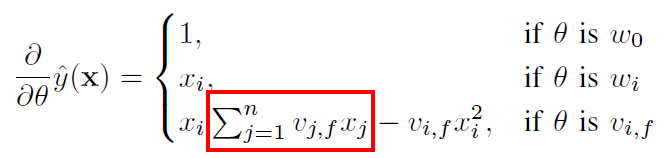
\includegraphics{FINAL/images/FM_partials_Rendle2010.png}
\caption{FM factor}
\end{figure}

    \begin{Verbatim}[commandchars=\\\{\}]
{\color{incolor}In [{\color{incolor}2}]:} \PY{k}{def} \PY{n+nf}{estimateGradientToy}\PY{p}{(}\PY{n}{record}\PY{p}{,} \PY{n}{k}\PY{p}{,} \PY{n}{b}\PY{p}{,} \PY{n}{w}\PY{p}{,} \PY{n}{V}\PY{p}{)}\PY{p}{:}
            \PY{l+s+sd}{\PYZdq{}\PYZdq{}\PYZdq{}}
        \PY{l+s+sd}{        Compute the predicted probability AND return the gradients}
        \PY{l+s+sd}{        Args:}
        \PY{l+s+sd}{            record \PYZhy{} label followed by binarized feature values}
        \PY{l+s+sd}{        Model:}
        \PY{l+s+sd}{            b \PYZhy{} bias term (scalar)}
        \PY{l+s+sd}{            w \PYZhy{} linear weight vector (array)}
        \PY{l+s+sd}{            k \PYZhy{} number of factors (def=2)}
        \PY{l+s+sd}{            V \PYZhy{} factor matrix of size (d dimensions, k=2 factors)}
        \PY{l+s+sd}{        Returns:}
        \PY{l+s+sd}{            pair \PYZhy{} ([label, predicted probability], [set of weight vectors in csr\PYZus{}matrix format])}
        \PY{l+s+sd}{    \PYZdq{}\PYZdq{}\PYZdq{}}
            
            \PY{n}{label} \PY{o}{=} \PY{n}{record}\PY{p}{[}\PY{l+m+mi}{0}\PY{p}{]}
            \PY{n}{feats} \PY{o}{=} \PY{n}{record}\PY{p}{[}\PY{l+m+mi}{1}\PY{p}{:}\PY{p}{]}
            
            \PY{c+c1}{\PYZsh{} calculate P\PYZhy{}hat    }
            \PY{c+c1}{\PYZsh{} start with linear weight dot product (X dot W)}
            \PY{n}{linear\PYZus{}sum} \PY{o}{=} \PY{n}{np}\PY{o}{.}\PY{n}{dot}\PY{p}{(}\PY{n}{w}\PY{p}{,} \PY{n}{feats}\PY{p}{)}
        
            \PY{c+c1}{\PYZsh{} factor matrix interaction sum}
            \PY{n}{factor\PYZus{}sum} \PY{o}{=} \PY{l+m+mf}{0.0}
            \PY{n}{lh\PYZus{}factor} \PY{o}{=} \PY{p}{[}\PY{l+m+mf}{0.0}\PY{p}{]}\PY{o}{*}\PY{n}{k}
            \PY{n}{rh\PYZus{}factor} \PY{o}{=} \PY{p}{[}\PY{l+m+mf}{0.0}\PY{p}{]}\PY{o}{*}\PY{n}{k}
            \PY{k}{for} \PY{n}{f} \PY{o+ow}{in} \PY{n+nb}{range}\PY{p}{(}\PY{l+m+mi}{0}\PY{p}{,} \PY{n}{k}\PY{p}{)}\PY{p}{:}
                \PY{n}{lh\PYZus{}factor}\PY{p}{[}\PY{n}{f}\PY{p}{]} \PY{o}{=} \PY{n}{np}\PY{o}{.}\PY{n}{dot}\PY{p}{(}\PY{n}{V}\PY{p}{[}\PY{n}{f}\PY{p}{]}\PY{p}{[}\PY{p}{:}\PY{p}{]}\PY{p}{,} \PY{n}{feats}\PY{p}{)}  \PY{c+c1}{\PYZsh{} we take dot product of ALL elements of the feature vector}
                \PY{n}{rh\PYZus{}factor}\PY{p}{[}\PY{n}{f}\PY{p}{]} \PY{o}{=} \PY{n}{np}\PY{o}{.}\PY{n}{dot}\PY{p}{(}\PY{n}{V}\PY{p}{[}\PY{n}{f}\PY{p}{]}\PY{p}{[}\PY{p}{:}\PY{p}{]}\PY{o}{*}\PY{o}{*}\PY{l+m+mi}{2}\PY{p}{,} \PY{n}{feats}\PY{o}{*}\PY{o}{*}\PY{l+m+mi}{2}\PY{p}{)}
                \PY{n}{factor\PYZus{}sum} \PY{o}{+}\PY{o}{=} \PY{p}{(}\PY{n}{lh\PYZus{}factor}\PY{p}{[}\PY{n}{f}\PY{p}{]}\PY{o}{*}\PY{o}{*}\PY{l+m+mi}{2} \PY{o}{\PYZhy{}} \PY{n}{rh\PYZus{}factor}\PY{p}{[}\PY{n}{f}\PY{p}{]}\PY{p}{)}
            \PY{n}{factor\PYZus{}sum} \PY{o}{=} \PY{l+m+mf}{0.5} \PY{o}{*} \PY{n}{factor\PYZus{}sum}
            
            \PY{n}{y\PYZus{}hat} \PY{o}{=} \PY{n}{b} \PY{o}{+} \PY{n}{linear\PYZus{}sum} \PY{o}{+} \PY{n}{factor\PYZus{}sum}
            
            \PY{n}{p\PYZus{}hat} \PY{o}{=} \PY{l+m+mf}{1.0} \PY{o}{/} \PY{p}{(}\PY{l+m+mi}{1} \PY{o}{+} \PY{n+nb}{float}\PY{p}{(}\PY{n}{np}\PY{o}{.}\PY{n}{exp}\PY{p}{(}\PY{o}{\PYZhy{}}\PY{n}{y\PYZus{}hat}\PY{p}{)}\PY{p}{)}\PY{p}{)}  \PY{c+c1}{\PYZsh{}logit transformation}
            
            \PY{c+c1}{\PYZsh{}compute Gradients}
            \PY{n}{b\PYZus{}grad} \PY{o}{=} \PY{n}{p\PYZus{}hat} \PY{o}{\PYZhy{}} \PY{n}{label}    \PY{c+c1}{\PYZsh{}the partial derivative of log\PYZhy{}loss function wrt constant beta}
            
            \PY{n}{w\PYZus{}grad} \PY{o}{=} \PY{n}{b\PYZus{}grad}\PY{o}{*}\PY{n}{feats}
            
            \PY{n}{v\PYZus{}data} \PY{o}{=} \PY{n}{np}\PY{o}{.}\PY{n}{array}\PY{p}{(}\PY{p}{[}\PY{p}{]}\PY{p}{)}
            \PY{k}{for} \PY{n}{f} \PY{o+ow}{in} \PY{n+nb}{range}\PY{p}{(}\PY{l+m+mi}{0}\PY{p}{,} \PY{n}{k}\PY{p}{)}\PY{p}{:}
                \PY{c+c1}{\PYZsh{} this would be too many (unnecessary) computations on a very large, sparse feature set}
                \PY{n}{v\PYZus{}data} \PY{o}{=} \PY{n}{np}\PY{o}{.}\PY{n}{append}\PY{p}{(}\PY{n}{v\PYZus{}data}\PY{p}{,} \PY{n}{b\PYZus{}grad}\PY{o}{*}\PY{p}{(}\PY{n}{lh\PYZus{}factor}\PY{p}{[}\PY{n}{f}\PY{p}{]}\PY{o}{*}\PY{n}{feats} \PY{o}{\PYZhy{}} \PY{n}{np}\PY{o}{.}\PY{n}{multiply}\PY{p}{(}\PY{n}{V}\PY{p}{[}\PY{n}{f}\PY{p}{]}\PY{p}{[}\PY{p}{:}\PY{p}{]}\PY{p}{,} \PY{n}{feats}\PY{o}{*}\PY{o}{*}\PY{l+m+mi}{2}\PY{p}{)}\PY{p}{)}\PY{p}{)}
            \PY{n}{v\PYZus{}grad} \PY{o}{=} \PY{n}{np}\PY{o}{.}\PY{n}{reshape}\PY{p}{(}\PY{n}{v\PYZus{}data}\PY{p}{,} \PY{n}{newshape}\PY{o}{=}\PY{p}{(}\PY{n}{k}\PY{p}{,} \PY{n}{V}\PY{o}{.}\PY{n}{shape}\PY{p}{[}\PY{l+m+mi}{1}\PY{p}{]}\PY{p}{)}\PY{p}{)}
            
            \PY{k}{return} \PY{p}{(}\PY{p}{[}\PY{n}{label}\PY{p}{,} \PY{n}{p\PYZus{}hat}\PY{p}{]}\PY{p}{,} \PY{p}{[}\PY{n}{b\PYZus{}grad}\PY{p}{,} \PY{n}{w\PYZus{}grad}\PY{p}{,} \PY{n}{v\PYZus{}grad}\PY{p}{]}\PY{p}{)}
\end{Verbatim}

    \begin{Verbatim}[commandchars=\\\{\}]
{\color{incolor}In [{\color{incolor}26}]:} \PY{c+c1}{\PYZsh{} for one example}
         \PY{n}{gradient} \PY{o}{=} \PY{n}{estimateGradientToy}\PY{p}{(}\PY{n}{oneHotData}\PY{p}{[}\PY{l+m+mi}{0}\PY{p}{]}\PY{p}{,} \PY{n}{k}\PY{p}{,} \PY{n}{b}\PY{p}{,} \PY{n}{w\PYZus{}vector}\PY{p}{,} \PY{n}{V\PYZus{}matrix}\PY{p}{)}
         \PY{n+nb}{print}\PY{p}{(}\PY{l+s+s2}{\PYZdq{}}\PY{l+s+s2}{(Label, predicted probability), [beta, w vector, V matrix]:}\PY{l+s+s2}{\PYZdq{}}\PY{p}{)}
         \PY{n}{gradient}
\end{Verbatim}

    \begin{Verbatim}[commandchars=\\\{\}]
(Label, predicted probability), [beta, w vector, V matrix]:

    \end{Verbatim}

\begin{Verbatim}[commandchars=\\\{\}]
{\color{outcolor}Out[{\color{outcolor}26}]:} ([1.0, 0.5024168636288922],
          [-0.49758313637110785,
           array([-0.49758314, -0.        , -0.49758314, -0.        , -0.49758314,
                  -0.49758314, -0.        , -0.49758314, -0.        , -0.        ,
                  -0.49758314, -0.        , -0.        , -0.        , -0.        ,
                  -0.        , -0.49758314, -0.        , -0.        , -0.49758314,
                  -0.        , -0.        , -0.        , -0.49758314]),
           array([[-0.051016  , -0.        , -0.03645439, -0.        , -0.03854385,
                   -0.02986771, -0.        , -0.03737504, -0.        , -0.        ,
                   -0.02509388, -0.        , -0.        , -0.        , -0.        ,
                   -0.        , -0.05390807, -0.        , -0.        , -0.01865564,
                   -0.        , -0.        , -0.        , -0.04345672],
                  [ 0.0244058 , -0.        ,  0.02071585, -0.        ,  0.02966948,
                    0.03270131,  0.        ,  0.01629193,  0.        , -0.        ,
                    0.03281537, -0.        , -0.        , -0.        , -0.        ,
                   -0.        ,  0.02478096,  0.        ,  0.        ,  0.02006145,
                    0.        ,  0.        ,  0.        ,  0.03295628]])])
\end{Verbatim}
            
    We calculate the log-loss based on our current set of predictions and
their actual click outcomes. This will be useful later when we
iteratively update the model until we see a decline in further
improvement.

    \[logloss = -\frac{1}{N}\sum_{i=1}^{N}[y_i\cdot log p_i + (1-p_i)\cdot log(1-p_i)]\]

    \begin{Verbatim}[commandchars=\\\{\}]
{\color{incolor}In [{\color{incolor}10}]:} \PY{k}{def} \PY{n+nf}{logLossToy}\PY{p}{(}\PY{n}{pair}\PY{p}{)}\PY{p}{:}
             \PY{l+s+sd}{\PYZdq{}\PYZdq{}\PYZdq{}parallelize log loss}
         \PY{l+s+sd}{        input: ([label, prob], [b\PYZus{}grad, w\PYZus{}grad, v\PYZus{}grad])}
         \PY{l+s+sd}{    \PYZdq{}\PYZdq{}\PYZdq{}}
             \PY{n}{y} \PY{o}{=} \PY{n}{pair}\PY{p}{[}\PY{l+m+mi}{0}\PY{p}{]}\PY{p}{[}\PY{l+m+mi}{1}\PY{p}{]}
             
             \PY{n}{eps} \PY{o}{=} \PY{l+m+mf}{1.0e\PYZhy{}16}
             \PY{k}{if} \PY{n}{pair}\PY{p}{[}\PY{l+m+mi}{0}\PY{p}{]}\PY{p}{[}\PY{l+m+mi}{1}\PY{p}{]} \PY{o}{==} \PY{l+m+mi}{0}\PY{p}{:}
                 \PY{n}{p\PYZus{}hat} \PY{o}{=} \PY{n}{eps}
             \PY{k}{elif} \PY{n}{pair}\PY{p}{[}\PY{l+m+mi}{0}\PY{p}{]}\PY{p}{[}\PY{l+m+mi}{1}\PY{p}{]} \PY{o}{==} \PY{l+m+mi}{1}\PY{p}{:}
                 \PY{n}{p\PYZus{}hat} \PY{o}{=} \PY{l+m+mi}{1}\PY{o}{\PYZhy{}}\PY{n}{eps}
             \PY{k}{else}\PY{p}{:}
                 \PY{n}{p\PYZus{}hat} \PY{o}{=} \PY{n}{pair}\PY{p}{[}\PY{l+m+mi}{0}\PY{p}{]}\PY{p}{[}\PY{l+m+mi}{1}\PY{p}{]}
             
             \PY{k}{return} \PY{n+nb}{float}\PY{p}{(}\PY{o}{\PYZhy{}}\PY{p}{(}\PY{n}{y} \PY{o}{*} \PY{n}{np}\PY{o}{.}\PY{n}{log}\PY{p}{(}\PY{n}{p\PYZus{}hat}\PY{p}{)} \PY{o}{+} \PY{p}{(}\PY{l+m+mi}{1}\PY{o}{\PYZhy{}}\PY{n}{y}\PY{p}{)} \PY{o}{*} \PY{n}{np}\PY{o}{.}\PY{n}{log}\PY{p}{(}\PY{l+m+mi}{1}\PY{o}{\PYZhy{}}\PY{n}{p\PYZus{}hat}\PY{p}{)}\PY{p}{)}\PY{p}{)}
\end{Verbatim}

    \begin{Verbatim}[commandchars=\\\{\}]
{\color{incolor}In [{\color{incolor}11}]:} \PY{n}{logLossToy}\PY{p}{(}\PY{n}{gradient}\PY{p}{)}
\end{Verbatim}

\begin{Verbatim}[commandchars=\\\{\}]
{\color{outcolor}Out[{\color{outcolor}11}]:} 0.6931354980548503
\end{Verbatim}
            
    We then use the partial gradients calculated in
\texttt{estimateGradientToy} and combine those using a reduce and then
update our weight vectors by subtracting off the gradient times a
learning rate. This would then feed back into a new set of model
predictions, a new calculation of loss, and then continued updates of
the model, either until the loss converges or a set number of
iterations.

    \begin{Verbatim}[commandchars=\\\{\}]
{\color{incolor}In [{\color{incolor}24}]:} \PY{c+c1}{\PYZsh{} update weights}
         \PY{n}{learningRate} \PY{o}{=} \PY{l+m+mf}{0.1}
         
         \PY{c+c1}{\PYZsh{} initialize gradient}
         \PY{n}{wGrad\PYZus{}reduce} \PY{o}{=} \PY{n}{np}\PY{o}{.}\PY{n}{zeros}\PY{p}{(}\PY{p}{(}\PY{l+m+mi}{1}\PY{p}{,} \PY{n}{numFeats}\PY{p}{)}\PY{p}{)}
         
         \PY{c+c1}{\PYZsh{} aggregate partial gradients while iterating over rows}
         \PY{k}{for} \PY{n}{r} \PY{o+ow}{in} \PY{n+nb}{range}\PY{p}{(}\PY{l+m+mi}{0}\PY{p}{,} \PY{n}{nrow}\PY{p}{)}\PY{p}{:}
             \PY{n}{gradient} \PY{o}{=} \PY{n}{estimateGradientToy}\PY{p}{(}\PY{n}{oneHotData}\PY{p}{[}\PY{n}{r}\PY{p}{]}\PY{p}{,} \PY{n}{k}\PY{p}{,} \PY{n}{b}\PY{p}{,} \PY{n}{w\PYZus{}vector}\PY{p}{,} \PY{n}{V\PYZus{}matrix}\PY{p}{)}
             \PY{n}{wGrad\PYZus{}reduce} \PY{o}{+}\PY{o}{=} \PY{n}{gradient}\PY{p}{[}\PY{l+m+mi}{1}\PY{p}{]}\PY{p}{[}\PY{l+m+mi}{1}\PY{p}{]}
             
         \PY{c+c1}{\PYZsh{} calculate average gradient}
         \PY{n}{w\PYZus{}update} \PY{o}{=} \PY{n}{wGrad\PYZus{}reduce} \PY{o}{/} \PY{n}{nrow}
         
         \PY{c+c1}{\PYZsh{} update weight vector}
         \PY{n}{w\PYZus{}new} \PY{o}{=} \PY{n}{w\PYZus{}vector} \PY{o}{\PYZhy{}} \PY{n}{learningRate}\PY{o}{*}\PY{n}{w\PYZus{}update}
         
         \PY{n+nb}{print}\PY{p}{(}\PY{l+s+s2}{\PYZdq{}}\PY{l+s+s2}{New weight vector W}\PY{l+s+s2}{\PYZdq{}}\PY{p}{)}
         \PY{n}{w\PYZus{}new}\PY{o}{.}\PY{n}{T}
\end{Verbatim}

    \begin{Verbatim}[commandchars=\\\{\}]
New weight vector W

    \end{Verbatim}

\begin{Verbatim}[commandchars=\\\{\}]
{\color{outcolor}Out[{\color{outcolor}24}]:} array([[-0.03310685],
                [ 0.01428775],
                [-0.00376144],
                [-0.015721  ],
                [ 0.02960499],
                [ 0.02180846],
                [-0.001696  ],
                [ 0.01552031],
                [-0.01699597],
                [-0.01138352],
                [ 0.02639799],
                [-0.01805496],
                [-0.00738271],
                [-0.01722051],
                [-0.02619963],
                [-0.03151945],
                [ 0.04281266],
                [-0.04104915],
                [-0.02042689],
                [ 0.01739337],
                [ 0.01881405],
                [-0.04028339],
                [-0.02320497],
                [ 0.00714665]])
\end{Verbatim}
            
    \begin{Verbatim}[commandchars=\\\{\}]
{\color{incolor}In [{\color{incolor}23}]:} \PY{c+c1}{\PYZsh{} repeat process to update V matrix}
         
         \PY{n}{vGrad\PYZus{}reduce} \PY{o}{=} \PY{n}{np}\PY{o}{.}\PY{n}{zeros}\PY{p}{(}\PY{p}{(}\PY{n}{k}\PY{p}{,} \PY{n}{numFeats}\PY{p}{)}\PY{p}{)}
         \PY{k}{for} \PY{n}{r} \PY{o+ow}{in} \PY{n+nb}{range}\PY{p}{(}\PY{l+m+mi}{0}\PY{p}{,} \PY{n}{nrow}\PY{p}{)}\PY{p}{:}
             \PY{n}{gradient} \PY{o}{=} \PY{n}{estimateGradientToy}\PY{p}{(}\PY{n}{oneHotData}\PY{p}{[}\PY{n}{r}\PY{p}{]}\PY{p}{,} \PY{n}{k}\PY{p}{,} \PY{n}{b}\PY{p}{,} \PY{n}{w\PYZus{}vector}\PY{p}{,} \PY{n}{V\PYZus{}matrix}\PY{p}{)}
             \PY{n}{vGrad\PYZus{}reduce} \PY{o}{+}\PY{o}{=} \PY{n}{gradient}\PY{p}{[}\PY{l+m+mi}{1}\PY{p}{]}\PY{p}{[}\PY{l+m+mi}{2}\PY{p}{]}
         \PY{n}{v\PYZus{}update} \PY{o}{=} \PY{n}{vGrad\PYZus{}reduce} \PY{o}{/} \PY{n}{nrow}
         
         \PY{n}{V\PYZus{}new} \PY{o}{=} \PY{n}{V\PYZus{}matrix} \PY{o}{\PYZhy{}} \PY{n}{learningRate}\PY{o}{*}\PY{n}{v\PYZus{}update}
         
         \PY{n+nb}{print}\PY{p}{(}\PY{l+s+s2}{\PYZdq{}}\PY{l+s+s2}{New factor matrix V weights:}\PY{l+s+s2}{\PYZdq{}}\PY{p}{)}
         \PY{n}{V\PYZus{}new}\PY{o}{.}\PY{n}{T}
\end{Verbatim}

    \begin{Verbatim}[commandchars=\\\{\}]
New factor matrix V weights:

    \end{Verbatim}

\begin{Verbatim}[commandchars=\\\{\}]
{\color{outcolor}Out[{\color{outcolor}23}]:} array([[-0.01659269, -0.0107129 ],
                [-0.00526753, -0.01770845],
                [ 0.01061032, -0.01639128],
                [ 0.03818184, -0.00625369],
                [ 0.00782152, -0.00024604],
                [ 0.02496888,  0.00574602],
                [ 0.01363172,  0.01560516],
                [ 0.01013153, -0.02668518],
                [ 0.01761522,  0.00018196],
                [-0.06089243, -0.03704973],
                [ 0.03440378,  0.00597145],
                [ 0.01331686, -0.01696164],
                [ 0.02983592, -0.01582817],
                [ 0.02259963, -0.04301197],
                [ 0.00912995, -0.01519263],
                [-0.00842256, -0.00671412],
                [-0.02254404, -0.00990762],
                [-0.01389515,  0.01140745],
                [-0.00252248,  0.00297071],
                [ 0.04712819, -0.01923517],
                [-0.01277656,  0.01345092],
                [ 0.0081833 ,  0.02907576],
                [ 0.02244913,  0.00251953],
                [-0.00188818,  0.00624993]])
\end{Verbatim}
            
    \section{3. Exploration of Criteo Training
Dataset}\label{exploration-of-criteo-training-dataset}

We begin by exploring a sample of our training dataset's numeric and
categorical features, understanding their distributions and potential
sparsity, and consider how we can best transform them into features
efficiently used by FM.

    \begin{Verbatim}[commandchars=\\\{\}]
{\color{incolor}In [{\color{incolor}5}]:} \PY{c+c1}{\PYZsh{} imports}
        \PY{k+kn}{import} \PY{n+nn}{numpy} \PY{k}{as} \PY{n+nn}{np}
        \PY{k+kn}{import} \PY{n+nn}{pandas} \PY{k}{as} \PY{n+nn}{pd}
        
        \PY{c+c1}{\PYZsh{} visuals}
        \PY{k+kn}{import} \PY{n+nn}{seaborn} \PY{k}{as} \PY{n+nn}{sns}
        \PY{k+kn}{import} \PY{n+nn}{matplotlib}\PY{n+nn}{.}\PY{n+nn}{pyplot} \PY{k}{as} \PY{n+nn}{plt}
        \PY{k+kn}{from} \PY{n+nn}{matplotlib}\PY{n+nn}{.}\PY{n+nn}{pyplot} \PY{k}{import} \PY{n}{figure}
        
        \PY{k+kn}{import} \PY{n+nn}{time}
        \PY{k+kn}{from} \PY{n+nn}{scipy}\PY{n+nn}{.}\PY{n+nn}{sparse} \PY{k}{import} \PY{n}{csr\PYZus{}matrix}
        \PY{k+kn}{from} \PY{n+nn}{pyspark}\PY{n+nn}{.}\PY{n+nn}{sql} \PY{k}{import} \PY{n}{Row}
        \PY{k+kn}{from} \PY{n+nn}{pyspark}\PY{n+nn}{.}\PY{n+nn}{ml}\PY{n+nn}{.}\PY{n+nn}{feature} \PY{k}{import} \PY{n}{CountVectorizer}
        \PY{k+kn}{from} \PY{n+nn}{pyspark}\PY{n+nn}{.}\PY{n+nn}{sql} \PY{k}{import} \PY{n}{DataFrame}
\end{Verbatim}

    \begin{Verbatim}[commandchars=\\\{\}]
{\color{incolor}In [{\color{incolor}6}]:} \PY{c+c1}{\PYZsh{} start Spark Session}
        \PY{k+kn}{from} \PY{n+nn}{pyspark}\PY{n+nn}{.}\PY{n+nn}{sql} \PY{k}{import} \PY{n}{SparkSession}
        \PY{n}{app\PYZus{}name} \PY{o}{=} \PY{l+s+s2}{\PYZdq{}}\PY{l+s+s2}{w261FinalProject}\PY{l+s+s2}{\PYZdq{}}
        \PY{n}{master} \PY{o}{=} \PY{l+s+s2}{\PYZdq{}}\PY{l+s+s2}{local[*]}\PY{l+s+s2}{\PYZdq{}}
        \PY{n}{spark} \PY{o}{=} \PY{n}{SparkSession}\PYZbs{}
                \PY{o}{.}\PY{n}{builder}\PYZbs{}
                \PY{o}{.}\PY{n}{appName}\PY{p}{(}\PY{n}{app\PYZus{}name}\PY{p}{)}\PYZbs{}
                \PY{o}{.}\PY{n}{master}\PY{p}{(}\PY{n}{master}\PY{p}{)}\PYZbs{}
                \PY{o}{.}\PY{n}{getOrCreate}\PY{p}{(}\PY{p}{)}
        \PY{n}{sc} \PY{o}{=} \PY{n}{spark}\PY{o}{.}\PY{n}{sparkContext}
\end{Verbatim}

    Our team performed our EDA using a sample of \textasciitilde{}230,000
observations from the training data. The EDA results are first presented
on the numerical data in the Criteo display advertising dataset in order
to understand the distributions of their values, their correlations, and
the extent of missing data. We then present the EDA results for the
categorical data in order to also understand their frequency
distributions and missing values. Most of these analyses were performed
with a sub-sample of 5000 observations. These details and results
informed our transformations and representation of the data.

    \subsubsection{Load Training Data Sample for Local
Testing}\label{load-training-data-sample-for-local-testing}

    \begin{Verbatim}[commandchars=\\\{\}]
{\color{incolor}In [{\color{incolor}7}]:} \PY{n}{original\PYZus{}trainRDD} \PY{o}{=} \PY{n}{sc}\PY{o}{.}\PY{n}{textFile}\PY{p}{(}\PY{l+s+s1}{\PYZsq{}}\PY{l+s+s1}{data/train.txt}\PY{l+s+s1}{\PYZsq{}}\PY{p}{)}
        
        \PY{n}{splits} \PY{o}{=} \PY{l+m+mf}{0.005}
        
        \PY{n}{largeRDD}\PY{p}{,} \PY{n}{smallTestRDD}\PY{p}{,} \PY{n}{smallTrainRDD} \PY{o}{=} \PY{n}{original\PYZus{}trainRDD}\PY{o}{.}\PY{n}{randomSplit}\PY{p}{(}\PY{p}{[}\PY{l+m+mi}{1}\PY{o}{\PYZhy{}}\PY{l+m+mi}{2}\PY{o}{*}\PY{n}{splits}\PY{p}{,} \PY{n}{splits}\PY{p}{,} \PY{n}{splits}\PY{p}{]}\PY{p}{,} \PY{n}{seed} \PY{o}{=} \PY{l+m+mi}{1}\PY{p}{)}
        \PY{n}{smallTrainRDD}\PY{o}{.}\PY{n}{cache}\PY{p}{(}\PY{p}{)}
        
        \PY{n}{ncol} \PY{o}{=} \PY{n+nb}{len}\PY{p}{(}\PY{n}{smallTrainRDD}\PY{o}{.}\PY{n}{take}\PY{p}{(}\PY{l+m+mi}{1}\PY{p}{)}\PY{p}{[}\PY{l+m+mi}{0}\PY{p}{]}\PY{o}{.}\PY{n}{split}\PY{p}{(}\PY{l+s+s1}{\PYZsq{}}\PY{l+s+se}{\PYZbs{}t}\PY{l+s+s1}{\PYZsq{}}\PY{p}{)}\PY{p}{)}
        \PY{n}{nrow} \PY{o}{=} \PY{n}{smallTrainRDD}\PY{o}{.}\PY{n}{count}\PY{p}{(}\PY{p}{)}
        \PY{n+nb}{print}\PY{p}{(}\PY{n}{f}\PY{l+s+s1}{\PYZsq{}}\PY{l+s+s1}{This sample contains }\PY{l+s+si}{\PYZob{}nrow\PYZcb{}}\PY{l+s+s1}{ rows and }\PY{l+s+si}{\PYZob{}ncol\PYZcb{}}\PY{l+s+s1}{ columns}\PY{l+s+s1}{\PYZsq{}}\PY{p}{)}
\end{Verbatim}

    \begin{Verbatim}[commandchars=\\\{\}]
This sample contains 229937 rows and 40 columns

    \end{Verbatim}

    \subsubsection{\texorpdfstring{\emph{Numeric
Variables}}{Numeric Variables}}\label{numeric-variables}

    Below, the numerical features are extracted for EDA.

    \begin{Verbatim}[commandchars=\\\{\}]
{\color{incolor}In [{\color{incolor}5}]:} \PY{k}{def} \PY{n+nf}{parse\PYZus{}numbers}\PY{p}{(}\PY{n}{line}\PY{p}{)}\PY{p}{:}
            \PY{l+s+sd}{\PYZdq{}\PYZdq{}\PYZdq{}}
        \PY{l+s+sd}{    This function selects the numerical variables from the dataset for EDA}
        \PY{l+s+sd}{    \PYZdq{}\PYZdq{}\PYZdq{}}
            \PY{n}{fields} \PY{o}{=} \PY{n}{np}\PY{o}{.}\PY{n}{array}\PY{p}{(}\PY{n}{line}\PY{o}{.}\PY{n}{split}\PY{p}{(}\PY{l+s+s1}{\PYZsq{}}\PY{l+s+se}{\PYZbs{}t}\PY{l+s+s1}{\PYZsq{}}\PY{p}{)}\PY{p}{[}\PY{p}{:}\PY{l+m+mi}{14}\PY{p}{]}\PY{p}{)}
            \PY{n}{label}\PY{p}{,}\PY{n}{features} \PY{o}{=} \PY{n}{fields}\PY{p}{[}\PY{l+m+mi}{0}\PY{p}{]}\PY{p}{,} \PY{n}{fields}\PY{p}{[}\PY{l+m+mi}{1}\PY{p}{:}\PY{p}{]}
            \PY{k}{return}\PY{p}{(}\PY{n}{features}\PY{p}{,} \PY{n}{label}\PY{p}{)}
\end{Verbatim}

    \begin{Verbatim}[commandchars=\\\{\}]
{\color{incolor}In [{\color{incolor}6}]:} \PY{n}{numeric\PYZus{}trainRDDCached} \PY{o}{=} \PY{n}{smallTrainRDD}\PY{o}{.}\PY{n}{map}\PY{p}{(}\PY{n}{parse\PYZus{}numbers}\PY{p}{)}\PY{o}{.}\PY{n}{cache}\PY{p}{(}\PY{p}{)}
        \PY{n}{numeric\PYZus{}sample} \PY{o}{=} \PY{n}{np}\PY{o}{.}\PY{n}{array}\PY{p}{(}\PY{n}{numeric\PYZus{}trainRDDCached}\PY{o}{.}\PY{n}{map}\PY{p}{(}\PY{k}{lambda} \PY{n}{x}\PY{p}{:} \PY{n}{np}\PY{o}{.}\PY{n}{append}\PY{p}{(}\PY{n}{x}\PY{p}{[}\PY{l+m+mi}{0}\PY{p}{]}\PY{p}{,} \PY{p}{[}\PY{n}{x}\PY{p}{[}\PY{l+m+mi}{1}\PY{p}{]}\PY{p}{]}\PY{p}{)}\PY{p}{)}\PY{o}{.}\PY{n}{takeSample}\PY{p}{(}\PY{k+kc}{False}\PY{p}{,} \PY{l+m+mi}{5000}\PY{p}{)}\PY{p}{)}\PY{c+c1}{\PYZsh{}sub\PYZhy{}sample}
        \PY{n}{numeric\PYZus{}sample\PYZus{}df} \PY{o}{=} \PY{n}{pd}\PY{o}{.}\PY{n}{DataFrame}\PY{p}{(}\PY{n}{np}\PY{o}{.}\PY{n}{array}\PY{p}{(}\PY{n}{numeric\PYZus{}sample}\PY{p}{)}\PY{p}{)}
\end{Verbatim}

    The first 5 rows of the EDA sample (numerical only) are shown below to
give an example of the numerical features.

    \begin{Verbatim}[commandchars=\\\{\}]
{\color{incolor}In [{\color{incolor}8}]:} \PY{n+nb}{print}\PY{p}{(}\PY{l+s+s2}{\PYZdq{}}\PY{l+s+s2}{Example of Numerical Features Extracted:}\PY{l+s+s2}{\PYZdq{}}\PY{p}{)}
        \PY{n}{numeric\PYZus{}sample\PYZus{}df}\PY{o}{.}\PY{n}{head}\PY{p}{(}\PY{p}{)}
\end{Verbatim}

    \begin{Verbatim}[commandchars=\\\{\}]
Example of Numerical Features Extracted:

    \end{Verbatim}

\begin{Verbatim}[commandchars=\\\{\}]
{\color{outcolor}Out[{\color{outcolor}8}]:}   0   1   2   3      4   5   6   7    8  9   10 11  12 13
        0  0  -1   5   2     12  61   4  45  102  0   2      2  0
        1  6  19   6   9     24  10  25   9    9  2  11  1   9  0
        2  1  24   2   1    210  11   8  12  260  1   6      1  1
        3      7  35  17  11232       0  17   45      0     17  0
        4     84  25  11    217       0  15   14      0  1  14  1
\end{Verbatim}
            
    \begin{Verbatim}[commandchars=\\\{\}]
{\color{incolor}In [{\color{incolor}16}]:} \PY{n}{numeric\PYZus{}sample\PYZus{}df} \PY{o}{=} \PY{n}{numeric\PYZus{}sample\PYZus{}df}\PY{o}{.}\PY{n}{apply}\PY{p}{(}\PY{n}{pd}\PY{o}{.}\PY{n}{to\PYZus{}numeric}\PY{p}{)}
\end{Verbatim}

    The histograms of each numerical feature are shown below. The 13th
column holds the outcome variable.

    \begin{Verbatim}[commandchars=\\\{\}]
{\color{incolor}In [{\color{incolor}17}]:} \PY{n}{numeric\PYZus{}sample\PYZus{}df}\PY{o}{.}\PY{n}{hist}\PY{p}{(}\PY{n}{figsize}\PY{o}{=}\PY{p}{(}\PY{l+m+mi}{25}\PY{p}{,}\PY{l+m+mi}{25}\PY{p}{)}\PY{p}{,} \PY{n}{bins}\PY{o}{=}\PY{l+m+mi}{100}\PY{p}{)}
         \PY{n}{plt}\PY{o}{.}\PY{n}{show}\PY{p}{(}\PY{p}{)}
\end{Verbatim}

    \begin{center}
    \adjustimage{max size={0.9\linewidth}{0.9\paperheight}}{output_49_0.png}
    \end{center}
    { \hspace*{\fill} \\}
    
    All of the independent numerical variables, with the exception of the
10th numerical variable (index 9), show a very strong right (positive)
skew, which suggests that a log-transform might be helpful. The above
distributions also provide guidance on bucketing criteria in the
subsequent data transformation. Next, we use a series of boxplots to
identify any obvious correlations between the independent numerical
variables and the click through response.

    \begin{Verbatim}[commandchars=\\\{\}]
{\color{incolor}In [{\color{incolor}28}]:} \PY{n}{fig}\PY{p}{,} \PY{n}{ax\PYZus{}grid} \PY{o}{=} \PY{n}{plt}\PY{o}{.}\PY{n}{subplots}\PY{p}{(}\PY{l+m+mi}{5}\PY{p}{,} \PY{l+m+mi}{3}\PY{p}{,} \PY{n}{figsize}\PY{o}{=}\PY{p}{(}\PY{l+m+mi}{15}\PY{p}{,}\PY{l+m+mi}{15}\PY{p}{)}\PY{p}{)}
         \PY{n}{y} \PY{o}{=} \PY{n}{numeric\PYZus{}sample\PYZus{}df}\PY{o}{.}\PY{n}{loc}\PY{p}{[}\PY{p}{:}\PY{p}{,}\PY{l+m+mi}{13}\PY{p}{]}\PY{c+c1}{\PYZsh{}.astype(\PYZdq{}float\PYZdq{})}
         \PY{k}{for} \PY{n}{idx} \PY{o+ow}{in} \PY{n+nb}{range}\PY{p}{(}\PY{n+nb}{len}\PY{p}{(}\PY{n}{numeric\PYZus{}sample\PYZus{}df}\PY{o}{.}\PY{n}{columns}\PY{p}{)}\PY{o}{\PYZhy{}}\PY{l+m+mi}{1}\PY{p}{)}\PY{p}{:}
             \PY{n}{x} \PY{o}{=} \PY{n}{numeric\PYZus{}sample\PYZus{}df}\PY{o}{.}\PY{n}{loc}\PY{p}{[}\PY{p}{:}\PY{p}{,}\PY{n}{idx}\PY{p}{]}
             \PY{n}{sns}\PY{o}{.}\PY{n}{boxplot}\PY{p}{(}\PY{n}{x}\PY{p}{,} \PY{n}{y}\PY{p}{,} \PY{n}{ax}\PY{o}{=}\PY{n}{ax\PYZus{}grid}\PY{p}{[}\PY{n}{idx}\PY{o}{/}\PY{o}{/}\PY{l+m+mi}{3}\PY{p}{]}\PY{p}{[}\PY{n}{idx}\PY{o}{\PYZpc{}}\PY{k}{3}], orient=\PYZsq{}h\PYZsq{}, linewidth=.5)
             \PY{n}{ax\PYZus{}grid}\PY{p}{[}\PY{n}{idx}\PY{o}{/}\PY{o}{/}\PY{l+m+mi}{3}\PY{p}{]}\PY{p}{[}\PY{n}{idx}\PY{o}{\PYZpc{}}\PY{k}{3}].invert\PYZus{}yaxis()
         \PY{n}{fig}\PY{o}{.}\PY{n}{suptitle}\PY{p}{(}\PY{l+s+s2}{\PYZdq{}}\PY{l+s+s2}{Numerical Features vs. Outcome (click)}\PY{l+s+s2}{\PYZdq{}}\PY{p}{,} \PY{n}{fontsize}\PY{o}{=}\PY{l+m+mi}{15}\PY{p}{,} \PY{n}{y}\PY{o}{=}\PY{l+m+mf}{0.9}\PY{p}{)}
         \PY{n}{plt}\PY{o}{.}\PY{n}{show}\PY{p}{(}\PY{p}{)}
\end{Verbatim}

    \begin{center}
    \adjustimage{max size={0.9\linewidth}{0.9\paperheight}}{output_51_0.png}
    \end{center}
    { \hspace*{\fill} \\}
    
    There is some minor evidence that the 11th numerical feature (index 10)
has a positive correlation with click response, but the above boxplots
otherwise show no obvious correlations with the target variable. Below,
we show a heatmap of pair-wise correlations between the independent
variables to identify any strong collinearity within the dataset.

    \begin{Verbatim}[commandchars=\\\{\}]
{\color{incolor}In [{\color{incolor}29}]:} \PY{n}{corr} \PY{o}{=} \PY{n}{numeric\PYZus{}sample\PYZus{}df}\PY{o}{.}\PY{n}{loc}\PY{p}{[}\PY{p}{:}\PY{p}{,}\PY{p}{:}\PY{l+m+mi}{14}\PY{p}{]}\PY{o}{.}\PY{n}{corr}\PY{p}{(}\PY{p}{)}
         \PY{n}{fig}\PY{p}{,} \PY{n}{ax} \PY{o}{=} \PY{n}{plt}\PY{o}{.}\PY{n}{subplots}\PY{p}{(}\PY{n}{figsize}\PY{o}{=}\PY{p}{(}\PY{l+m+mi}{11}\PY{p}{,} \PY{l+m+mi}{9}\PY{p}{)}\PY{p}{)}
         \PY{n}{mask} \PY{o}{=} \PY{n}{np}\PY{o}{.}\PY{n}{zeros\PYZus{}like}\PY{p}{(}\PY{n}{corr}\PY{p}{,} \PY{n}{dtype}\PY{o}{=}\PY{n}{np}\PY{o}{.}\PY{n}{bool}\PY{p}{)}
         \PY{n}{mask}\PY{p}{[}\PY{n}{np}\PY{o}{.}\PY{n}{triu\PYZus{}indices\PYZus{}from}\PY{p}{(}\PY{n}{mask}\PY{p}{)}\PY{p}{]} \PY{o}{=} \PY{k+kc}{True}
         \PY{n}{cmap} \PY{o}{=} \PY{n}{sns}\PY{o}{.}\PY{n}{diverging\PYZus{}palette}\PY{p}{(}\PY{l+m+mi}{240}\PY{p}{,} \PY{l+m+mi}{10}\PY{p}{,} \PY{n}{as\PYZus{}cmap}\PY{o}{=}\PY{k+kc}{True}\PY{p}{)}
         \PY{n}{sns}\PY{o}{.}\PY{n}{heatmap}\PY{p}{(}\PY{n}{corr}\PY{p}{,} \PY{n}{mask}\PY{o}{=}\PY{n}{mask}\PY{p}{,} \PY{n}{cmap}\PY{o}{=}\PY{n}{cmap}\PY{p}{,} \PY{n}{center}\PY{o}{=}\PY{l+m+mi}{0}\PY{p}{,} \PY{n}{linewidths}\PY{o}{=}\PY{o}{.}\PY{l+m+mi}{5}\PY{p}{)}
         \PY{n}{plt}\PY{o}{.}\PY{n}{title}\PY{p}{(}\PY{l+s+s2}{\PYZdq{}}\PY{l+s+s2}{Correlations between features.}\PY{l+s+s2}{\PYZdq{}}\PY{p}{)}
         \PY{n}{plt}\PY{o}{.}\PY{n}{show}\PY{p}{(}\PY{p}{)}
\end{Verbatim}

    \begin{center}
    \adjustimage{max size={0.9\linewidth}{0.9\paperheight}}{output_53_0.png}
    \end{center}
    { \hspace*{\fill} \\}
    
    Numerical feature pairs 6 - 10 and 3 - 12 (by index) show evidence of a
positive correlation, but the remaining features otherwise do not
indicate strong collinearity.

    \subsubsection{\texorpdfstring{\emph{Log
Transform}}{Log Transform}}\label{log-transform}

Due to the high positive skew in the histograms of the numerical
features, we have repeated the prior EDA using the log form to assess
its potential to improve their predictive power.

    \begin{Verbatim}[commandchars=\\\{\}]
{\color{incolor}In [{\color{incolor}30}]:} \PY{n}{small\PYZus{}constant} \PY{o}{=} \PY{l+m+mf}{0.001} \PY{c+c1}{\PYZsh{}to be added since these variables contain a high number of zeros}
         \PY{n}{log\PYZus{}numeric\PYZus{}sample\PYZus{}df} \PY{o}{=} \PY{n}{numeric\PYZus{}sample\PYZus{}df}\PY{o}{.}\PY{n}{apply}\PY{p}{(}\PY{k}{lambda} \PY{n}{x}\PY{p}{:} \PY{n}{x}\PY{o}{+}\PY{n}{small\PYZus{}constant}\PY{p}{)}\PY{o}{.}\PY{n}{apply}\PY{p}{(}\PY{n}{np}\PY{o}{.}\PY{n}{log}\PY{p}{)}
\end{Verbatim}

    \begin{Verbatim}[commandchars=\\\{\}]
{\color{incolor}In [{\color{incolor}31}]:} \PY{n}{log\PYZus{}numeric\PYZus{}sample\PYZus{}df}\PY{o}{.}\PY{n}{hist}\PY{p}{(}\PY{n}{figsize}\PY{o}{=}\PY{p}{(}\PY{l+m+mi}{25}\PY{p}{,}\PY{l+m+mi}{25}\PY{p}{)}\PY{p}{,} \PY{n}{bins}\PY{o}{=}\PY{l+m+mi}{100}\PY{p}{)}
         \PY{n}{plt}\PY{o}{.}\PY{n}{show}\PY{p}{(}\PY{p}{)}
\end{Verbatim}

    \begin{center}
    \adjustimage{max size={0.9\linewidth}{0.9\paperheight}}{output_57_0.png}
    \end{center}
    { \hspace*{\fill} \\}
    
    The log transform indeed addresses the skew in the numerical features,
however, the high number of zeros in these variables results in a peak
that is distant from the distribution of non-zero raw values. Again, we
show the boxplots for each of the log-transformed variables below.

    \begin{Verbatim}[commandchars=\\\{\}]
{\color{incolor}In [{\color{incolor}32}]:} \PY{n}{fig}\PY{p}{,} \PY{n}{ax\PYZus{}grid} \PY{o}{=} \PY{n}{plt}\PY{o}{.}\PY{n}{subplots}\PY{p}{(}\PY{l+m+mi}{5}\PY{p}{,} \PY{l+m+mi}{3}\PY{p}{,} \PY{n}{figsize}\PY{o}{=}\PY{p}{(}\PY{l+m+mi}{15}\PY{p}{,}\PY{l+m+mi}{15}\PY{p}{)}\PY{p}{)}
         \PY{n}{y} \PY{o}{=} \PY{n}{numeric\PYZus{}sample\PYZus{}df}\PY{o}{.}\PY{n}{loc}\PY{p}{[}\PY{p}{:}\PY{p}{,}\PY{l+m+mi}{13}\PY{p}{]}\PY{c+c1}{\PYZsh{}.astype(\PYZdq{}float\PYZdq{})}
         \PY{k}{for} \PY{n}{idx} \PY{o+ow}{in} \PY{n+nb}{range}\PY{p}{(}\PY{n+nb}{len}\PY{p}{(}\PY{n}{numeric\PYZus{}sample\PYZus{}df}\PY{o}{.}\PY{n}{columns}\PY{p}{)}\PY{o}{\PYZhy{}}\PY{l+m+mi}{1}\PY{p}{)}\PY{p}{:}
             \PY{n}{x} \PY{o}{=} \PY{n}{log\PYZus{}numeric\PYZus{}sample\PYZus{}df}\PY{o}{.}\PY{n}{loc}\PY{p}{[}\PY{p}{:}\PY{p}{,}\PY{n}{idx}\PY{p}{]}
             \PY{n}{sns}\PY{o}{.}\PY{n}{boxplot}\PY{p}{(}\PY{n}{x}\PY{p}{,} \PY{n}{y}\PY{p}{,} \PY{n}{ax}\PY{o}{=}\PY{n}{ax\PYZus{}grid}\PY{p}{[}\PY{n}{idx}\PY{o}{/}\PY{o}{/}\PY{l+m+mi}{3}\PY{p}{]}\PY{p}{[}\PY{n}{idx}\PY{o}{\PYZpc{}}\PY{k}{3}], orient=\PYZsq{}h\PYZsq{}, linewidth=.5)
             \PY{n}{ax\PYZus{}grid}\PY{p}{[}\PY{n}{idx}\PY{o}{/}\PY{o}{/}\PY{l+m+mi}{3}\PY{p}{]}\PY{p}{[}\PY{n}{idx}\PY{o}{\PYZpc{}}\PY{k}{3}].invert\PYZus{}yaxis()
         \PY{n}{fig}\PY{o}{.}\PY{n}{suptitle}\PY{p}{(}\PY{l+s+s2}{\PYZdq{}}\PY{l+s+s2}{Numerical Features (log form) vs. Outcome (click)}\PY{l+s+s2}{\PYZdq{}}\PY{p}{,} \PY{n}{fontsize}\PY{o}{=}\PY{l+m+mi}{15}\PY{p}{,} \PY{n}{y}\PY{o}{=}\PY{l+m+mf}{0.9}\PY{p}{)}
         \PY{n}{plt}\PY{o}{.}\PY{n}{show}\PY{p}{(}\PY{p}{)}
\end{Verbatim}

    \begin{center}
    \adjustimage{max size={0.9\linewidth}{0.9\paperheight}}{output_59_0.png}
    \end{center}
    { \hspace*{\fill} \\}
    
    Similar to before, the boxplots above suggest a positive correlation
between the log form of the 11th numerical feature (index 10) and the
outcome, and additionally suggest a potential negative correlation
between the log form of the 6th numerical feature (index 5) and the
outcome. Next, we show a heatmap for pair-wise correlations of the log
transforms of the independent variables.

    \begin{Verbatim}[commandchars=\\\{\}]
{\color{incolor}In [{\color{incolor}33}]:} \PY{n}{corr} \PY{o}{=} \PY{n}{log\PYZus{}numeric\PYZus{}sample\PYZus{}df}\PY{o}{.}\PY{n}{loc}\PY{p}{[}\PY{p}{:}\PY{p}{,}\PY{p}{:}\PY{l+m+mi}{14}\PY{p}{]}\PY{o}{.}\PY{n}{corr}\PY{p}{(}\PY{p}{)}
         \PY{n}{fig}\PY{p}{,} \PY{n}{ax} \PY{o}{=} \PY{n}{plt}\PY{o}{.}\PY{n}{subplots}\PY{p}{(}\PY{n}{figsize}\PY{o}{=}\PY{p}{(}\PY{l+m+mi}{11}\PY{p}{,} \PY{l+m+mi}{9}\PY{p}{)}\PY{p}{)}
         \PY{n}{mask} \PY{o}{=} \PY{n}{np}\PY{o}{.}\PY{n}{zeros\PYZus{}like}\PY{p}{(}\PY{n}{corr}\PY{p}{,} \PY{n}{dtype}\PY{o}{=}\PY{n}{np}\PY{o}{.}\PY{n}{bool}\PY{p}{)}
         \PY{n}{mask}\PY{p}{[}\PY{n}{np}\PY{o}{.}\PY{n}{triu\PYZus{}indices\PYZus{}from}\PY{p}{(}\PY{n}{mask}\PY{p}{)}\PY{p}{]} \PY{o}{=} \PY{k+kc}{True}
         \PY{n}{cmap} \PY{o}{=} \PY{n}{sns}\PY{o}{.}\PY{n}{diverging\PYZus{}palette}\PY{p}{(}\PY{l+m+mi}{240}\PY{p}{,} \PY{l+m+mi}{10}\PY{p}{,} \PY{n}{as\PYZus{}cmap}\PY{o}{=}\PY{k+kc}{True}\PY{p}{)}
         \PY{n}{sns}\PY{o}{.}\PY{n}{heatmap}\PY{p}{(}\PY{n}{corr}\PY{p}{,} \PY{n}{mask}\PY{o}{=}\PY{n}{mask}\PY{p}{,} \PY{n}{cmap}\PY{o}{=}\PY{n}{cmap}\PY{p}{,} \PY{n}{center}\PY{o}{=}\PY{l+m+mi}{0}\PY{p}{,} \PY{n}{linewidths}\PY{o}{=}\PY{o}{.}\PY{l+m+mi}{5}\PY{p}{)}
         \PY{n}{plt}\PY{o}{.}\PY{n}{title}\PY{p}{(}\PY{l+s+s2}{\PYZdq{}}\PY{l+s+s2}{Correlations between features.}\PY{l+s+s2}{\PYZdq{}}\PY{p}{)}
         \PY{n}{plt}\PY{o}{.}\PY{n}{show}\PY{p}{(}\PY{p}{)}
\end{Verbatim}

    \begin{center}
    \adjustimage{max size={0.9\linewidth}{0.9\paperheight}}{output_61_0.png}
    \end{center}
    { \hspace*{\fill} \\}
    
    The log forms of the numerical features again show a strong positive
correlation in feature pair 6 - 10 (by index), but not for feature pair
3 - 12. Instead, feature pair 0 - 9 becomes positively correlated when
in log form. But again, the remaining variable pairs do not show
evidence of high collinearity.

    \subsubsection{\texorpdfstring{\emph{Categorical
Variables}}{Categorical Variables}}\label{categorical-variables}

    Below, we extract the categorical features for EDA.

    \begin{Verbatim}[commandchars=\\\{\}]
{\color{incolor}In [{\color{incolor}8}]:} \PY{k}{def} \PY{n+nf}{parse\PYZus{}categories}\PY{p}{(}\PY{n}{line}\PY{p}{)}\PY{p}{:}
            \PY{l+s+sd}{\PYZdq{}\PYZdq{}\PYZdq{}}
        \PY{l+s+sd}{    Map record\PYZus{}csv\PYZus{}string \PYZhy{}\PYZhy{}\PYZgt{} (tuple,of,fields)}
        \PY{l+s+sd}{    \PYZdq{}\PYZdq{}\PYZdq{}}
            \PY{n}{fields} \PY{o}{=} \PY{n}{np}\PY{o}{.}\PY{n}{array}\PY{p}{(}\PY{n}{line}\PY{o}{.}\PY{n}{split}\PY{p}{(}\PY{l+s+s1}{\PYZsq{}}\PY{l+s+se}{\PYZbs{}t}\PY{l+s+s1}{\PYZsq{}}\PY{p}{)}\PY{p}{)}
            \PY{n}{label}\PY{p}{,}\PY{n}{features} \PY{o}{=} \PY{n}{fields}\PY{p}{[}\PY{l+m+mi}{0}\PY{p}{]}\PY{p}{,} \PY{n}{fields}\PY{p}{[}\PY{l+m+mi}{14}\PY{p}{:}\PY{p}{]}
            \PY{k}{return}\PY{p}{(}\PY{n}{features}\PY{p}{,} \PY{n}{label}\PY{p}{)}
\end{Verbatim}

    \begin{Verbatim}[commandchars=\\\{\}]
{\color{incolor}In [{\color{incolor}9}]:} \PY{n}{categorical\PYZus{}trainRDDCached} \PY{o}{=} \PY{n}{smallTrainRDD}\PY{o}{.}\PY{n}{map}\PY{p}{(}\PY{n}{parse\PYZus{}categories}\PY{p}{)}\PY{o}{.}\PY{n}{cache}\PY{p}{(}\PY{p}{)}
\end{Verbatim}

    \begin{Verbatim}[commandchars=\\\{\}]
{\color{incolor}In [{\color{incolor}10}]:} \PY{n}{categorical\PYZus{}sample} \PY{o}{=} \PY{n}{np}\PY{o}{.}\PY{n}{array}\PY{p}{(}\PY{n}{categorical\PYZus{}trainRDDCached}\PY{o}{.}\PY{n}{map}\PY{p}{(}\PY{k}{lambda} \PY{n}{x}\PY{p}{:} \PY{n}{np}\PY{o}{.}\PY{n}{append}\PY{p}{(}\PY{n}{x}\PY{p}{[}\PY{l+m+mi}{0}\PY{p}{]}\PY{p}{,} \PY{p}{[}\PY{n}{x}\PY{p}{[}\PY{l+m+mi}{1}\PY{p}{]}\PY{p}{]}\PY{p}{)}\PY{p}{)}\PY{o}{.}\PY{n}{takeSample}\PY{p}{(}\PY{k+kc}{False}\PY{p}{,} \PY{l+m+mi}{5000}\PY{p}{)}\PY{p}{)}
         \PY{n}{categorical\PYZus{}sample\PYZus{}df} \PY{o}{=} \PY{n}{pd}\PY{o}{.}\PY{n}{DataFrame}\PY{p}{(}\PY{n}{np}\PY{o}{.}\PY{n}{array}\PY{p}{(}\PY{n}{categorical\PYZus{}sample}\PY{p}{)}\PY{p}{)}
\end{Verbatim}

    The first 5 rows of the EDA sample (categorical only) are shown below to
provide an example of the categorical features.

    \begin{Verbatim}[commandchars=\\\{\}]
{\color{incolor}In [{\color{incolor}11}]:} \PY{n}{categorical\PYZus{}sample\PYZus{}df}\PY{o}{.}\PY{n}{head}\PY{p}{(}\PY{p}{)}  \PY{c+c1}{\PYZsh{}26 features + label}
\end{Verbatim}

\begin{Verbatim}[commandchars=\\\{\}]
{\color{outcolor}Out[{\color{outcolor}11}]:}          0         1         2         3         4         5         6   \textbackslash{}
         0  be589b51  f3139f76  b90edd83  bf0b19a8  25c83c98  7e0ccccf  3965ff35   
         1  241546e0  38a947a1  5905f6e3  11f7f740  25c83c98  6f6d9be8  60db3a7e   
         2  be589b51  8aade191  d82a5184  55699589  43b19349  fe6b92e5  66ad28b2   
         3  68fd1e64  c44e8a72  0f0f773d  a6bd88d7  25c83c98  7e0ccccf  2575d83f   
         4  05db9164  09e68b86  aa8c1539  85dd697c  25c83c98  7e0ccccf  372a0c4c   
         
                  7         8         9  {\ldots}        17        18        19        20  \textbackslash{}
         0  0b153874  a73ee510  267caf03 {\ldots}  78db103b                      3b226dea   
         1  5b392875  a73ee510  712eb033 {\ldots}  f92d697a                      45c5cb57   
         2  0b153874  a73ee510  3b08e48b {\ldots}  eef7297e                      f2f1547c   
         3  0b153874  a73ee510  fbbf2c95 {\ldots}  456d734d  8733cf72  b1252a9d  aad9b4ce   
         4  37e4aa92  a73ee510  a08eee5a {\ldots}  63cdbb21  21ddcdc9  5840adea  5f957280   
         
           21        22        23        24        25 26  
         0     32c7478e  4fcc135f                      0  
         1     32c7478e  10864bee                      1  
         2     32c7478e  8d4a9014                      1  
         3     3a171ecb  3a586084  724b04da  ad323355  0  
         4     3a171ecb  1793a828  e8b83407  b7d9c3bc  0  
         
         [5 rows x 27 columns]
\end{Verbatim}
            
    The count distribution across values was examined for each categorical
variable in the 5,000-observation EDA sample. For conciseness, only 3
example histograms are shown below, demonstrating the high skew in the
frequency distributions that is even more extreme across a number of the
other categorical features. Note that \texttt{blanks} are often the most
frequent entry within a categorical variable.

    \begin{Verbatim}[commandchars=\\\{\}]
{\color{incolor}In [{\color{incolor}14}]:} \PY{k}{for} \PY{n}{idx} \PY{o+ow}{in} \PY{p}{[}\PY{l+m+mi}{7}\PY{p}{,} \PY{l+m+mi}{21}\PY{p}{,} \PY{l+m+mi}{24}\PY{p}{]}\PY{p}{:}
             \PY{n}{columnName} \PY{o}{=} \PY{n}{categorical\PYZus{}sample\PYZus{}df}\PY{o}{.}\PY{n}{columns}\PY{p}{[}\PY{n}{idx}\PY{p}{]}
             \PY{n}{labels} \PY{o}{=} \PY{n}{np}\PY{o}{.}\PY{n}{unique}\PY{p}{(}\PY{n}{categorical\PYZus{}sample\PYZus{}df}\PY{p}{[}\PY{n}{columnName}\PY{p}{]}\PY{o}{.}\PY{n}{values}\PY{p}{)}
             \PY{n}{fig} \PY{o}{=} \PY{n}{plt}\PY{o}{.}\PY{n}{figure}\PY{p}{(}\PY{n}{figsize}\PY{o}{=}\PY{p}{(}\PY{l+m+mi}{14}\PY{p}{,}\PY{l+m+mi}{6}\PY{p}{)}\PY{p}{)}
             \PY{n}{ax} \PY{o}{=} \PY{n}{fig}\PY{o}{.}\PY{n}{add\PYZus{}subplot}\PY{p}{(}\PY{l+m+mi}{111}\PY{p}{)}
             \PY{n}{sns}\PY{o}{.}\PY{n}{countplot}\PY{p}{(}\PY{n}{x}\PY{o}{=}\PY{n}{categorical\PYZus{}sample\PYZus{}df}\PY{p}{[}\PY{n}{columnName}\PY{p}{]}\PY{o}{.}\PY{n}{values}\PY{p}{,}\PY{n}{data}\PY{o}{=}\PY{n}{categorical\PYZus{}sample\PYZus{}df}\PY{p}{,} \PY{n}{palette}\PY{o}{=}\PY{l+s+s2}{\PYZdq{}}\PY{l+s+s2}{RdBu\PYZus{}r}\PY{l+s+s2}{\PYZdq{}}\PY{p}{)}
             \PY{n}{ax}\PY{o}{.}\PY{n}{set\PYZus{}xticklabels}\PY{p}{(}\PY{n}{labels}\PY{p}{,} \PY{n}{rotation}\PY{o}{=}\PY{l+m+mi}{90}\PY{p}{)}
             \PY{n}{ax}\PY{o}{.}\PY{n}{set\PYZus{}title}\PY{p}{(}\PY{l+s+s2}{\PYZdq{}}\PY{l+s+s2}{Distribution of Categorical Variable }\PY{l+s+s2}{\PYZdq{}} \PY{o}{+} \PY{n+nb}{str}\PY{p}{(}\PY{n}{columnName}\PY{p}{)}\PY{p}{)}
\end{Verbatim}

    \begin{center}
    \adjustimage{max size={0.9\linewidth}{0.9\paperheight}}{output_71_0.png}
    \end{center}
    { \hspace*{\fill} \\}
    
    \begin{center}
    \adjustimage{max size={0.9\linewidth}{0.9\paperheight}}{output_71_1.png}
    \end{center}
    { \hspace*{\fill} \\}
    
    \begin{center}
    \adjustimage{max size={0.9\linewidth}{0.9\paperheight}}{output_71_2.png}
    \end{center}
    { \hspace*{\fill} \\}
    
    Below, the \textbf{outcome} distribution across values is shown for two
of these categorical features from the sample. This outcome distribution
was also examined to gain a sense of the class balance within each
feature.

    \begin{Verbatim}[commandchars=\\\{\}]
{\color{incolor}In [{\color{incolor}13}]:} \PY{k}{for} \PY{n}{idx} \PY{o+ow}{in} \PY{p}{[}\PY{l+m+mi}{7}\PY{p}{,} \PY{l+m+mi}{21}\PY{p}{,} \PY{l+m+mi}{24}\PY{p}{]}\PY{p}{:}
             \PY{n}{columnName} \PY{o}{=} \PY{n}{categorical\PYZus{}sample\PYZus{}df}\PY{o}{.}\PY{n}{columns}\PY{p}{[}\PY{n}{idx}\PY{p}{]}
             \PY{n}{labels} \PY{o}{=} \PY{n}{np}\PY{o}{.}\PY{n}{unique}\PY{p}{(}\PY{n}{categorical\PYZus{}sample\PYZus{}df}\PY{p}{[}\PY{n}{columnName}\PY{p}{]}\PY{o}{.}\PY{n}{values}\PY{p}{)}
             \PY{n}{fig} \PY{o}{=} \PY{n}{plt}\PY{o}{.}\PY{n}{figure}\PY{p}{(}\PY{n}{figsize}\PY{o}{=}\PY{p}{(}\PY{l+m+mi}{14}\PY{p}{,}\PY{l+m+mi}{6}\PY{p}{)}\PY{p}{)}
             \PY{n}{ax} \PY{o}{=} \PY{n}{fig}\PY{o}{.}\PY{n}{add\PYZus{}subplot}\PY{p}{(}\PY{l+m+mi}{111}\PY{p}{)}
             \PY{n}{sns}\PY{o}{.}\PY{n}{countplot}\PY{p}{(}\PY{n}{x}\PY{o}{=}\PY{n}{categorical\PYZus{}sample\PYZus{}df}\PY{p}{[}\PY{n}{columnName}\PY{p}{]}\PY{o}{.}\PY{n}{values}\PY{p}{,}\PY{n}{data}\PY{o}{=}\PY{n}{categorical\PYZus{}sample\PYZus{}df}\PY{p}{,} \PY{n}{palette}\PY{o}{=}\PY{l+s+s2}{\PYZdq{}}\PY{l+s+s2}{RdBu\PYZus{}r}\PY{l+s+s2}{\PYZdq{}}\PY{p}{,} \PY{n}{hue}\PY{o}{=}\PY{l+m+mi}{26}\PY{p}{)}
             \PY{n}{ax}\PY{o}{.}\PY{n}{set\PYZus{}xticklabels}\PY{p}{(}\PY{n}{labels}\PY{p}{,} \PY{n}{rotation}\PY{o}{=}\PY{l+m+mi}{90}\PY{p}{)}
             \PY{n}{ax}\PY{o}{.}\PY{n}{set\PYZus{}title}\PY{p}{(}\PY{l+s+s2}{\PYZdq{}}\PY{l+s+s2}{Distribution of CTRs of Categorical Variable }\PY{l+s+s2}{\PYZdq{}} \PY{o}{+} \PY{n+nb}{str}\PY{p}{(}\PY{n}{columnName}\PY{p}{)}\PY{p}{)}
\end{Verbatim}

    \begin{center}
    \adjustimage{max size={0.9\linewidth}{0.9\paperheight}}{output_73_0.png}
    \end{center}
    { \hspace*{\fill} \\}
    
    \begin{center}
    \adjustimage{max size={0.9\linewidth}{0.9\paperheight}}{output_73_1.png}
    \end{center}
    { \hspace*{\fill} \\}
    
    \begin{center}
    \adjustimage{max size={0.9\linewidth}{0.9\paperheight}}{output_73_2.png}
    \end{center}
    { \hspace*{\fill} \\}
    
    To help illustrate how skewed the categorical distributions are in
general, we plot the frequency of each categorical \emph{value} in the
sample in a histogram below (the plot is cut-off beyond 11 counts for
easier visualization). Note that the frequency distribution shows that
the overwhelming majority of categorical values in the data only appear
once. The plot below uses the greater 230,000-observation EDA sample.

    \begin{Verbatim}[commandchars=\\\{\}]
{\color{incolor}In [{\color{incolor}14}]:} \PY{n}{catFreq} \PY{o}{=} \PY{n}{smallTrainRDD}\PY{o}{.}\PY{n}{map}\PY{p}{(}\PY{k}{lambda} \PY{n}{x}\PY{p}{:} \PY{n}{x}\PY{o}{.}\PY{n}{split}\PY{p}{(}\PY{l+s+s1}{\PYZsq{}}\PY{l+s+se}{\PYZbs{}t}\PY{l+s+s1}{\PYZsq{}}\PY{p}{)}\PY{p}{[}\PY{l+m+mi}{14}\PY{p}{:}\PY{p}{]}\PY{p}{)} \PYZbs{}
                                 \PY{o}{.}\PY{n}{flatMap}\PY{p}{(}\PY{k}{lambda} \PY{n}{x}\PY{p}{:} \PY{p}{[}\PY{p}{(}\PY{n}{i}\PY{p}{,}\PY{l+m+mi}{1}\PY{p}{)} \PY{k}{for} \PY{n}{i} \PY{o+ow}{in} \PY{n}{x}\PY{p}{]}\PY{p}{)} \PYZbs{}
                                 \PY{o}{.}\PY{n}{reduceByKey}\PY{p}{(}\PY{k}{lambda} \PY{n}{x}\PY{p}{,}\PY{n}{y}\PY{p}{:} \PY{n}{x}\PY{o}{+}\PY{n}{y}\PY{p}{)} \PYZbs{}
                                 \PY{o}{.}\PY{n}{values}\PY{p}{(}\PY{p}{)}\PY{o}{.}\PY{n}{collect}\PY{p}{(}\PY{p}{)}
         \PY{n}{plt}\PY{o}{.}\PY{n}{figure}\PY{p}{(}\PY{n}{figsize}\PY{o}{=}\PY{p}{(}\PY{l+m+mi}{14}\PY{p}{,}\PY{l+m+mi}{6}\PY{p}{)}\PY{p}{)}
         \PY{n}{plt}\PY{o}{.}\PY{n}{hist}\PY{p}{(}\PY{n}{catFreq}\PY{p}{,} \PY{n}{bins}\PY{o}{=}\PY{l+m+mi}{10}\PY{p}{,} \PY{n+nb}{range}\PY{o}{=}\PY{p}{(}\PY{l+m+mi}{1}\PY{p}{,}\PY{l+m+mi}{11}\PY{p}{)}\PY{p}{)}
         \PY{n}{plt}\PY{o}{.}\PY{n}{xlabel}\PY{p}{(}\PY{l+s+s1}{\PYZsq{}}\PY{l+s+s1}{Categorical Value Frequency in Data}\PY{l+s+s1}{\PYZsq{}}\PY{p}{)}
         \PY{n}{plt}\PY{o}{.}\PY{n}{ylabel}\PY{p}{(}\PY{l+s+s1}{\PYZsq{}}\PY{l+s+s1}{\PYZsh{} of Values that Occur w/ X Frequency}\PY{l+s+s1}{\PYZsq{}}\PY{p}{)}
         \PY{n}{plt}\PY{o}{.}\PY{n}{title}\PY{p}{(}\PY{l+s+s1}{\PYZsq{}}\PY{l+s+s1}{Categorical Value Frequencies}\PY{l+s+s1}{\PYZsq{}}\PY{p}{)}
         \PY{n}{plt}\PY{o}{.}\PY{n}{show}\PY{p}{(}\PY{p}{)}
\end{Verbatim}

    \begin{center}
    \adjustimage{max size={0.9\linewidth}{0.9\paperheight}}{output_75_0.png}
    \end{center}
    { \hspace*{\fill} \\}
    
    \subsubsection{\texorpdfstring{\emph{Binarization, Dimensionality and
Sparsity}}{Binarization, Dimensionality and Sparsity}}\label{binarization-dimensionality-and-sparsity}

Below we examine the dimensionality and sparsity of our features to
better inform the subsequent choice of dimension reduction technique.

    \begin{Verbatim}[commandchars=\\\{\}]
{\color{incolor}In [{\color{incolor}45}]:} \PY{k}{def} \PY{n+nf}{avgFeatures}\PY{p}{(}\PY{n}{line}\PY{p}{)}\PY{p}{:}
             \PY{n}{count} \PY{o}{=} \PY{l+m+mi}{0}
             \PY{n}{feats} \PY{o}{=} \PY{n}{line}\PY{o}{.}\PY{n}{split}\PY{p}{(}\PY{l+s+s1}{\PYZsq{}}\PY{l+s+se}{\PYZbs{}t}\PY{l+s+s1}{\PYZsq{}}\PY{p}{)}\PY{p}{[}\PY{l+m+mi}{1}\PY{p}{:}\PY{p}{]}
             \PY{k}{for} \PY{n}{feat} \PY{o+ow}{in} \PY{n}{feats}\PY{p}{:}
                 \PY{k}{if} \PY{n}{feat} \PY{o}{!=} \PY{l+s+s1}{\PYZsq{}}\PY{l+s+s1}{\PYZsq{}}\PY{p}{:}
                     \PY{n}{count} \PY{o}{+}\PY{o}{=} \PY{l+m+mi}{1}
             \PY{k}{return} \PY{n}{count}
         
         \PY{n+nb}{print}\PY{p}{(}\PY{l+s+s2}{\PYZdq{}}\PY{l+s+s2}{There is an average of}\PY{l+s+s2}{\PYZdq{}}\PY{p}{,} \PY{n+nb}{str}\PY{p}{(}\PY{n+nb}{round}\PY{p}{(}\PY{n}{smallTrainRDD}\PY{o}{.}\PY{n}{map}\PY{p}{(}\PY{n}{avgFeatures}\PY{p}{)}\PY{o}{.}\PY{n}{mean}\PY{p}{(}\PY{p}{)}\PY{p}{,}\PY{l+m+mi}{2}\PY{p}{)}\PY{p}{)}\PY{p}{,} \PY{l+s+s2}{\PYZdq{}}\PY{l+s+s2}{populated features per observation.}\PY{l+s+s2}{\PYZdq{}}\PY{p}{)}
\end{Verbatim}

    \begin{Verbatim}[commandchars=\\\{\}]
There is an average of 33.46 populated features per observation.

    \end{Verbatim}

    What is the percentage of NaN values in each numerical feature?

    \begin{Verbatim}[commandchars=\\\{\}]
{\color{incolor}In [{\color{incolor}48}]:} \PY{k}{def} \PY{n+nf}{parse}\PY{p}{(}\PY{n}{line}\PY{p}{)}\PY{p}{:}
             \PY{l+s+sd}{\PYZdq{}\PYZdq{}\PYZdq{}}
         \PY{l+s+sd}{    Map record\PYZus{}csv\PYZus{}string \PYZhy{}\PYZhy{}\PYZgt{} (tuple,of,fields)}
         \PY{l+s+sd}{    \PYZdq{}\PYZdq{}\PYZdq{}}
             \PY{n}{raw\PYZus{}values} \PY{o}{=} \PY{n}{line}\PY{o}{.}\PY{n}{split}\PY{p}{(}\PY{l+s+s1}{\PYZsq{}}\PY{l+s+se}{\PYZbs{}t}\PY{l+s+s1}{\PYZsq{}}\PY{p}{)}
             \PY{n}{label} \PY{o}{=} \PY{p}{[}\PY{n+nb}{int}\PY{p}{(}\PY{n}{raw\PYZus{}values}\PY{p}{[}\PY{l+m+mi}{0}\PY{p}{]}\PY{p}{)}\PY{p}{]}
             \PY{n}{numerical\PYZus{}values} \PY{o}{=} \PY{n+nb}{list}\PY{p}{(}\PY{n}{pd}\PY{o}{.}\PY{n}{Series}\PY{p}{(}\PY{n}{raw\PYZus{}values}\PY{p}{[}\PY{l+m+mi}{1}\PY{p}{:}\PY{l+m+mi}{14}\PY{p}{]}\PY{p}{)}\PY{o}{.}\PY{n}{apply}\PY{p}{(}\PY{n}{pd}\PY{o}{.}\PY{n}{to\PYZus{}numeric}\PY{p}{)}\PY{p}{)}
             \PY{n}{categorical\PYZus{}values} \PY{o}{=} \PY{n+nb}{list}\PY{p}{(}\PY{p}{[}\PY{n+nb}{str}\PY{p}{(}\PY{n}{idx}\PY{p}{)}\PY{o}{+}\PY{l+s+s2}{\PYZdq{}}\PY{l+s+s2}{\PYZus{}MISSINGVALUE}\PY{l+s+s2}{\PYZdq{}} \PY{k}{if} \PY{n+nb}{str}\PY{p}{(}\PY{n}{value}\PY{p}{)}\PY{o}{==}\PY{l+s+s2}{\PYZdq{}}\PY{l+s+s2}{\PYZdq{}} \PY{k}{else} \PY{n+nb}{str}\PY{p}{(}\PY{n}{idx}\PY{p}{)}\PY{o}{+}\PY{l+s+s2}{\PYZdq{}}\PY{l+s+s2}{\PYZus{}}\PY{l+s+s2}{\PYZdq{}}\PY{o}{+}\PY{n+nb}{str}\PY{p}{(}\PY{n}{value}\PY{p}{)} \PY{k}{for} \PY{n}{idx}\PY{p}{,}\PY{n}{value} \PY{o+ow}{in} \PY{n+nb}{enumerate}\PY{p}{(}\PY{n}{raw\PYZus{}values}\PY{p}{[}\PY{l+m+mi}{14}\PY{p}{:}\PY{p}{]}\PY{p}{)}\PY{p}{]}\PY{p}{)}
             \PY{k}{return}\PY{p}{(}\PY{n}{numerical\PYZus{}values} \PY{o}{+} \PY{n}{categorical\PYZus{}values} \PY{o}{+} \PY{n}{label}\PY{p}{)}
\end{Verbatim}

    \begin{Verbatim}[commandchars=\\\{\}]
{\color{incolor}In [{\color{incolor}49}]:} \PY{n}{parsed\PYZus{}smallTrainRDDCached} \PY{o}{=} \PY{n}{smallTrainRDD}\PY{o}{.}\PY{n}{map}\PY{p}{(}\PY{n}{parse}\PY{p}{)}
         \PY{n}{numericalFeatures} \PY{o}{=} \PY{n}{parsed\PYZus{}smallTrainRDDCached}\PY{o}{.}\PY{n}{map}\PY{p}{(}\PY{k}{lambda} \PY{n}{x}\PY{p}{:} \PY{n+nb}{list}\PY{p}{(}\PY{n}{x}\PY{p}{[}\PY{p}{:}\PY{l+m+mi}{13}\PY{p}{]}\PY{p}{)}\PY{p}{)}\PY{o}{.}\PY{n}{cache}\PY{p}{(}\PY{p}{)}
         \PY{n}{nanCounts} \PY{o}{=} \PY{n}{numericalFeatures}\PY{o}{.}\PY{n}{map}\PY{p}{(}\PY{k}{lambda} \PY{n}{line}\PY{p}{:} \PY{l+m+mf}{1.0}\PY{o}{*}\PY{n}{np}\PY{o}{.}\PY{n}{isnan}\PY{p}{(}\PY{n}{line}\PY{p}{)}\PY{p}{)}\PY{o}{.}\PY{n}{reduce}\PY{p}{(}\PY{k}{lambda} \PY{n}{x}\PY{p}{,}\PY{n}{y}\PY{p}{:} \PY{n}{np}\PY{o}{.}\PY{n}{add}\PY{p}{(}\PY{n}{x}\PY{p}{,}\PY{n}{y}\PY{p}{)}\PY{p}{)}
         \PY{n}{nonNanCounts} \PY{o}{=} \PY{n}{numericalFeatures}\PY{o}{.}\PY{n}{map}\PY{p}{(}\PY{k}{lambda} \PY{n}{line}\PY{p}{:} \PY{l+m+mf}{1.0}\PY{o}{*}\PY{o}{\PYZti{}}\PY{n}{np}\PY{o}{.}\PY{n}{isnan}\PY{p}{(}\PY{n}{line}\PY{p}{)}\PY{p}{)}\PY{o}{.}\PY{n}{reduce}\PY{p}{(}\PY{k}{lambda} \PY{n}{x}\PY{p}{,}\PY{n}{y}\PY{p}{:} \PY{n}{np}\PY{o}{.}\PY{n}{add}\PY{p}{(}\PY{n}{x}\PY{p}{,}\PY{n}{y}\PY{p}{)}\PY{p}{)}
\end{Verbatim}

    \begin{Verbatim}[commandchars=\\\{\}]
{\color{incolor}In [{\color{incolor}52}]:} \PY{n+nb}{print}\PY{p}{(}\PY{l+s+s2}{\PYZdq{}}\PY{l+s+s2}{Percentage of NaN values in each numerical feature:}\PY{l+s+s2}{\PYZdq{}}\PY{p}{)}
         \PY{n+nb}{print}\PY{p}{(}\PY{n}{pd}\PY{o}{.}\PY{n}{DataFrame}\PY{p}{(}\PY{n+nb}{list}\PY{p}{(}\PY{n}{np}\PY{o}{.}\PY{n}{round}\PY{p}{(}\PY{l+m+mi}{100}\PY{o}{*}\PY{n}{np}\PY{o}{.}\PY{n}{divide}\PY{p}{(}\PY{n}{nanCounts}\PY{p}{,} \PY{n}{np}\PY{o}{.}\PY{n}{add}\PY{p}{(}\PY{n}{nanCounts}\PY{p}{,} \PY{n}{nonNanCounts}\PY{p}{)}\PY{p}{)}\PY{p}{,}\PY{l+m+mi}{1}\PY{p}{)}\PY{p}{)}\PY{p}{)}\PY{o}{.}\PY{n}{T}\PY{p}{)}
\end{Verbatim}

    \begin{Verbatim}[commandchars=\\\{\}]
Percentage of NaN values in each numerical feature:
     0    1     2     3    4     5    6    7    8     9    10    11    12
0  45.2  0.0  21.6  21.6  2.6  22.3  4.3  0.0  4.3  45.2  4.3  76.6  21.6

    \end{Verbatim}

    The percentages listed above indicate that the numerical training data
will be very sparse (e.g. \textgreater{}75\% of values for the 12th
numerical variable (index 11) are missing).

In this sample, the number of distinct values for each category are
calculated below to provide a sense of the size of the feature space in
the dataset. Evidence of duplicate values is also found below, and
confirmed when counting the distinct values.

    \begin{Verbatim}[commandchars=\\\{\}]
{\color{incolor}In [{\color{incolor}43}]:} \PY{n}{total\PYZus{}categories} \PY{o}{=} \PY{l+m+mi}{0}
         \PY{n}{all\PYZus{}categorical\PYZus{}values} \PY{o}{=} \PY{n}{pd}\PY{o}{.}\PY{n}{Series}\PY{p}{(}\PY{p}{)}
         \PY{k}{for} \PY{n}{feature\PYZus{}num} \PY{o+ow}{in} \PY{n+nb}{range}\PY{p}{(}\PY{n+nb}{len}\PY{p}{(}\PY{n}{categorical\PYZus{}sample\PYZus{}df}\PY{o}{.}\PY{n}{columns}\PY{p}{)}\PY{p}{)}\PY{p}{:}
             \PY{n}{distinct\PYZus{}values} \PY{o}{=} \PY{n}{categorical\PYZus{}sample\PYZus{}df}\PY{o}{.}\PY{n}{loc}\PY{p}{[}\PY{p}{:}\PY{p}{,}\PY{n}{feature\PYZus{}num}\PY{p}{]}\PY{o}{.}\PY{n}{unique}\PY{p}{(}\PY{p}{)}
             \PY{n}{num\PYZus{}distinct} \PY{o}{=} \PY{n+nb}{len}\PY{p}{(}\PY{n}{distinct\PYZus{}values}\PY{p}{)}
             \PY{n}{all\PYZus{}categorical\PYZus{}values}\PY{o}{=} \PY{n}{all\PYZus{}categorical\PYZus{}values}\PY{o}{.}\PY{n}{append}\PY{p}{(}\PY{n}{pd}\PY{o}{.}\PY{n}{Series}\PY{p}{(}\PY{n}{distinct\PYZus{}values}\PY{p}{)}\PY{p}{)}
             \PY{k}{if} \PY{l+s+s1}{\PYZsq{}}\PY{l+s+s1}{55dd3565}\PY{l+s+s1}{\PYZsq{}} \PY{o+ow}{in} \PY{n}{distinct\PYZus{}values}\PY{p}{:}
                 \PY{n+nb}{print}\PY{p}{(}\PY{l+s+s2}{\PYZdq{}}\PY{l+s+s2}{Duplicate of 55dd3565 found in feature}\PY{l+s+s2}{\PYZdq{}}\PY{p}{,}\PY{n}{feature\PYZus{}num}\PY{o}{+}\PY{l+m+mi}{1}\PY{p}{)}
             \PY{k}{if} \PY{n}{feature\PYZus{}num} \PY{o}{\PYZlt{}} \PY{l+m+mi}{26}\PY{p}{:}
                 \PY{n}{total\PYZus{}categories} \PY{o}{+}\PY{o}{=} \PY{n}{num\PYZus{}distinct}
                 \PY{n+nb}{print}\PY{p}{(}\PY{l+s+s2}{\PYZdq{}}\PY{l+s+s2}{Distinct values in categorical feature}\PY{l+s+s2}{\PYZdq{}}\PY{p}{,} \PY{n+nb}{str}\PY{p}{(}\PY{n}{feature\PYZus{}num}\PY{o}{+}\PY{l+m+mi}{1}\PY{p}{)} \PY{o}{+} \PY{l+s+s2}{\PYZdq{}}\PY{l+s+s2}{:}\PY{l+s+s2}{\PYZdq{}}\PY{p}{,} \PY{n+nb}{str}\PY{p}{(}\PY{n}{num\PYZus{}distinct}\PY{p}{)}\PY{p}{)}
         \PY{n+nb}{print}\PY{p}{(}\PY{l+s+s2}{\PYZdq{}}\PY{l+s+s2}{Total categories in sample:}\PY{l+s+s2}{\PYZdq{}}\PY{p}{,} \PY{n+nb}{str}\PY{p}{(}\PY{n}{total\PYZus{}categories}\PY{p}{)}\PY{p}{)}
\end{Verbatim}

    \begin{Verbatim}[commandchars=\\\{\}]
Distinct values in categorical feature 1: 132
Distinct values in categorical feature 2: 339
Distinct values in categorical feature 3: 3240
Distinct values in categorical feature 4: 2443
Distinct values in categorical feature 5: 50
Distinct values in categorical feature 6: 7
Distinct values in categorical feature 7: 2205
Distinct values in categorical feature 8: 73
Distinct values in categorical feature 9: 2
Distinct values in categorical feature 10: 2061
Distinct values in categorical feature 11: 1576
Distinct values in categorical feature 12: 3071
Distinct values in categorical feature 13: 1349
Distinct values in categorical feature 14: 22
Distinct values in categorical feature 15: 1522
Distinct values in categorical feature 16: 2794
Distinct values in categorical feature 17: 9
Distinct values in categorical feature 18: 924
Duplicate of 55dd3565 found in feature 19
Distinct values in categorical feature 19: 349
Distinct values in categorical feature 20: 4
Distinct values in categorical feature 21: 2955
Distinct values in categorical feature 22: 9
Duplicate of 55dd3565 found in feature 23
Distinct values in categorical feature 23: 12
Distinct values in categorical feature 24: 1641
Distinct values in categorical feature 25: 35
Distinct values in categorical feature 26: 1206
Total categories in sample: 28030

    \end{Verbatim}

    The presence of duplicate values across these categories was initially
detected as shown below-\/- duplication of categorical values across the
columns impacts how one-hot encoding is done for the categorical values.

    \begin{Verbatim}[commandchars=\\\{\}]
{\color{incolor}In [{\color{incolor}41}]:} \PY{n}{all\PYZus{}categorical\PYZus{}values}\PY{p}{[}\PY{n}{all\PYZus{}categorical\PYZus{}values}\PY{o}{.}\PY{n}{duplicated}\PY{p}{(}\PY{p}{)}\PY{p}{]}
\end{Verbatim}

\begin{Verbatim}[commandchars=\\\{\}]
{\color{outcolor}Out[{\color{outcolor}41}]:} 29              
         3               
         30              
         1109    780bcb50
         30              
         0               
         10      4632bcdc
         266     83552c76
         0               
         30              
         0               
         3       ccfd4002
         0       c7dc6720
         3       55dd3565
         5       423fab69
         27              
         0               
         0               
         dtype: object
\end{Verbatim}
            
    \begin{Verbatim}[commandchars=\\\{\}]
{\color{incolor}In [{\color{incolor}42}]:} \PY{n}{all\PYZus{}categorical\PYZus{}values}\PY{p}{[}\PY{n}{all\PYZus{}categorical\PYZus{}values}\PY{o}{==}\PY{l+s+s1}{\PYZsq{}}\PY{l+s+s1}{55dd3565}\PY{l+s+s1}{\PYZsq{}}\PY{p}{]}
\end{Verbatim}

\begin{Verbatim}[commandchars=\\\{\}]
{\color{outcolor}Out[{\color{outcolor}42}]:} 9    55dd3565
         3    55dd3565
         dtype: object
\end{Verbatim}
            
    The EDA provided several important observations that inform our modeling
decisions:

\begin{itemize}
\tightlist
\item
  Although the numerical features show strong positive skew, their log
  transforms do not provide nor show clear potential to have improved
  predictive power and may additionally obfuscate the way 0 values are
  represented
\item
  High collinearity is not anticipated to be a major problem in this
  model
\item
  The distributions of numerical features provide guidance on how to
  bucket them into categories for one-hot encoding
\item
  The count distribution of categorical values is in general highly
  skewed across a very wide range of values
\item
  Since the meanings of the categorical values are hidden from view,
  they should be one-hot encoded, suggesting that the feature space will
  thus be extremely large, even before generating features such as
  interactive terms
\item
  Some of the categorical values are duplicated across columns, so the
  encoding needs to take the column or feature number into account
\item
  After one-hot encoding, the data representation will be extremely
  sparse, suggesting a factorization machines approach to reducing the
  dimensionality, due to its ability to handle sparse data
\end{itemize}

    \section{4. FM Implementation}\label{fm-implementation}

In our implementation of this algorithm, we must keep several conditions
in mind that will make training on the full dataset possible, which we
demonstrate below again using a sample of the training data. In
particular, given the extremely wide feature space and high volume of
records, we are concerned with sparsely representing our feature
vectors, only performing vector and matrix operations on features for
which we have populated values, and using caching and broadcasting
tactfully such that we do not overload the master or worker nodes, or
worse, run out of memory while transferring the data or the parameter
objects. The flow of our model training will be as follows, where we
initialize our weight parameters, map our model function and loss
calculation to the parallelized data across the worker nodes, and then
shuffle our gradients back together to reduce to a single, average
update for every weight element in the parameter space:

\begin{figure}
\centering
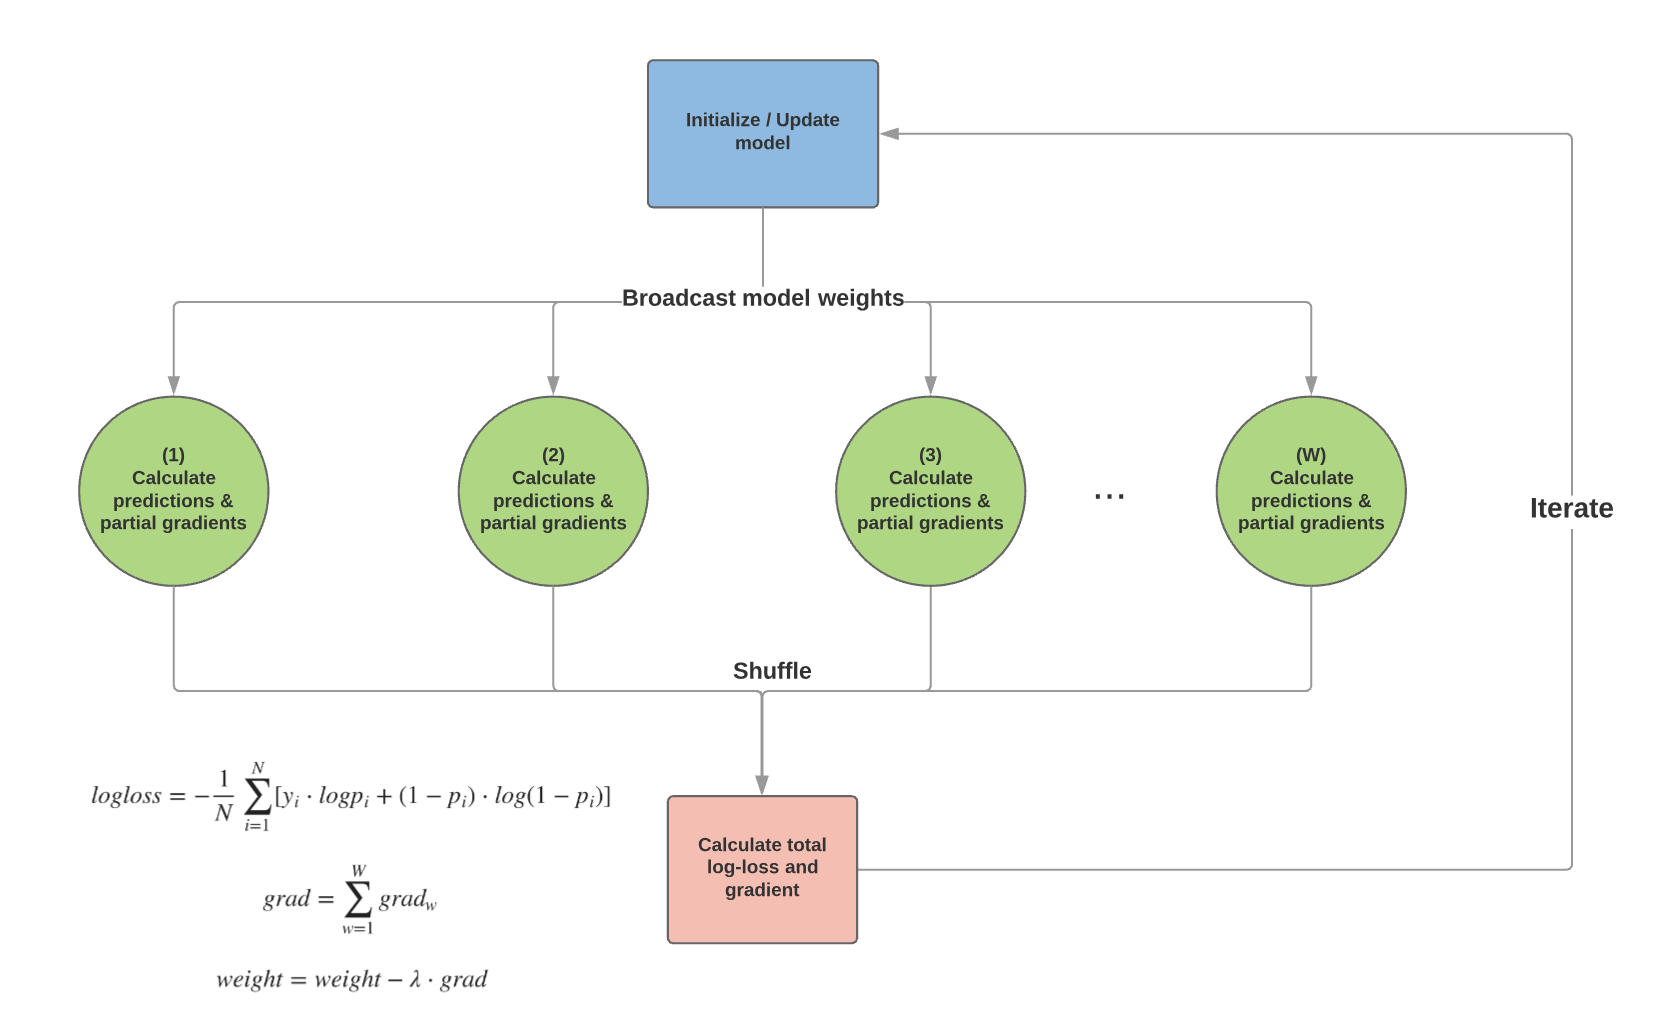
\includegraphics{FINAL/images/Data_Flow_Diagram.png}
\caption{FM factor}
\end{figure}

    \subsubsection{\texorpdfstring{\emph{Pre-Processing}}{Pre-Processing}}\label{pre-processing}

We begin by parsing our training data, appending the index number of the
raw column as a prefix to each value (e.g. categorical variable 12 with
value "online" becomes "c12\_online"). Similarly, we append "NA" to the
end of values that would otherwise be missing, and for numeric variables
we bucket them according to the raw distributions examined during our
exploratory analysis; this has the added benefit of limiting our feature
space and mitigating some risk of overfitting to the training data.

    \begin{Verbatim}[commandchars=\\\{\}]
{\color{incolor}In [{\color{incolor}9}]:} \PY{c+c1}{\PYZsh{} function to parse raw data and tag feature values with type and feature indices}
        \PY{k}{def} \PY{n+nf}{parseCV}\PY{p}{(}\PY{n}{line}\PY{p}{)}\PY{p}{:}
            \PY{l+s+sd}{\PYZdq{}\PYZdq{}\PYZdq{}}
        \PY{l+s+sd}{    Map text records to \PYZhy{}\PYZhy{}\PYZgt{} (label, features)}
        \PY{l+s+sd}{    Bucket (string) numeric features}
        \PY{l+s+sd}{    Add variable index prefix to feature values for binarization}
        \PY{l+s+sd}{    \PYZdq{}\PYZdq{}\PYZdq{}}
        
            \PY{c+c1}{\PYZsh{} start of categorical features}
            \PY{n}{col\PYZus{}start} \PY{o}{=} \PY{l+m+mi}{14}
            
            \PY{n}{raw\PYZus{}values} \PY{o}{=} \PY{n}{line}\PY{o}{.}\PY{n}{split}\PY{p}{(}\PY{l+s+s1}{\PYZsq{}}\PY{l+s+se}{\PYZbs{}t}\PY{l+s+s1}{\PYZsq{}}\PY{p}{)}
            \PY{n}{label} \PY{o}{=} \PY{n+nb}{int}\PY{p}{(}\PY{n}{raw\PYZus{}values}\PY{p}{[}\PY{l+m+mi}{0}\PY{p}{]}\PY{p}{)}
            
            \PY{c+c1}{\PYZsh{} parse numeric features}
            \PY{n}{numericals} \PY{o}{=} \PY{p}{[}\PY{p}{]}
            \PY{k}{for} \PY{n}{idx}\PY{p}{,} \PY{n}{value} \PY{o+ow}{in} \PY{n+nb}{enumerate}\PY{p}{(}\PY{n}{raw\PYZus{}values}\PY{p}{[}\PY{l+m+mi}{1}\PY{p}{:}\PY{n}{col\PYZus{}start}\PY{p}{]}\PY{p}{)}\PY{p}{:}
                \PY{k}{if} \PY{n}{value} \PY{o}{==} \PY{l+s+s1}{\PYZsq{}}\PY{l+s+s1}{\PYZsq{}}\PY{p}{:}
                    \PY{n}{append\PYZus{}val} \PY{o}{=} \PY{l+s+s1}{\PYZsq{}}\PY{l+s+s1}{NA}\PY{l+s+s1}{\PYZsq{}}
                \PY{k}{elif} \PY{n}{value} \PY{o}{==} \PY{l+s+s1}{\PYZsq{}}\PY{l+s+s1}{0}\PY{l+s+s1}{\PYZsq{}}\PY{p}{:}
                    \PY{n}{append\PYZus{}val} \PY{o}{=} \PY{l+s+s1}{\PYZsq{}}\PY{l+s+s1}{0}\PY{l+s+s1}{\PYZsq{}}
                \PY{k}{else}\PY{p}{:}
                    \PY{c+c1}{\PYZsh{} continues variables}
                    \PY{k}{if} \PY{n}{idx} \PY{o+ow}{in} \PY{p}{[}\PY{l+m+mi}{0}\PY{p}{,}\PY{l+m+mi}{3}\PY{p}{,}\PY{l+m+mi}{6}\PY{p}{,}\PY{l+m+mi}{7}\PY{p}{]}\PY{p}{:}
                        \PY{k}{if} \PY{n+nb}{float}\PY{p}{(}\PY{n}{value}\PY{p}{)}\PY{o}{\PYZlt{}}\PY{l+m+mi}{10}\PY{p}{:}
                            \PY{n}{append\PYZus{}val} \PY{o}{=} \PY{l+s+s1}{\PYZsq{}}\PY{l+s+s1}{\PYZlt{}10}\PY{l+s+s1}{\PYZsq{}}
                        \PY{k}{elif} \PY{n+nb}{float}\PY{p}{(}\PY{n}{value}\PY{p}{)}\PY{o}{\PYZlt{}}\PY{l+m+mi}{25}\PY{p}{:}
                            \PY{n}{append\PYZus{}val} \PY{o}{=} \PY{l+s+s1}{\PYZsq{}}\PY{l+s+s1}{\PYZlt{}25}\PY{l+s+s1}{\PYZsq{}}
                        \PY{k}{else}\PY{p}{:}
                            \PY{n}{append\PYZus{}val} \PY{o}{=} \PY{l+s+s1}{\PYZsq{}}\PY{l+s+s1}{\PYZgt{}25}\PY{l+s+s1}{\PYZsq{}}
                    \PY{k}{elif} \PY{n}{idx} \PY{o+ow}{in} \PY{p}{[}\PY{l+m+mi}{1}\PY{p}{,}\PY{l+m+mi}{2}\PY{p}{,}\PY{l+m+mi}{5}\PY{p}{]}\PY{p}{:}
                        \PY{k}{if} \PY{n+nb}{float}\PY{p}{(}\PY{n}{value}\PY{p}{)}\PY{o}{\PYZlt{}}\PY{l+m+mi}{100}\PY{p}{:}
                            \PY{n}{append\PYZus{}val} \PY{o}{=} \PY{l+s+s1}{\PYZsq{}}\PY{l+s+s1}{\PYZlt{}100}\PY{l+s+s1}{\PYZsq{}}
                        \PY{k}{else}\PY{p}{:}
                            \PY{n}{append\PYZus{}val} \PY{o}{=} \PY{l+s+s1}{\PYZsq{}}\PY{l+s+s1}{\PYZgt{}100}\PY{l+s+s1}{\PYZsq{}}
                    \PY{k}{elif} \PY{n}{idx}\PY{o}{==}\PY{l+m+mi}{4}\PY{p}{:}
                        \PY{k}{if} \PY{n+nb}{float}\PY{p}{(}\PY{n}{value}\PY{p}{)}\PY{o}{\PYZlt{}}\PY{l+m+mi}{10000}\PY{p}{:}
                            \PY{n}{append\PYZus{}val} \PY{o}{=} \PY{l+s+s1}{\PYZsq{}}\PY{l+s+s1}{\PYZlt{}10k}\PY{l+s+s1}{\PYZsq{}}
                        \PY{k}{elif} \PY{n+nb}{float}\PY{p}{(}\PY{n}{value}\PY{p}{)}\PY{o}{\PYZlt{}}\PY{l+m+mi}{50000}\PY{p}{:}
                            \PY{n}{append\PYZus{}val} \PY{o}{=} \PY{l+s+s1}{\PYZsq{}}\PY{l+s+s1}{\PYZlt{}50k}\PY{l+s+s1}{\PYZsq{}}
                        \PY{k}{else}\PY{p}{:}
                            \PY{n}{append\PYZus{}val} \PY{o}{=} \PY{l+s+s1}{\PYZsq{}}\PY{l+s+s1}{\PYZgt{}50k}\PY{l+s+s1}{\PYZsq{}}
                    \PY{k}{elif} \PY{n}{idx}\PY{o}{==}\PY{l+m+mi}{8}\PY{p}{:}
                        \PY{k}{if} \PY{n+nb}{float}\PY{p}{(}\PY{n}{value}\PY{p}{)}\PY{o}{\PYZlt{}}\PY{l+m+mi}{100}\PY{p}{:}
                            \PY{n}{append\PYZus{}val} \PY{o}{=} \PY{l+s+s1}{\PYZsq{}}\PY{l+s+s1}{\PYZlt{}100}\PY{l+s+s1}{\PYZsq{}}
                        \PY{k}{elif} \PY{n+nb}{float}\PY{p}{(}\PY{n}{value}\PY{p}{)}\PY{o}{\PYZlt{}}\PY{l+m+mi}{500}\PY{p}{:}
                            \PY{n}{append\PYZus{}val} \PY{o}{=} \PY{l+s+s1}{\PYZsq{}}\PY{l+s+s1}{\PYZlt{}500}\PY{l+s+s1}{\PYZsq{}}
                        \PY{k}{else}\PY{p}{:}
                            \PY{n}{append\PYZus{}val} \PY{o}{=} \PY{l+s+s1}{\PYZsq{}}\PY{l+s+s1}{\PYZgt{}500}\PY{l+s+s1}{\PYZsq{}}
                    \PY{k}{elif} \PY{n}{idx} \PY{o+ow}{in} \PY{p}{[}\PY{l+m+mi}{10}\PY{p}{,}\PY{l+m+mi}{11}\PY{p}{]}\PY{p}{:}
                        \PY{k}{if} \PY{n+nb}{float}\PY{p}{(}\PY{n}{value}\PY{p}{)}\PY{o}{\PYZlt{}}\PY{l+m+mi}{3}\PY{p}{:}
                            \PY{n}{append\PYZus{}val} \PY{o}{=} \PY{l+s+s1}{\PYZsq{}}\PY{l+s+s1}{\PYZlt{}3}\PY{l+s+s1}{\PYZsq{}}
                        \PY{k}{elif} \PY{n+nb}{float}\PY{p}{(}\PY{n}{value}\PY{p}{)}\PY{o}{\PYZlt{}}\PY{l+m+mi}{6}\PY{p}{:}
                            \PY{n}{append\PYZus{}val} \PY{o}{=} \PY{l+s+s1}{\PYZsq{}}\PY{l+s+s1}{\PYZlt{}6}\PY{l+s+s1}{\PYZsq{}}
                        \PY{k}{else}\PY{p}{:}
                            \PY{n}{append\PYZus{}val} \PY{o}{=} \PY{l+s+s1}{\PYZsq{}}\PY{l+s+s1}{\PYZgt{}6}\PY{l+s+s1}{\PYZsq{}}
                    \PY{k}{elif} \PY{n}{idx}\PY{o}{==}\PY{l+m+mi}{12}\PY{p}{:}
                        \PY{k}{if} \PY{n+nb}{float}\PY{p}{(}\PY{n}{value}\PY{p}{)}\PY{o}{\PYZlt{}}\PY{l+m+mi}{5}\PY{p}{:}
                            \PY{n}{append\PYZus{}val} \PY{o}{=} \PY{l+s+s1}{\PYZsq{}}\PY{l+s+s1}{\PYZlt{}5}\PY{l+s+s1}{\PYZsq{}}
                        \PY{k}{elif} \PY{n+nb}{float}\PY{p}{(}\PY{n}{value}\PY{p}{)}\PY{o}{\PYZlt{}}\PY{l+m+mi}{10}\PY{p}{:}
                            \PY{n}{append\PYZus{}val} \PY{o}{=} \PY{l+s+s1}{\PYZsq{}}\PY{l+s+s1}{\PYZlt{}10}\PY{l+s+s1}{\PYZsq{}}
                        \PY{k}{elif} \PY{n+nb}{float}\PY{p}{(}\PY{n}{value}\PY{p}{)}\PY{o}{\PYZlt{}}\PY{l+m+mi}{25}\PY{p}{:}
                            \PY{n}{append\PYZus{}val} \PY{o}{=} \PY{l+s+s1}{\PYZsq{}}\PY{l+s+s1}{\PYZlt{}25}\PY{l+s+s1}{\PYZsq{}}
                        \PY{k}{else}\PY{p}{:}
                            \PY{n}{append\PYZus{}val} \PY{o}{=} \PY{l+s+s1}{\PYZsq{}}\PY{l+s+s1}{\PYZgt{}25}\PY{l+s+s1}{\PYZsq{}}
                    \PY{c+c1}{\PYZsh{} ordinal/binary cases}
                    \PY{k}{else}\PY{p}{:}
                        \PY{n}{append\PYZus{}val} \PY{o}{=} \PY{n+nb}{str}\PY{p}{(}\PY{n}{value}\PY{p}{)}
                        
                \PY{n}{numericals}\PY{o}{.}\PY{n}{append}\PY{p}{(}\PY{l+s+s1}{\PYZsq{}}\PY{l+s+s1}{n}\PY{l+s+s1}{\PYZsq{}} \PY{o}{+} \PY{n+nb}{str}\PY{p}{(}\PY{n}{idx}\PY{p}{)} \PY{o}{+} \PY{l+s+s1}{\PYZsq{}}\PY{l+s+s1}{\PYZus{}}\PY{l+s+s1}{\PYZsq{}} \PY{o}{+} \PY{n}{append\PYZus{}val}\PY{p}{)}
                    
            \PY{c+c1}{\PYZsh{} parse categorical features}
            \PY{n}{categories} \PY{o}{=} \PY{p}{[}\PY{p}{]}
            \PY{k}{for} \PY{n}{idx}\PY{p}{,} \PY{n}{value} \PY{o+ow}{in} \PY{n+nb}{enumerate}\PY{p}{(}\PY{n}{raw\PYZus{}values}\PY{p}{[}\PY{n}{col\PYZus{}start}\PY{p}{:}\PY{p}{]}\PY{p}{)}\PY{p}{:}
                \PY{k}{if} \PY{n}{value} \PY{o}{==} \PY{l+s+s1}{\PYZsq{}}\PY{l+s+s1}{\PYZsq{}}\PY{p}{:}
                    \PY{n}{categories}\PY{o}{.}\PY{n}{append}\PY{p}{(}\PY{l+s+s1}{\PYZsq{}}\PY{l+s+s1}{c}\PY{l+s+s1}{\PYZsq{}}\PY{o}{+} \PY{n+nb}{str}\PY{p}{(}\PY{n}{idx}\PY{p}{)} \PY{o}{+} \PY{l+s+s1}{\PYZsq{}}\PY{l+s+s1}{\PYZus{}NA}\PY{l+s+s1}{\PYZsq{}}\PY{p}{)}
                \PY{k}{else}\PY{p}{:}
                    \PY{n}{categories}\PY{o}{.}\PY{n}{append}\PY{p}{(}\PY{l+s+s1}{\PYZsq{}}\PY{l+s+s1}{c}\PY{l+s+s1}{\PYZsq{}}\PY{o}{+} \PY{n+nb}{str}\PY{p}{(}\PY{n}{idx}\PY{p}{)} \PY{o}{+} \PY{l+s+s1}{\PYZsq{}}\PY{l+s+s1}{\PYZus{}}\PY{l+s+s1}{\PYZsq{}} \PY{o}{+} \PY{n+nb}{str}\PY{p}{(}\PY{n}{value}\PY{p}{)}\PY{p}{)}
        
            \PY{k}{return} \PY{n}{Row}\PY{p}{(}\PY{n}{label}\PY{o}{=}\PY{n}{label}\PY{p}{,} \PY{n}{raw}\PY{o}{=}\PY{n}{numericals} \PY{o}{+} \PY{n}{categories}\PY{p}{)}
\end{Verbatim}

    \begin{Verbatim}[commandchars=\\\{\}]
{\color{incolor}In [{\color{incolor}10}]:} \PY{c+c1}{\PYZsh{} call functions}
         \PY{n}{parsedDF} \PY{o}{=} \PY{n}{smallTrainRDD}\PY{o}{.}\PY{n}{map}\PY{p}{(}\PY{n}{parseCV}\PY{p}{)}\PY{o}{.}\PY{n}{toDF}\PY{p}{(}\PY{p}{)}
\end{Verbatim}

    \subsubsection{\texorpdfstring{\emph{One-Hot Encode All Features using
CountVectorizer for Sparse
Representation}}{One-Hot Encode All Features using CountVectorizer for Sparse Representation}}\label{one-hot-encode-all-features-using-countvectorizer-for-sparse-representation}

In order to efficiently move our data beginning in our driver program to
our worker nodes, and then perform computations on them, we need to
represent the features sparsely, or as vectors containing the indices of
the populated feature values. We can generate these features one time on
the master node by utilizing MLlib's CountVectorizer class to fit the
sparse representation and transform our string features as a new data
structure, which can later be added, or reduced following
parallelization.

    \begin{Verbatim}[commandchars=\\\{\}]
{\color{incolor}In [{\color{incolor}11}]:} \PY{c+c1}{\PYZsh{} function to one hot encode all features using a count vectorizer}
         \PY{k}{def} \PY{n+nf}{vectorizeCV}\PY{p}{(}\PY{n}{DF}\PY{p}{)}\PY{p}{:}
             
             \PY{n}{vectorizer} \PY{o}{=} \PY{n}{CountVectorizer}\PY{p}{(}\PY{p}{)}
             \PY{n}{cv} \PY{o}{=} \PY{n}{CountVectorizer}\PY{p}{(}\PY{n}{minDF}\PY{o}{=}\PY{l+m+mi}{1}\PY{p}{,} \PY{n}{inputCol}\PY{o}{=}\PY{l+s+s2}{\PYZdq{}}\PY{l+s+s2}{raw}\PY{l+s+s2}{\PYZdq{}}\PY{p}{,} \PY{n}{outputCol}\PY{o}{=}\PY{l+s+s2}{\PYZdq{}}\PY{l+s+s2}{features}\PY{l+s+s2}{\PYZdq{}}\PY{p}{)}
             
             \PY{n}{model} \PY{o}{=} \PY{n}{cv}\PY{o}{.}\PY{n}{fit}\PY{p}{(}\PY{n}{DF}\PY{p}{)}
             \PY{n}{result} \PY{o}{=} \PY{n}{model}\PY{o}{.}\PY{n}{transform}\PY{p}{(}\PY{n}{DF}\PY{p}{)}
             
             \PY{k}{return} \PY{n}{result}\PY{p}{,} \PY{n}{model}
\end{Verbatim}

    \begin{Verbatim}[commandchars=\\\{\}]
{\color{incolor}In [{\color{incolor}12}]:} \PY{n}{vectorizedDF}\PY{p}{,} \PY{n}{cvModel} \PY{o}{=} \PY{n}{vectorizeCV}\PY{p}{(}\PY{n}{parsedDF}\PY{p}{)}
         \PY{n}{vectorizedDF}\PY{o}{.}\PY{n}{show}\PY{p}{(}\PY{n}{truncate}\PY{o}{=}\PY{k+kc}{True}\PY{p}{)}
\end{Verbatim}

    \begin{Verbatim}[commandchars=\\\{\}]
+-----+--------------------+--------------------+
|label|                 raw|            features|
+-----+--------------------+--------------------+
|    0|[n0\_NA, n1\_<100, {\ldots}|(25739,[0,1,2,3,4{\ldots}|
|    0|[n0\_NA, n1\_<100, {\ldots}|(25739,[0,1,2,3,5{\ldots}|
|    1|[n0\_NA, n1\_<100, {\ldots}|(25739,[0,2,3,4,5{\ldots}|
|    0|[n0\_<10, n1\_<100,{\ldots}|(25739,[0,1,4,5,6{\ldots}|
|    1|[n0\_<10, n1\_<100,{\ldots}|(25739,[0,1,2,3,4{\ldots}|
|    1|[n0\_NA, n1\_<100, {\ldots}|(25739,[1,2,3,5,6{\ldots}|
|    0|[n0\_<10, n1\_<100,{\ldots}|(25739,[0,1,2,5,6{\ldots}|
|    0|[n0\_NA, n1\_<100, {\ldots}|(25739,[0,1,2,3,5{\ldots}|
|    0|[n0\_0, n1\_>100, n{\ldots}|(25739,[0,1,3,4,7{\ldots}|
|    0|[n0\_NA, n1\_0, n2\_{\ldots}|(25739,[0,2,3,4,8{\ldots}|
|    0|[n0\_0, n1\_<100, n{\ldots}|(25739,[0,1,2,4,5{\ldots}|
|    0|[n0\_<10, n1\_<100,{\ldots}|(25739,[0,1,2,4,5{\ldots}|
|    0|[n0\_NA, n1\_>100, {\ldots}|(25739,[1,2,3,6,7{\ldots}|
|    0|[n0\_0, n1\_>100, n{\ldots}|(25739,[0,1,4,6,8{\ldots}|
|    0|[n0\_0, n1\_<100, n{\ldots}|(25739,[0,1,2,5,6{\ldots}|
|    0|[n0\_NA, n1\_>100, {\ldots}|(25739,[1,2,3,6,7{\ldots}|
|    0|[n0\_NA, n1\_>100, {\ldots}|(25739,[0,1,2,3,7{\ldots}|
|    0|[n0\_NA, n1\_<100, {\ldots}|(25739,[1,2,3,5,6{\ldots}|
|    1|[n0\_<25, n1\_<100,{\ldots}|(25739,[0,1,2,3,4{\ldots}|
|    0|[n0\_NA, n1\_>100, {\ldots}|(25739,[0,1,2,3,7{\ldots}|
+-----+--------------------+--------------------+
only showing top 20 rows


    \end{Verbatim}

    \begin{Verbatim}[commandchars=\\\{\}]
{\color{incolor}In [{\color{incolor}13}]:} \PY{n}{vectorizedRDD} \PY{o}{=} \PY{n}{vectorizedDF}\PY{o}{.}\PY{n}{select}\PY{p}{(}\PY{p}{[}\PY{l+s+s1}{\PYZsq{}}\PY{l+s+s1}{label}\PY{l+s+s1}{\PYZsq{}}\PY{p}{,} \PY{l+s+s1}{\PYZsq{}}\PY{l+s+s1}{features}\PY{l+s+s1}{\PYZsq{}}\PY{p}{]}\PY{p}{)}\PY{o}{.}\PY{n}{rdd}\PY{o}{.}\PY{n}{cache}\PY{p}{(}\PY{p}{)}
\end{Verbatim}

    \begin{Verbatim}[commandchars=\\\{\}]
{\color{incolor}In [{\color{incolor}15}]:} \PY{n}{num\PYZus{}feats} \PY{o}{=} \PY{n}{vectorizedRDD}\PY{o}{.}\PY{n}{take}\PY{p}{(}\PY{l+m+mi}{1}\PY{p}{)}\PY{p}{[}\PY{l+m+mi}{0}\PY{p}{]}\PY{p}{[}\PY{l+m+mi}{1}\PY{p}{]}\PY{o}{.}\PY{n}{size}
         \PY{n}{percent\PYZus{}pos} \PY{o}{=} \PY{n}{vectorizedRDD}\PY{o}{.}\PY{n}{map}\PY{p}{(}\PY{k}{lambda} \PY{n}{x}\PY{p}{:} \PY{n}{x}\PY{p}{[}\PY{l+m+mi}{0}\PY{p}{]}\PY{p}{)}\PY{o}{.}\PY{n}{mean}\PY{p}{(}\PY{p}{)}
         
         \PY{n+nb}{print}\PY{p}{(}\PY{l+s+s2}{\PYZdq{}}\PY{l+s+s2}{Number of total expanded features:}\PY{l+s+s2}{\PYZdq{}}\PY{p}{,} \PY{n}{num\PYZus{}feats}\PY{p}{)}
         \PY{n+nb}{print}\PY{p}{(}\PY{l+s+s2}{\PYZdq{}}\PY{l+s+s2}{Relative frequency of positive class:}\PY{l+s+s2}{\PYZdq{}}\PY{p}{,} \PY{n}{percent\PYZus{}pos}\PY{p}{)}
\end{Verbatim}

    \begin{Verbatim}[commandchars=\\\{\}]
Number of total expanded features: 25739
Relative frequency of positive class: 0.25949084412684253

    \end{Verbatim}

    \subsection{\texorpdfstring{\emph{Predicting the Outcome and Estimating
Gradients}}{Predicting the Outcome and Estimating Gradients}}\label{predicting-the-outcome-and-estimating-gradients}

Next, with our improved data structure and our model equation discussed
in section 2., we can strategically perform computations such as
dot-products \emph{only on the populated feature values and the
corresponding elements of our parameter vector and matrix}, i.e. only
for those weight vector indices that correspond to our sparse feature
indices. Where our data only have an average on the order of 30
populated feature values per row, this is a fractional amount of
computation compared to the entire feature set or parameter matrix size.

    \begin{Verbatim}[commandchars=\\\{\}]
{\color{incolor}In [{\color{incolor}17}]:} \PY{k}{def} \PY{n+nf}{predictGrad}\PY{p}{(}\PY{n}{pair}\PY{p}{,} \PY{n}{k\PYZus{}br}\PY{p}{,} \PY{n}{b\PYZus{}br}\PY{p}{,} \PY{n}{w\PYZus{}br}\PY{p}{,} \PY{n}{V\PYZus{}br}\PY{p}{)}\PY{p}{:}
             \PY{l+s+sd}{\PYZdq{}\PYZdq{}\PYZdq{}}
         \PY{l+s+sd}{        Compute the predicted probability for average loss AND return the gradients}
         \PY{l+s+sd}{        Args:}
         \PY{l+s+sd}{            pair \PYZhy{} records are in (label, sparse feature set) format}
         \PY{l+s+sd}{        Broadcast:}
         \PY{l+s+sd}{            b \PYZhy{} bias term (scalar)}
         \PY{l+s+sd}{            w \PYZhy{} linear weight vector (array)}
         \PY{l+s+sd}{            k \PYZhy{} number of factors (def=2)}
         \PY{l+s+sd}{            V \PYZhy{} factor matrix of size (d dimensions, k=2 factors)}
         \PY{l+s+sd}{        Returns:}
         \PY{l+s+sd}{            predRDD \PYZhy{} pair of ([label, predicted probability], [set of weight vectors in csr\PYZus{}matrix format])}
         \PY{l+s+sd}{    \PYZdq{}\PYZdq{}\PYZdq{}}
             
             \PY{n}{label} \PY{o}{=} \PY{n}{pair}\PY{p}{[}\PY{l+m+mi}{0}\PY{p}{]}
             \PY{n}{feats} \PY{o}{=} \PY{n}{pair}\PY{p}{[}\PY{l+m+mi}{1}\PY{p}{]}
             
             \PY{c+c1}{\PYZsh{} start with linear weight dot product}
             \PY{n}{linear\PYZus{}sum} \PY{o}{=} \PY{n}{np}\PY{o}{.}\PY{n}{dot}\PY{p}{(}\PY{n}{w\PYZus{}br}\PY{o}{.}\PY{n}{value}\PY{p}{[}\PY{l+m+mi}{0}\PY{p}{]}\PY{p}{[}\PY{n}{feats}\PY{o}{.}\PY{n}{indices}\PY{p}{]}\PY{p}{,} \PY{n}{feats}\PY{o}{.}\PY{n}{values}\PY{p}{)}
         
             \PY{c+c1}{\PYZsh{} factor matrix interaction sum}
             \PY{n}{factor\PYZus{}sum} \PY{o}{=} \PY{l+m+mf}{0.0}
             \PY{n}{lh\PYZus{}factor} \PY{o}{=} \PY{p}{[}\PY{l+m+mf}{0.0}\PY{p}{]}\PY{o}{*}\PY{n}{k\PYZus{}br}\PY{o}{.}\PY{n}{value}
             \PY{n}{rh\PYZus{}factor} \PY{o}{=} \PY{p}{[}\PY{l+m+mf}{0.0}\PY{p}{]}\PY{o}{*}\PY{n}{k\PYZus{}br}\PY{o}{.}\PY{n}{value}
             
             \PY{k}{for} \PY{n}{f} \PY{o+ow}{in} \PY{n+nb}{range}\PY{p}{(}\PY{l+m+mi}{0}\PY{p}{,} \PY{n}{k\PYZus{}br}\PY{o}{.}\PY{n}{value}\PY{p}{)}\PY{p}{:}
                 \PY{n}{lh\PYZus{}factor}\PY{p}{[}\PY{n}{f}\PY{p}{]} \PY{o}{=} \PY{n}{np}\PY{o}{.}\PY{n}{dot}\PY{p}{(}\PY{n}{V\PYZus{}br}\PY{o}{.}\PY{n}{value}\PY{p}{[}\PY{n}{f}\PY{p}{]}\PY{p}{[}\PY{n}{feats}\PY{o}{.}\PY{n}{indices}\PY{p}{]}\PY{p}{,} \PY{n}{feats}\PY{o}{.}\PY{n}{values}\PY{p}{)}  \PY{c+c1}{\PYZsh{}KEY\PYZhy{}\PYZhy{}this is used in v\PYZus{}grad matrix below}
                 \PY{n}{rh\PYZus{}factor}\PY{p}{[}\PY{n}{f}\PY{p}{]} \PY{o}{=} \PY{n}{np}\PY{o}{.}\PY{n}{dot}\PY{p}{(}\PY{n}{V\PYZus{}br}\PY{o}{.}\PY{n}{value}\PY{p}{[}\PY{n}{f}\PY{p}{]}\PY{p}{[}\PY{n}{feats}\PY{o}{.}\PY{n}{indices}\PY{p}{]}\PY{o}{*}\PY{o}{*}\PY{l+m+mi}{2}\PY{p}{,} \PY{n}{feats}\PY{o}{.}\PY{n}{values}\PY{o}{*}\PY{o}{*}\PY{l+m+mi}{2}\PY{p}{)}
                 \PY{n}{factor\PYZus{}sum} \PY{o}{+}\PY{o}{=} \PY{p}{(}\PY{n}{lh\PYZus{}factor}\PY{p}{[}\PY{n}{f}\PY{p}{]}\PY{o}{*}\PY{o}{*}\PY{l+m+mi}{2} \PY{o}{\PYZhy{}} \PY{n}{rh\PYZus{}factor}\PY{p}{[}\PY{n}{f}\PY{p}{]}\PY{p}{)}
             \PY{n}{factor\PYZus{}sum} \PY{o}{=} \PY{l+m+mf}{0.5} \PY{o}{*} \PY{n}{factor\PYZus{}sum}
             
             \PY{n}{y\PYZus{}hat} \PY{o}{=} \PY{n}{b\PYZus{}br}\PY{o}{.}\PY{n}{value} \PY{o}{+} \PY{n}{linear\PYZus{}sum} \PY{o}{+} \PY{n}{factor\PYZus{}sum}    \PY{c+c1}{\PYZsh{}full model equation}
             
             \PY{n}{prob} \PY{o}{=} \PY{l+m+mf}{1.0} \PY{o}{/} \PY{p}{(}\PY{l+m+mi}{1} \PY{o}{+} \PY{n}{np}\PY{o}{.}\PY{n}{exp}\PY{p}{(}\PY{o}{\PYZhy{}}\PY{n}{y\PYZus{}hat}\PY{p}{)}\PY{p}{)}  \PY{c+c1}{\PYZsh{}logit transformation}
             
             \PY{c+c1}{\PYZsh{}compute Gradients}
             \PY{n}{b\PYZus{}grad} \PY{o}{=} \PY{n}{prob} \PY{o}{\PYZhy{}} \PY{n}{label}    \PY{c+c1}{\PYZsh{} bias term}
             
             \PY{c+c1}{\PYZsh{}linear term    }
             \PY{n}{w\PYZus{}grad} \PY{o}{=} \PY{n}{csr\PYZus{}matrix}\PY{p}{(}\PY{p}{(}\PY{n}{b\PYZus{}grad}\PY{o}{*}\PY{n}{feats}\PY{o}{.}\PY{n}{values}\PY{p}{,} \PY{p}{(}\PY{n}{np}\PY{o}{.}\PY{n}{zeros}\PY{p}{(}\PY{n}{feats}\PY{o}{.}\PY{n}{indices}\PY{o}{.}\PY{n}{size}\PY{p}{)}\PY{p}{,} \PY{n}{feats}\PY{o}{.}\PY{n}{indices}\PY{p}{)}\PY{p}{)}\PY{p}{,} \PY{n}{shape}\PY{o}{=}\PY{p}{(}\PY{l+m+mi}{1}\PY{p}{,} \PY{n}{w\PYZus{}br}\PY{o}{.}\PY{n}{value}\PY{o}{.}\PY{n}{shape}\PY{p}{[}\PY{l+m+mi}{1}\PY{p}{]}\PY{p}{)}\PY{p}{)}
             
             \PY{c+c1}{\PYZsh{}factor matrix (d*k)}
             \PY{n}{v\PYZus{}data} \PY{o}{=} \PY{n}{np}\PY{o}{.}\PY{n}{array}\PY{p}{(}\PY{p}{[}\PY{p}{]}\PY{p}{,} \PY{n}{dtype}\PY{o}{=}\PY{n}{np}\PY{o}{.}\PY{n}{float32}\PY{p}{)}
             \PY{n}{v\PYZus{}rows} \PY{o}{=} \PY{n}{np}\PY{o}{.}\PY{n}{array}\PY{p}{(}\PY{p}{[}\PY{p}{]}\PY{p}{,} \PY{n}{dtype}\PY{o}{=}\PY{n+nb}{int}\PY{p}{)}
             \PY{n}{v\PYZus{}cols} \PY{o}{=} \PY{n}{np}\PY{o}{.}\PY{n}{array}\PY{p}{(}\PY{p}{[}\PY{p}{]}\PY{p}{,} \PY{n}{dtype}\PY{o}{=}\PY{n+nb}{int}\PY{p}{)}
             \PY{k}{for} \PY{n}{i} \PY{o+ow}{in} \PY{n+nb}{range}\PY{p}{(}\PY{l+m+mi}{0}\PY{p}{,} \PY{n}{k\PYZus{}br}\PY{o}{.}\PY{n}{value}\PY{p}{)}\PY{p}{:}
                 \PY{n}{v\PYZus{}data} \PY{o}{=} \PY{n}{np}\PY{o}{.}\PY{n}{append}\PY{p}{(}\PY{n}{v\PYZus{}data}\PY{p}{,} \PY{n}{b\PYZus{}grad}\PY{o}{*}\PY{p}{(}\PY{n}{lh\PYZus{}factor}\PY{p}{[}\PY{n}{i}\PY{p}{]}\PY{o}{*}\PY{n}{feats}\PY{o}{.}\PY{n}{values} \PY{o}{\PYZhy{}} \PY{n}{np}\PY{o}{.}\PY{n}{multiply}\PY{p}{(}\PY{n}{V\PYZus{}br}\PY{o}{.}\PY{n}{value}\PY{p}{[}\PY{n}{i}\PY{p}{]}\PY{p}{[}\PY{n}{feats}\PY{o}{.}\PY{n}{indices}\PY{p}{]}\PY{p}{,} \PY{n}{feats}\PY{o}{.}\PY{n}{values}\PY{o}{*}\PY{o}{*}\PY{l+m+mi}{2}\PY{p}{)}\PY{p}{)}\PY{p}{)}
                 \PY{n}{v\PYZus{}rows} \PY{o}{=} \PY{n}{np}\PY{o}{.}\PY{n}{append}\PY{p}{(}\PY{n}{v\PYZus{}rows}\PY{p}{,} \PY{p}{[}\PY{n}{i}\PY{p}{]}\PY{o}{*}\PY{n}{feats}\PY{o}{.}\PY{n}{indices}\PY{o}{.}\PY{n}{size}\PY{p}{)}
                 \PY{n}{v\PYZus{}cols} \PY{o}{=} \PY{n}{np}\PY{o}{.}\PY{n}{append}\PY{p}{(}\PY{n}{v\PYZus{}cols}\PY{p}{,} \PY{n}{feats}\PY{o}{.}\PY{n}{indices}\PY{p}{)}
             \PY{n}{v\PYZus{}grad} \PY{o}{=} \PY{n}{csr\PYZus{}matrix}\PY{p}{(}\PY{p}{(}\PY{n}{v\PYZus{}data}\PY{p}{,} \PY{p}{(}\PY{n}{v\PYZus{}rows}\PY{p}{,} \PY{n}{v\PYZus{}cols}\PY{p}{)}\PY{p}{)}\PY{p}{,} \PY{n}{shape}\PY{o}{=}\PY{p}{(}\PY{n}{k\PYZus{}br}\PY{o}{.}\PY{n}{value}\PY{p}{,} \PY{n}{V\PYZus{}br}\PY{o}{.}\PY{n}{value}\PY{o}{.}\PY{n}{shape}\PY{p}{[}\PY{l+m+mi}{1}\PY{p}{]}\PY{p}{)}\PY{p}{)}
             
             \PY{k}{return} \PY{p}{(}\PY{p}{[}\PY{n}{label}\PY{p}{,} \PY{n}{prob}\PY{p}{]}\PY{p}{,} \PY{p}{[}\PY{n}{b\PYZus{}grad}\PY{p}{,} \PY{n}{w\PYZus{}grad}\PY{p}{,} \PY{n}{v\PYZus{}grad}\PY{p}{]}\PY{p}{)}
\end{Verbatim}

    At each step, we calculate our (negative) log-loss for each observation,
which will give us a sense of on average how close our predicted
probabilities are to their true outcome value (0 or 1).

    \begin{Verbatim}[commandchars=\\\{\}]
{\color{incolor}In [{\color{incolor}18}]:} \PY{k}{def} \PY{n+nf}{logLoss}\PY{p}{(}\PY{n}{pair}\PY{p}{)}\PY{p}{:}
             \PY{l+s+sd}{\PYZdq{}\PYZdq{}\PYZdq{}parallelize log\PYZhy{}loss calculation}
         \PY{l+s+sd}{        argument: ([label, prob], [b\PYZus{}grad, w\PYZus{}grad, v\PYZus{}grad])}
         \PY{l+s+sd}{        out: \PYZhy{}(log\PYZhy{}loss)}
         \PY{l+s+sd}{    \PYZdq{}\PYZdq{}\PYZdq{}}
             \PY{n}{y} \PY{o}{=} \PY{n}{pair}\PY{p}{[}\PY{l+m+mi}{0}\PY{p}{]}\PY{p}{[}\PY{l+m+mi}{1}\PY{p}{]}
             
             \PY{n}{eps} \PY{o}{=} \PY{l+m+mf}{1.0e\PYZhy{}16}
             \PY{k}{if} \PY{n}{pair}\PY{p}{[}\PY{l+m+mi}{0}\PY{p}{]}\PY{p}{[}\PY{l+m+mi}{1}\PY{p}{]} \PY{o}{==} \PY{l+m+mi}{0}\PY{p}{:}
                 \PY{n}{y\PYZus{}hat} \PY{o}{=} \PY{n}{eps}
             \PY{k}{elif} \PY{n}{pair}\PY{p}{[}\PY{l+m+mi}{0}\PY{p}{]}\PY{p}{[}\PY{l+m+mi}{1}\PY{p}{]} \PY{o}{==} \PY{l+m+mi}{1}\PY{p}{:}
                 \PY{n}{y\PYZus{}hat} \PY{o}{=} \PY{l+m+mi}{1}\PY{o}{\PYZhy{}}\PY{n}{eps}
             \PY{k}{else}\PY{p}{:}
                 \PY{n}{y\PYZus{}hat} \PY{o}{=} \PY{n}{pair}\PY{p}{[}\PY{l+m+mi}{0}\PY{p}{]}\PY{p}{[}\PY{l+m+mi}{1}\PY{p}{]}
             
             \PY{k}{return} \PY{o}{\PYZhy{}}\PY{p}{(}\PY{n}{y} \PY{o}{*} \PY{n}{np}\PY{o}{.}\PY{n}{log}\PY{p}{(}\PY{n}{y\PYZus{}hat}\PY{p}{)} \PY{o}{+} \PY{p}{(}\PY{l+m+mi}{1}\PY{o}{\PYZhy{}}\PY{n}{y}\PY{p}{)} \PY{o}{*} \PY{n}{np}\PY{o}{.}\PY{n}{log}\PY{p}{(}\PY{l+m+mi}{1}\PY{o}{\PYZhy{}}\PY{n}{y\PYZus{}hat}\PY{p}{)}\PY{p}{)}
\end{Verbatim}

    Where the probability, gradient and log-loss can all be calculated in
parallel, we will then need to shuffle our observations back together
and reduce our newly-estimated gradients, which conveniently can be
efficiently added even in sparse vector representation.

    \begin{Verbatim}[commandchars=\\\{\}]
{\color{incolor}In [{\color{incolor} }]:} \PY{k}{def} \PY{n+nf}{reduceFct}\PY{p}{(}\PY{n}{x}\PY{p}{,} \PY{n}{y}\PY{p}{)}\PY{p}{:}
            \PY{l+s+sd}{\PYZdq{}\PYZdq{}\PYZdq{}function for aggregating bias and weight matrices}
        \PY{l+s+sd}{        arguments: ([label, pred], [bias, weight, V matrix])}
        \PY{l+s+sd}{        out:       [sum bias b, sum weight w, sum matrix V]}
        \PY{l+s+sd}{    \PYZdq{}\PYZdq{}\PYZdq{}}
            \PY{n}{b} \PY{o}{=} \PY{n}{x}\PY{p}{[}\PY{l+m+mi}{0}\PY{p}{]} \PY{o}{+} \PY{n}{y}\PY{p}{[}\PY{l+m+mi}{0}\PY{p}{]}
            \PY{n}{w} \PY{o}{=} \PY{n}{x}\PY{p}{[}\PY{l+m+mi}{1}\PY{p}{]} \PY{o}{+} \PY{n}{y}\PY{p}{[}\PY{l+m+mi}{1}\PY{p}{]}
            \PY{n}{V} \PY{o}{=} \PY{n}{x}\PY{p}{[}\PY{l+m+mi}{2}\PY{p}{]} \PY{o}{+} \PY{n}{y}\PY{p}{[}\PY{l+m+mi}{2}\PY{p}{]}
            \PY{k}{return} \PY{p}{[}\PY{n}{b}\PY{p}{,} \PY{n}{w}\PY{p}{,} \PY{n}{V}\PY{p}{]}
\end{Verbatim}

    \subsubsection{\texorpdfstring{\emph{Model
Training}}{Model Training}}\label{model-training}

Now that we have our key map and reduce functions, we can iteratively
estimate our gradients and update our weight parameter estimates until
we achieve diminishing returns to our average log-loss. To do this,
however, we will need to broadcast our weight data structures to each
node, as well as keep our primary RDD containing features and labels
cached in worker memory, in order to minimize shuffling; however, given
the size of our weight vectors and full dataset, this will be
memory-intensive and ultimately require computation on a cluster.

    \begin{Verbatim}[commandchars=\\\{\}]
{\color{incolor}In [{\color{incolor}20}]:} \PY{k}{def} \PY{n+nf}{iterateSGD}\PY{p}{(}\PY{n}{dataRDD}\PY{p}{,} \PY{n}{k}\PY{p}{,} \PY{n}{bInit}\PY{p}{,} \PY{n}{wInit}\PY{p}{,} \PY{n}{vInit}\PY{p}{,} \PY{n}{nIter} \PY{o}{=} \PY{l+m+mi}{2}\PY{p}{,} \PY{n}{learningRate} \PY{o}{=} \PY{l+m+mf}{0.1}\PY{p}{,} \PY{n}{useReg} \PY{o}{=} \PY{k+kc}{False}\PY{p}{,} \PY{n}{regParam} \PY{o}{=} \PY{l+m+mf}{0.001}\PY{p}{)}\PY{p}{:}
         
             \PY{n}{k\PYZus{}br} \PY{o}{=} \PY{n}{sc}\PY{o}{.}\PY{n}{broadcast}\PY{p}{(}\PY{n}{k}\PY{p}{)}    
             \PY{n}{b\PYZus{}br} \PY{o}{=} \PY{n}{sc}\PY{o}{.}\PY{n}{broadcast}\PY{p}{(}\PY{n}{bInit}\PY{p}{)}
             \PY{n}{w\PYZus{}br} \PY{o}{=} \PY{n}{sc}\PY{o}{.}\PY{n}{broadcast}\PY{p}{(}\PY{n}{wInit}\PY{p}{)}
             \PY{n}{V\PYZus{}br} \PY{o}{=} \PY{n}{sc}\PY{o}{.}\PY{n}{broadcast}\PY{p}{(}\PY{n}{vInit}\PY{p}{)}
         
             \PY{n}{losses} \PY{o}{=} \PY{p}{[}\PY{p}{]}
             \PY{n}{N} \PY{o}{=} \PY{n}{dataRDD}\PY{o}{.}\PY{n}{count}\PY{p}{(}\PY{p}{)}
         
             \PY{k}{for} \PY{n}{i} \PY{o+ow}{in} \PY{n+nb}{range}\PY{p}{(}\PY{l+m+mi}{0}\PY{p}{,} \PY{n}{nIter}\PY{p}{)}\PY{p}{:}
                 \PY{n+nb}{print}\PY{p}{(}\PY{l+s+s1}{\PYZsq{}}\PY{l+s+s1}{\PYZhy{}}\PY{l+s+s1}{\PYZsq{}} \PY{o}{*} \PY{l+m+mi}{25} \PY{o}{+} \PY{l+s+s1}{\PYZsq{}}\PY{l+s+s1}{Iteration }\PY{l+s+s1}{\PYZsq{}} \PY{o}{+} \PY{n+nb}{str}\PY{p}{(}\PY{n}{i}\PY{o}{+}\PY{l+m+mi}{1}\PY{p}{)} \PY{o}{+} \PY{l+s+s1}{\PYZsq{}}\PY{l+s+s1}{\PYZhy{}}\PY{l+s+s1}{\PYZsq{}} \PY{o}{*} \PY{l+m+mi}{25}\PY{p}{)}
                 \PY{n}{predRDD} \PY{o}{=} \PY{n}{dataRDD}\PY{o}{.}\PY{n}{map}\PY{p}{(}\PY{k}{lambda} \PY{n}{x}\PY{p}{:} \PY{n}{predictGrad}\PY{p}{(}\PY{n}{x}\PY{p}{,} \PY{n}{k\PYZus{}br}\PY{p}{,} \PY{n}{b\PYZus{}br}\PY{p}{,} \PY{n}{w\PYZus{}br}\PY{p}{,} \PY{n}{V\PYZus{}br}\PY{p}{)}\PY{p}{)}\PY{o}{.}\PY{n}{cache}\PY{p}{(}\PY{p}{)}
                 
                 \PY{n}{loss} \PY{o}{=} \PY{n}{predRDD}\PY{o}{.}\PY{n}{map}\PY{p}{(}\PY{n}{logLoss}\PY{p}{)}\PY{o}{.}\PY{n}{reduce}\PY{p}{(}\PY{k}{lambda} \PY{n}{a}\PY{p}{,}\PY{n}{b}\PY{p}{:} \PY{n}{a}\PY{o}{+}\PY{n}{b}\PY{p}{)}\PY{o}{/}\PY{n}{N} \PY{o}{+} \PYZbs{}
                         \PY{n+nb}{int}\PY{p}{(}\PY{n}{useReg}\PY{p}{)}\PY{o}{*}\PY{p}{(}\PY{n}{regParam}\PY{o}{/}\PY{l+m+mi}{2}\PY{p}{)}\PY{o}{*}\PY{p}{(}\PY{n}{np}\PY{o}{.}\PY{n}{linalg}\PY{o}{.}\PY{n}{norm}\PY{p}{(}\PY{n}{w\PYZus{}br}\PY{o}{.}\PY{n}{value}\PY{p}{)}\PY{o}{*}\PY{o}{*}\PY{l+m+mi}{2} \PY{o}{+} \PY{n}{np}\PY{o}{.}\PY{n}{linalg}\PY{o}{.}\PY{n}{norm}\PY{p}{(}\PY{n}{V\PYZus{}br}\PY{o}{.}\PY{n}{value}\PY{p}{)}\PY{o}{*}\PY{o}{*}\PY{l+m+mi}{2}\PY{p}{)}
                 \PY{n}{losses}\PY{o}{.}\PY{n}{append}\PY{p}{(}\PY{n}{loss}\PY{p}{)}
                 \PY{n+nb}{print}\PY{p}{(}\PY{n}{f}\PY{l+s+s1}{\PYZsq{}}\PY{l+s+s1}{Current log\PYZhy{}loss: }\PY{l+s+si}{\PYZob{}loss\PYZcb{}}\PY{l+s+s1}{\PYZsq{}}\PY{p}{)}
                 
                 \PY{c+c1}{\PYZsh{} reduce step}
                 \PY{n}{gradRDD} \PY{o}{=} \PY{n}{predRDD}\PY{o}{.}\PY{n}{values}\PY{p}{(}\PY{p}{)}\PY{o}{.}\PY{n}{reduce}\PY{p}{(}\PY{n}{reduceFct}\PY{p}{)}
                 \PY{n}{bGrad} \PY{o}{=} \PY{n}{gradRDD}\PY{p}{[}\PY{l+m+mi}{0}\PY{p}{]}\PY{o}{/}\PY{n}{N}
                 \PY{n}{wGrad} \PY{o}{=} \PY{n}{gradRDD}\PY{p}{[}\PY{l+m+mi}{1}\PY{p}{]}\PY{o}{/}\PY{n}{N}
                 \PY{n}{vGrad} \PY{o}{=} \PY{n}{gradRDD}\PY{p}{[}\PY{l+m+mi}{2}\PY{p}{]}\PY{o}{/}\PY{n}{N}
         
                 \PY{n+nb}{print}\PY{p}{(}\PY{n}{f}\PY{l+s+s2}{\PYZdq{}}\PY{l+s+s2}{Bias: }\PY{l+s+si}{\PYZob{}bGrad\PYZcb{}}\PY{l+s+s2}{\PYZdq{}}\PY{p}{)}
                 \PY{n+nb}{print}\PY{p}{(}\PY{n}{f}\PY{l+s+s2}{\PYZdq{}}\PY{l+s+s2}{wGrad shape: }\PY{l+s+si}{\PYZob{}wGrad.shape\PYZcb{}}\PY{l+s+s2}{\PYZdq{}}\PY{p}{)}
                 \PY{n+nb}{print}\PY{p}{(}\PY{n}{f}\PY{l+s+s2}{\PYZdq{}}\PY{l+s+s2}{vGrad shape: }\PY{l+s+si}{\PYZob{}vGrad.shape\PYZcb{}}\PY{l+s+s2}{\PYZdq{}}\PY{p}{)}
         
                 \PY{c+c1}{\PYZsh{}\PYZsh{}\PYZsh{}\PYZsh{}\PYZsh{}\PYZsh{}\PYZsh{}\PYZsh{}\PYZsh{}\PYZsh{}\PYZsh{}\PYZsh{}\PYZsh{}\PYZsh{} update weights \PYZsh{}\PYZsh{}\PYZsh{}\PYZsh{}\PYZsh{}\PYZsh{}\PYZsh{}\PYZsh{}\PYZsh{}\PYZsh{}\PYZsh{}\PYZsh{}\PYZsh{}\PYZsh{}}
                 \PY{c+c1}{\PYZsh{} first, unpersist broadcasts}
                 \PY{n}{predRDD}\PY{o}{.}\PY{n}{unpersist}\PY{p}{(}\PY{p}{)}
                 \PY{n}{b\PYZus{}br}\PY{o}{.}\PY{n}{unpersist}\PY{p}{(}\PY{p}{)}
                 \PY{n}{w\PYZus{}br}\PY{o}{.}\PY{n}{unpersist}\PY{p}{(}\PY{p}{)}
                 \PY{n}{V\PYZus{}br}\PY{o}{.}\PY{n}{unpersist}\PY{p}{(}\PY{p}{)}
         
                 \PY{c+c1}{\PYZsh{} update and re\PYZhy{}broadcast}
                 \PY{n}{b\PYZus{}br} \PY{o}{=} \PY{n}{sc}\PY{o}{.}\PY{n}{broadcast}\PY{p}{(}\PY{n}{b\PYZus{}br}\PY{o}{.}\PY{n}{value} \PY{o}{\PYZhy{}} \PY{n}{learningRate} \PY{o}{*} \PY{n}{bGrad}\PY{p}{)}
                 \PY{n}{w\PYZus{}br} \PY{o}{=} \PY{n}{sc}\PY{o}{.}\PY{n}{broadcast}\PY{p}{(}\PY{n}{w\PYZus{}br}\PY{o}{.}\PY{n}{value} \PY{o}{\PYZhy{}} \PY{n}{learningRate} \PY{o}{*} \PY{p}{(}\PY{n}{wGrad}\PY{o}{.}\PY{n}{toarray}\PY{p}{(}\PY{p}{)}\PY{o}{+}\PY{n+nb}{int}\PY{p}{(}\PY{n}{useReg}\PY{p}{)}\PY{o}{*}\PY{n}{regParam}\PY{o}{*}\PY{n}{np}\PY{o}{.}\PY{n}{linalg}\PY{o}{.}\PY{n}{norm}\PY{p}{(}\PY{n}{w\PYZus{}br}\PY{o}{.}\PY{n}{value}\PY{p}{)}\PY{p}{)}\PY{p}{)}
                 \PY{n}{V\PYZus{}br} \PY{o}{=} \PY{n}{sc}\PY{o}{.}\PY{n}{broadcast}\PY{p}{(}\PY{n}{V\PYZus{}br}\PY{o}{.}\PY{n}{value} \PY{o}{\PYZhy{}} \PY{n}{learningRate} \PY{o}{*} \PY{p}{(}\PY{n}{vGrad}\PY{o}{.}\PY{n}{toarray}\PY{p}{(}\PY{p}{)}\PY{o}{+}\PY{n+nb}{int}\PY{p}{(}\PY{n}{useReg}\PY{p}{)}\PY{o}{*}\PY{n}{regParam}\PY{o}{*}\PY{n}{np}\PY{o}{.}\PY{n}{linalg}\PY{o}{.}\PY{n}{norm}\PY{p}{(}\PY{n}{V\PYZus{}br}\PY{o}{.}\PY{n}{value}\PY{p}{)}\PY{p}{)}\PY{p}{)}
                 
             \PY{k}{return} \PY{n}{losses}\PY{p}{,} \PY{n}{b\PYZus{}br}\PY{p}{,} \PY{n}{w\PYZus{}br}\PY{p}{,} \PY{n}{V\PYZus{}br}
\end{Verbatim}

    Below is again a sample of the data but run in a scaled manner, where
model parameters are initialized and broadcast, the training loop is set
to a fixed number of iterations, and there is no regularization. Here,
\(k\) is the order of variable interactions we wish the model to
consider, which is a tunable parameter, where the run-time is a function
of \(k\); a lower \(k\) may obscure possible interactions, but in a
sparse setting greatly reduces the likelihood of the model overfitting.
This model can accomodate L2 regularization, where the penalty is a
function of lambda and the magnitude of our weight vectors; however,
preliminary testing showed that this penalty did not help performance on
the validation set where our \(k\) is already conservative, and was thus
excluded from the full run. We also note that including the L2
regularization computation did not seem to substantially increase
runtime.

    \begin{Verbatim}[commandchars=\\\{\}]
{\color{incolor}In [{\color{incolor}25}]:} \PY{c+c1}{\PYZsh{} initialize weights}
         \PY{n}{np}\PY{o}{.}\PY{n}{random}\PY{o}{.}\PY{n}{seed}\PY{p}{(}\PY{l+m+mi}{24}\PY{p}{)}
         \PY{n}{k} \PY{o}{=} \PY{l+m+mi}{2}
         \PY{n}{b} \PY{o}{=} \PY{l+m+mf}{0.0}
         \PY{n}{w} \PY{o}{=} \PY{n}{np}\PY{o}{.}\PY{n}{random}\PY{o}{.}\PY{n}{normal}\PY{p}{(}\PY{l+m+mf}{0.0}\PY{p}{,} \PY{l+m+mf}{0.02}\PY{p}{,} \PY{p}{(}\PY{l+m+mi}{1}\PY{p}{,} \PY{n}{num\PYZus{}feats}\PY{p}{)}\PY{p}{)}
         \PY{n}{V} \PY{o}{=} \PY{n}{np}\PY{o}{.}\PY{n}{random}\PY{o}{.}\PY{n}{normal}\PY{p}{(}\PY{l+m+mf}{0.0}\PY{p}{,} \PY{l+m+mf}{0.02}\PY{p}{,} \PY{p}{(}\PY{n}{k}\PY{p}{,} \PY{n}{num\PYZus{}feats}\PY{p}{)}\PY{p}{)}
         
         \PY{c+c1}{\PYZsh{} train sample model}
         \PY{n}{nIter} \PY{o}{=} \PY{l+m+mi}{10}
         \PY{n}{start} \PY{o}{=} \PY{n}{time}\PY{o}{.}\PY{n}{time}\PY{p}{(}\PY{p}{)}
         \PY{n}{losses}\PY{p}{,} \PY{n}{b\PYZus{}br}\PY{p}{,} \PY{n}{w\PYZus{}br}\PY{p}{,} \PY{n}{V\PYZus{}br} \PY{o}{=} \PY{n}{iterateSGD}\PY{p}{(}\PY{n}{vectorizedRDD}\PY{p}{,} \PY{n}{k}\PY{p}{,} \PY{n}{b}\PY{p}{,} \PY{n}{w}\PY{p}{,} \PY{n}{V}\PY{p}{,} \PY{n}{nIter}\PY{p}{)}
         \PY{n+nb}{print}\PY{p}{(}\PY{n}{f}\PY{l+s+s1}{\PYZsq{}}\PY{l+s+s1}{Performed }\PY{l+s+si}{\PYZob{}nIter\PYZcb{}}\PY{l+s+s1}{ iterations in }\PY{l+s+s1}{\PYZob{}}\PY{l+s+s1}{time.time() \PYZhy{} start\PYZcb{} seconds}\PY{l+s+s1}{\PYZsq{}}\PY{p}{)}
\end{Verbatim}

    \begin{Verbatim}[commandchars=\\\{\}]
-------------------------Iteration 1-------------------------
Current log-loss: 0.6912273009710425
Bias: 0.25436576408125167
wGrad shape: (1, 25739)
vGrad shape: (2, 25739)
-------------------------Iteration 2-------------------------
Current log-loss: 0.6851338435935052
Bias: 0.18375948102046125
wGrad shape: (1, 25739)
vGrad shape: (2, 25739)
-------------------------Iteration 3-------------------------
Current log-loss: 0.6687666092907115
Bias: 0.13441639427762675
wGrad shape: (1, 25739)
vGrad shape: (2, 25739)
-------------------------Iteration 4-------------------------
Current log-loss: 0.6512226506271765
Bias: 0.09992019607042654
wGrad shape: (1, 25739)
vGrad shape: (2, 25739)
-------------------------Iteration 5-------------------------
Current log-loss: 0.6356066208636996
Bias: 0.07543655596140342
wGrad shape: (1, 25739)
vGrad shape: (2, 25739)
-------------------------Iteration 6-------------------------
Current log-loss: 0.622623423080275
Bias: 0.05774713712429709
wGrad shape: (1, 25739)
vGrad shape: (2, 25739)
-------------------------Iteration 7-------------------------
Current log-loss: 0.6121412223222497
Bias: 0.04475662909105663
wGrad shape: (1, 25739)
vGrad shape: (2, 25739)
-------------------------Iteration 8-------------------------
Current log-loss: 0.6037891852325022
Bias: 0.03508540602284818
wGrad shape: (1, 25739)
vGrad shape: (2, 25739)
-------------------------Iteration 9-------------------------
Current log-loss: 0.5971714200881342
Bias: 0.02780504477504894
wGrad shape: (1, 25739)
vGrad shape: (2, 25739)
-------------------------Iteration 10-------------------------
Current log-loss: 0.5919359790827723
Bias: 0.022275786379377382
wGrad shape: (1, 25739)
vGrad shape: (2, 25739)
Performed 10 iterations in 404.480101108551 seconds

    \end{Verbatim}

    \begin{Verbatim}[commandchars=\\\{\}]
{\color{incolor}In [{\color{incolor}27}]:} \PY{n}{fig}\PY{p}{,} \PY{n}{ax} \PY{o}{=} \PY{n}{plt}\PY{o}{.}\PY{n}{subplots}\PY{p}{(}\PY{l+m+mi}{1}\PY{p}{,}\PY{l+m+mi}{1}\PY{p}{,}\PY{n}{figsize} \PY{o}{=} \PY{p}{(}\PY{l+m+mi}{16}\PY{p}{,}\PY{l+m+mi}{8}\PY{p}{)}\PY{p}{)}
         \PY{n}{x} \PY{o}{=} \PY{n+nb}{list}\PY{p}{(}\PY{n+nb}{range}\PY{p}{(}\PY{l+m+mi}{1}\PY{p}{,} \PY{n+nb}{len}\PY{p}{(}\PY{n}{losses}\PY{p}{)}\PY{o}{+}\PY{l+m+mi}{1}\PY{p}{)}\PY{p}{)}
         \PY{n}{ax}\PY{o}{.}\PY{n}{plot}\PY{p}{(}\PY{n}{x}\PY{p}{,} \PY{n}{losses}\PY{p}{,} \PY{l+s+s1}{\PYZsq{}}\PY{l+s+s1}{k\PYZhy{}\PYZhy{}}\PY{l+s+s1}{\PYZsq{}}\PY{p}{,} \PY{n}{label}\PY{o}{=}\PY{l+s+s1}{\PYZsq{}}\PY{l+s+s1}{Training Loss}\PY{l+s+s1}{\PYZsq{}}\PY{p}{)}
         \PY{n}{ax}\PY{o}{.}\PY{n}{legend}\PY{p}{(}\PY{n}{loc}\PY{o}{=}\PY{l+s+s1}{\PYZsq{}}\PY{l+s+s1}{upper right}\PY{l+s+s1}{\PYZsq{}}\PY{p}{,} \PY{n}{fontsize}\PY{o}{=}\PY{l+s+s1}{\PYZsq{}}\PY{l+s+s1}{x\PYZhy{}large}\PY{l+s+s1}{\PYZsq{}}\PY{p}{)}
         \PY{n}{plt}\PY{o}{.}\PY{n}{xlabel}\PY{p}{(}\PY{l+s+s1}{\PYZsq{}}\PY{l+s+s1}{Number of Iterations}\PY{l+s+s1}{\PYZsq{}}\PY{p}{)}
         \PY{n}{plt}\PY{o}{.}\PY{n}{title}\PY{p}{(}\PY{l+s+s2}{\PYZdq{}}\PY{l+s+s2}{Log\PYZhy{}Loss}\PY{l+s+s2}{\PYZdq{}}\PY{p}{)}
         \PY{n}{plt}\PY{o}{.}\PY{n}{show}\PY{p}{(}\PY{p}{)}
\end{Verbatim}

    \begin{center}
    \adjustimage{max size={0.9\linewidth}{0.9\paperheight}}{output_107_0.png}
    \end{center}
    { \hspace*{\fill} \\}
    
    \subsection{\texorpdfstring{\emph{Sample Evaluation of Holdout
Development
Set}}{Sample Evaluation of Holdout Development Set}}\label{sample-evaluation-of-holdout-development-set}

To confirm that we are not overfitting our model to our sample training
set, we next calculate the log-loss on a holdout set of labeled data,
using the same CountVectorizer transformation and FM model equation to
estimate our \(\hat{p}\).

    \begin{Verbatim}[commandchars=\\\{\}]
{\color{incolor}In [{\color{incolor}28}]:} \PY{k}{def} \PY{n+nf}{predictProb}\PY{p}{(}\PY{n}{pair}\PY{p}{,} \PY{n}{k\PYZus{}br}\PY{p}{,} \PY{n}{b\PYZus{}br}\PY{p}{,} \PY{n}{w\PYZus{}br}\PY{p}{,} \PY{n}{V\PYZus{}br}\PY{p}{)}\PY{p}{:}
             \PY{l+s+sd}{\PYZdq{}\PYZdq{}\PYZdq{}}
         \PY{l+s+sd}{        Compute the predicted probability AND return the gradient (?)}
         \PY{l+s+sd}{        Args:}
         \PY{l+s+sd}{            pair \PYZhy{} records are in (label, sparse feature set) format}
         \PY{l+s+sd}{        Broadcast:}
         \PY{l+s+sd}{            b \PYZhy{} bias term (scalar)}
         \PY{l+s+sd}{            w \PYZhy{} linear weight vector (array)}
         \PY{l+s+sd}{            k \PYZhy{} number of factors (def=2)}
         \PY{l+s+sd}{            V \PYZhy{} factor matrix of size (d dimensions, k=2 factors)}
         \PY{l+s+sd}{        Returns:}
         \PY{l+s+sd}{            predRDD \PYZhy{} pair of (label, predicted probability)}
         \PY{l+s+sd}{    \PYZdq{}\PYZdq{}\PYZdq{}}
             
             \PY{n}{label} \PY{o}{=} \PY{n}{pair}\PY{p}{[}\PY{l+m+mi}{0}\PY{p}{]}
             \PY{n}{feats} \PY{o}{=} \PY{n}{pair}\PY{p}{[}\PY{l+m+mi}{1}\PY{p}{]}
             
             \PY{c+c1}{\PYZsh{} start with linear weight dot product}
             \PY{n}{linear\PYZus{}sum} \PY{o}{=} \PY{n}{np}\PY{o}{.}\PY{n}{dot}\PY{p}{(}\PY{n}{w\PYZus{}br}\PY{o}{.}\PY{n}{value}\PY{p}{[}\PY{l+m+mi}{0}\PY{p}{]}\PY{p}{[}\PY{n}{feats}\PY{o}{.}\PY{n}{indices}\PY{p}{]}\PY{p}{,} \PY{n}{feats}\PY{o}{.}\PY{n}{values}\PY{p}{)}
         
             \PY{c+c1}{\PYZsh{} factor matrix interaction sum}
             \PY{n}{factor\PYZus{}sum} \PY{o}{=} \PY{l+m+mf}{0.0}
             \PY{n}{lh\PYZus{}factor} \PY{o}{=} \PY{p}{[}\PY{l+m+mf}{0.0}\PY{p}{]}\PY{o}{*}\PY{n}{k\PYZus{}br}\PY{o}{.}\PY{n}{value}
             \PY{n}{rh\PYZus{}factor} \PY{o}{=} \PY{p}{[}\PY{l+m+mf}{0.0}\PY{p}{]}\PY{o}{*}\PY{n}{k\PYZus{}br}\PY{o}{.}\PY{n}{value}
             
             \PY{k}{for} \PY{n}{f} \PY{o+ow}{in} \PY{n+nb}{range}\PY{p}{(}\PY{l+m+mi}{0}\PY{p}{,} \PY{n}{k\PYZus{}br}\PY{o}{.}\PY{n}{value}\PY{p}{)}\PY{p}{:}
                 \PY{n}{lh\PYZus{}factor}\PY{p}{[}\PY{n}{f}\PY{p}{]} \PY{o}{=} \PY{n}{np}\PY{o}{.}\PY{n}{dot}\PY{p}{(}\PY{n}{V\PYZus{}br}\PY{o}{.}\PY{n}{value}\PY{p}{[}\PY{n}{f}\PY{p}{]}\PY{p}{[}\PY{n}{feats}\PY{o}{.}\PY{n}{indices}\PY{p}{]}\PY{p}{,} \PY{n}{feats}\PY{o}{.}\PY{n}{values}\PY{p}{)}
                 \PY{n}{rh\PYZus{}factor}\PY{p}{[}\PY{n}{f}\PY{p}{]} \PY{o}{=} \PY{n}{np}\PY{o}{.}\PY{n}{dot}\PY{p}{(}\PY{n}{V\PYZus{}br}\PY{o}{.}\PY{n}{value}\PY{p}{[}\PY{n}{f}\PY{p}{]}\PY{p}{[}\PY{n}{feats}\PY{o}{.}\PY{n}{indices}\PY{p}{]}\PY{o}{*}\PY{o}{*}\PY{l+m+mi}{2}\PY{p}{,} \PY{n}{feats}\PY{o}{.}\PY{n}{values}\PY{o}{*}\PY{o}{*}\PY{l+m+mi}{2}\PY{p}{)}
                 \PY{n}{factor\PYZus{}sum} \PY{o}{+}\PY{o}{=} \PY{p}{(}\PY{n}{lh\PYZus{}factor}\PY{p}{[}\PY{n}{f}\PY{p}{]}\PY{o}{*}\PY{o}{*}\PY{l+m+mi}{2} \PY{o}{\PYZhy{}} \PY{n}{rh\PYZus{}factor}\PY{p}{[}\PY{n}{f}\PY{p}{]}\PY{p}{)}
             \PY{n}{factor\PYZus{}sum} \PY{o}{=} \PY{l+m+mf}{0.5} \PY{o}{*} \PY{n}{factor\PYZus{}sum}
             
             \PY{n}{pre\PYZus{}prob} \PY{o}{=} \PY{n}{b\PYZus{}br}\PY{o}{.}\PY{n}{value} \PY{o}{+} \PY{n}{linear\PYZus{}sum} \PY{o}{+} \PY{n}{factor\PYZus{}sum}
             
             \PY{n}{prob} \PY{o}{=} \PY{l+m+mf}{1.0} \PY{o}{/} \PY{p}{(}\PY{l+m+mi}{1} \PY{o}{+} \PY{n}{np}\PY{o}{.}\PY{n}{exp}\PY{p}{(}\PY{o}{\PYZhy{}}\PY{n}{pre\PYZus{}prob}\PY{p}{)}\PY{p}{)}  \PY{c+c1}{\PYZsh{}logit transformation}
             
             \PY{k}{return} \PY{p}{(}\PY{n}{label}\PY{p}{,} \PY{n}{prob}\PY{p}{)}
\end{Verbatim}

    \begin{Verbatim}[commandchars=\\\{\}]
{\color{incolor}In [{\color{incolor}29}]:} \PY{k}{def} \PY{n+nf}{testLoss}\PY{p}{(}\PY{n}{pair}\PY{p}{)}\PY{p}{:}
             \PY{l+s+sd}{\PYZdq{}\PYZdq{}\PYZdq{}parallelize log loss}
         \PY{l+s+sd}{        input: (label, prob)}
         \PY{l+s+sd}{    \PYZdq{}\PYZdq{}\PYZdq{}}
             \PY{n}{y} \PY{o}{=} \PY{n}{pair}\PY{p}{[}\PY{l+m+mi}{0}\PY{p}{]}
             
             \PY{n}{eps} \PY{o}{=} \PY{l+m+mf}{1.0e\PYZhy{}16}
             \PY{k}{if} \PY{n}{pair}\PY{p}{[}\PY{l+m+mi}{1}\PY{p}{]} \PY{o}{==} \PY{l+m+mi}{0}\PY{p}{:}
                 \PY{n}{y\PYZus{}hat} \PY{o}{=} \PY{n}{eps}
             \PY{k}{elif} \PY{n}{pair}\PY{p}{[}\PY{l+m+mi}{1}\PY{p}{]} \PY{o}{==} \PY{l+m+mi}{1}\PY{p}{:}
                 \PY{n}{y\PYZus{}hat} \PY{o}{=} \PY{l+m+mi}{1}\PY{o}{\PYZhy{}}\PY{n}{eps}
             \PY{k}{else}\PY{p}{:}
                 \PY{n}{y\PYZus{}hat} \PY{o}{=} \PY{n}{pair}\PY{p}{[}\PY{l+m+mi}{1}\PY{p}{]}
             
             \PY{k}{return} \PY{o}{\PYZhy{}}\PY{p}{(}\PY{n}{y} \PY{o}{*} \PY{n}{np}\PY{o}{.}\PY{n}{log}\PY{p}{(}\PY{n}{y\PYZus{}hat}\PY{p}{)} \PY{o}{+} \PY{p}{(}\PY{l+m+mi}{1}\PY{o}{\PYZhy{}}\PY{n}{y}\PY{p}{)} \PY{o}{*} \PY{n}{np}\PY{o}{.}\PY{n}{log}\PY{p}{(}\PY{l+m+mi}{1}\PY{o}{\PYZhy{}}\PY{n}{y\PYZus{}hat}\PY{p}{)}\PY{p}{)}
\end{Verbatim}

    \begin{Verbatim}[commandchars=\\\{\}]
{\color{incolor}In [{\color{incolor}30}]:} \PY{n}{k\PYZus{}br} \PY{o}{=} \PY{n}{sc}\PY{o}{.}\PY{n}{broadcast}\PY{p}{(}\PY{n}{k}\PY{p}{)}
         
         \PY{n}{parsedTestDF} \PY{o}{=} \PY{n}{smallTestRDD}\PY{o}{.}\PY{n}{map}\PY{p}{(}\PY{n}{parseCV}\PY{p}{)}\PY{o}{.}\PY{n}{toDF}\PY{p}{(}\PY{p}{)}
         \PY{n}{vectorizedTestDF} \PY{o}{=} \PY{n}{cvModel}\PY{o}{.}\PY{n}{transform}\PY{p}{(}\PY{n}{parsedTestDF}\PY{p}{)}
         \PY{n}{testLoss} \PY{o}{=} \PY{n}{vectorizedTestDF}\PY{o}{.}\PY{n}{select}\PY{p}{(}\PY{p}{[}\PY{l+s+s1}{\PYZsq{}}\PY{l+s+s1}{label}\PY{l+s+s1}{\PYZsq{}}\PY{p}{,} \PY{l+s+s1}{\PYZsq{}}\PY{l+s+s1}{features}\PY{l+s+s1}{\PYZsq{}}\PY{p}{]}\PY{p}{)}\PY{o}{.}\PY{n}{rdd} \PYZbs{}
                                             \PY{o}{.}\PY{n}{map}\PY{p}{(}\PY{k}{lambda} \PY{n}{x}\PY{p}{:} \PY{n}{predictProb}\PY{p}{(}\PY{n}{x}\PY{p}{,} \PY{n}{k\PYZus{}br}\PY{p}{,} \PY{n}{b\PYZus{}br}\PY{p}{,} \PY{n}{w\PYZus{}br}\PY{p}{,} \PY{n}{V\PYZus{}br}\PY{p}{)}\PY{p}{)} \PYZbs{}
                                             \PY{o}{.}\PY{n}{map}\PY{p}{(}\PY{n}{testLoss}\PY{p}{)}\PY{o}{.}\PY{n}{mean}\PY{p}{(}\PY{p}{)}
         
         \PY{n+nb}{print}\PY{p}{(}\PY{l+s+s2}{\PYZdq{}}\PY{l+s+s2}{Log\PYZhy{}loss on the hold\PYZhy{}out development set is:}\PY{l+s+s2}{\PYZdq{}}\PY{p}{,} \PY{n}{testLoss}\PY{p}{)}
\end{Verbatim}

    \begin{Verbatim}[commandchars=\\\{\}]
Log-loss on the hold-out development set is: 0.5588072612641066

    \end{Verbatim}

    \subsection{\texorpdfstring{\emph{Full Model Training on GCP
Cluster}}{Full Model Training on GCP Cluster}}\label{full-model-training-on-gcp-cluster}

    The previous code was inserted into a pyspark file for submission to a
GCP dataproc cluster, named \texttt{fm\_on\_cluster.py}. We used helper
code provided by the instructors, \texttt{submit\_job\_to\_cluster.py},
to specify the cluster creation and submit the pyspark job, and we
additionally modified the code to allow the specification of different
machine types for the master and the workers.

The results shown below are for a dataproc training job using a random
sample of 80\% of the \texttt{training.txt} dataset over 25 learning
iterations, and evaluated on the remaining 20\% of held-out user
observations. This split contains close to 37 million training
observations (plus 7 million in the holdout set) and 262,000 binarized
features. Accordingly, our parameters are our scalar bias term
\texttt{b}, linear weight vector \(w\), and \(k=2\)-wide factor matrix
\textbf{V}.

    \begin{Verbatim}[commandchars=\\\{\}]
{\color{incolor}In [{\color{incolor}1}]:} \PY{n}{fullLoss\PYZus{}txt} \PY{o}{=} \PY{n+nb}{open}\PY{p}{(}\PY{l+s+s2}{\PYZdq{}}\PY{l+s+s2}{FINAL/results/results\PYZus{}train\PYZus{}loss.txt}\PY{l+s+s2}{\PYZdq{}}\PY{p}{,} \PY{l+s+s2}{\PYZdq{}}\PY{l+s+s2}{r}\PY{l+s+s2}{\PYZdq{}}\PY{p}{)}
        \PY{n}{fullLoss\PYZus{}list} \PY{o}{=} \PY{n}{fullLoss\PYZus{}txt}\PY{o}{.}\PY{n}{read}\PY{p}{(}\PY{p}{)}\PY{o}{.}\PY{n}{split}\PY{p}{(}\PY{l+s+s1}{\PYZsq{}}\PY{l+s+se}{\PYZbs{}t}\PY{l+s+s1}{\PYZsq{}}\PY{p}{)}
        \PY{n}{fullLoss} \PY{o}{=} \PY{p}{[}\PY{n+nb}{float}\PY{p}{(}\PY{n}{loss}\PY{p}{)} \PY{k}{for} \PY{n}{loss} \PY{o+ow}{in} \PY{n}{fullLoss\PYZus{}list}\PY{p}{[}\PY{p}{:}\PY{o}{\PYZhy{}}\PY{l+m+mi}{1}\PY{p}{]}\PY{p}{]}
\end{Verbatim}

    \begin{Verbatim}[commandchars=\\\{\}]
{\color{incolor}In [{\color{incolor}3}]:} \PY{n}{fig}\PY{p}{,} \PY{n}{ax} \PY{o}{=} \PY{n}{plt}\PY{o}{.}\PY{n}{subplots}\PY{p}{(}\PY{l+m+mi}{1}\PY{p}{,}\PY{l+m+mi}{1}\PY{p}{,}\PY{n}{figsize} \PY{o}{=} \PY{p}{(}\PY{l+m+mi}{12}\PY{p}{,}\PY{l+m+mi}{6}\PY{p}{)}\PY{p}{)}
        \PY{n}{x} \PY{o}{=} \PY{n+nb}{list}\PY{p}{(}\PY{n+nb}{range}\PY{p}{(}\PY{l+m+mi}{1}\PY{p}{,}\PY{n+nb}{len}\PY{p}{(}\PY{n}{fullLoss}\PY{p}{)}\PY{o}{+}\PY{l+m+mi}{1}\PY{p}{)}\PY{p}{)}
        \PY{n}{ax}\PY{o}{.}\PY{n}{plot}\PY{p}{(}\PY{n}{x}\PY{p}{,} \PY{n}{fullLoss}\PY{p}{,} \PY{l+s+s1}{\PYZsq{}}\PY{l+s+s1}{k\PYZhy{}\PYZhy{}}\PY{l+s+s1}{\PYZsq{}}\PY{p}{,} \PY{n}{label}\PY{o}{=}\PY{l+s+s1}{\PYZsq{}}\PY{l+s+s1}{Full Training Set (80}\PY{l+s+s1}{\PYZpc{}}\PY{l+s+s1}{) Loss}\PY{l+s+s1}{\PYZsq{}}\PY{p}{)}
        \PY{n}{ax}\PY{o}{.}\PY{n}{legend}\PY{p}{(}\PY{n}{loc}\PY{o}{=}\PY{l+s+s1}{\PYZsq{}}\PY{l+s+s1}{upper right}\PY{l+s+s1}{\PYZsq{}}\PY{p}{,} \PY{n}{fontsize}\PY{o}{=}\PY{l+s+s1}{\PYZsq{}}\PY{l+s+s1}{x\PYZhy{}large}\PY{l+s+s1}{\PYZsq{}}\PY{p}{)}
        \PY{n}{plt}\PY{o}{.}\PY{n}{xlabel}\PY{p}{(}\PY{l+s+s1}{\PYZsq{}}\PY{l+s+s1}{Number of Iterations}\PY{l+s+s1}{\PYZsq{}}\PY{p}{)}
        \PY{n}{plt}\PY{o}{.}\PY{n}{title}\PY{p}{(}\PY{l+s+s2}{\PYZdq{}}\PY{l+s+s2}{Log\PYZhy{}Loss}\PY{l+s+s2}{\PYZdq{}}\PY{p}{)}
        \PY{n}{plt}\PY{o}{.}\PY{n}{show}\PY{p}{(}\PY{p}{)}
\end{Verbatim}

    \begin{center}
    \adjustimage{max size={0.9\linewidth}{0.9\paperheight}}{output_115_0.png}
    \end{center}
    { \hspace*{\fill} \\}
    
    Over the first ten iterations, we see rapid improvement in our average
log-loss for our training set over the first ten iterations, with a
leveling out thereafter. On our holdout set, we estimate an average loss
on a similar order but slightly lower, which suggests our model could
benefit from generating additional features, as the current is underfit.

    \begin{Verbatim}[commandchars=\\\{\}]
{\color{incolor}In [{\color{incolor}4}]:} \PY{n}{testLoss\PYZus{}txt} \PY{o}{=} \PY{n+nb}{open}\PY{p}{(}\PY{l+s+s2}{\PYZdq{}}\PY{l+s+s2}{FINAL/results/results\PYZus{}test\PYZus{}loss.txt}\PY{l+s+s2}{\PYZdq{}}\PY{p}{,} \PY{l+s+s2}{\PYZdq{}}\PY{l+s+s2}{r}\PY{l+s+s2}{\PYZdq{}}\PY{p}{)}
        \PY{n}{testLoss} \PY{o}{=} \PY{n+nb}{float}\PY{p}{(}\PY{n}{testLoss\PYZus{}txt}\PY{o}{.}\PY{n}{read}\PY{p}{(}\PY{p}{)}\PY{p}{)}
        \PY{n+nb}{print}\PY{p}{(}\PY{l+s+s2}{\PYZdq{}}\PY{l+s+s2}{Final loss on our holdout data of the train.txt set:}\PY{l+s+s2}{\PYZdq{}}\PY{p}{,} \PY{n}{testLoss}\PY{p}{)}
\end{Verbatim}

    \begin{Verbatim}[commandchars=\\\{\}]
Final loss on our holdout data of the train.txt set: 0.548992525753779

    \end{Verbatim}

    \subsection{\texorpdfstring{\emph{Score Unlabeled Test
Data}}{Score Unlabeled Test Data}}\label{score-unlabeled-test-data}

As an extension of our holdout set accuracy evaluation, we score the
unlabeled \texttt{test.txt} data using the model trained on the cluster.
This requires again first transforming our raw features using the save
CV model:

    \begin{Verbatim}[commandchars=\\\{\}]
{\color{incolor}In [{\color{incolor}31}]:} \PY{n}{unlabeledRDD} \PY{o}{=} \PY{n}{sc}\PY{o}{.}\PY{n}{textFile}\PY{p}{(}\PY{l+s+s1}{\PYZsq{}}\PY{l+s+s1}{data/test.txt}\PY{l+s+s1}{\PYZsq{}}\PY{p}{)}
         \PY{n}{scoreTest} \PY{o}{=} \PY{l+m+mf}{0.001}
         \PY{n}{smallUnlabeledRDD} \PY{o}{=} \PY{n}{unlabeledRDD}\PY{o}{.}\PY{n}{sample}\PY{p}{(}\PY{k+kc}{False}\PY{p}{,} \PY{n}{scoreTest}\PY{p}{)}
\end{Verbatim}

    \begin{Verbatim}[commandchars=\\\{\}]
{\color{incolor}In [{\color{incolor}32}]:} \PY{n}{parsedUnlabeledDF} \PY{o}{=} \PY{n}{smallUnlabeledRDD}\PY{o}{.}\PY{n}{map}\PY{p}{(}\PY{k}{lambda} \PY{n}{x}\PY{p}{:} \PY{l+s+s2}{\PYZdq{}}\PY{l+s+s2}{0}\PY{l+s+se}{\PYZbs{}t}\PY{l+s+s2}{\PYZdq{}}\PY{o}{+}\PY{n}{x}\PY{p}{)}\PY{o}{.}\PY{n}{map}\PY{p}{(}\PY{n}{parseCV}\PY{p}{)}\PY{o}{.}\PY{n}{toDF}\PY{p}{(}\PY{p}{)}
         \PY{n}{vectorUnlabeledDF} \PY{o}{=} \PY{n}{cvModel}\PY{o}{.}\PY{n}{transform}\PY{p}{(}\PY{n}{parsedUnlabeledDF}\PY{p}{)}
         \PY{n}{vectorUnlabeledDF}\PY{o}{.}\PY{n}{show}\PY{p}{(}\PY{n}{truncate}\PY{o}{=}\PY{k+kc}{True}\PY{p}{)}
\end{Verbatim}

    \begin{Verbatim}[commandchars=\\\{\}]
+-----+--------------------+--------------------+
|label|                 raw|            features|
+-----+--------------------+--------------------+
|    0|[n0\_<10, n1\_<100,{\ldots}|(25739,[0,1,4,5,6{\ldots}|
|    0|[n0\_NA, n1\_<100, {\ldots}|(25739,[0,1,2,3,4{\ldots}|
|    0|[n0\_0, n1\_0, n2\_<{\ldots}|(25739,[0,1,2,3,4{\ldots}|
|    0|[n0\_NA, n1\_<100, {\ldots}|(25739,[3,5,6,8,1{\ldots}|
|    0|[n0\_0, n1\_<100, n{\ldots}|(25739,[0,1,2,3,4{\ldots}|
|    0|[n0\_<10, n1\_0, n2{\ldots}|(25739,[0,1,3,4,8{\ldots}|
|    0|[n0\_NA, n1\_<100, {\ldots}|(25739,[0,1,3,5,6{\ldots}|
|    0|[n0\_0, n1\_<100, n{\ldots}|(25739,[0,2,4,5,1{\ldots}|
|    0|[n0\_NA, n1\_<100, {\ldots}|(25739,[0,2,3,4,5{\ldots}|
|    0|[n0\_NA, n1\_>100, {\ldots}|(25739,[1,2,3,6,1{\ldots}|
|    0|[n0\_0, n1\_0, n2\_>{\ldots}|(25739,[0,1,4,6,9{\ldots}|
|    0|[n0\_<10, n1\_<100,{\ldots}|(25739,[0,1,2,3,4{\ldots}|
|    0|[n0\_NA, n1\_<100, {\ldots}|(25739,[1,2,5,6,7{\ldots}|
|    0|[n0\_NA, n1\_0, n2\_{\ldots}|(25739,[1,2,3,7,9{\ldots}|
|    0|[n0\_NA, n1\_<100, {\ldots}|(25739,[0,1,2,3,4{\ldots}|
|    0|[n0\_<10, n1\_<100,{\ldots}|(25739,[0,1,2,3,4{\ldots}|
|    0|[n0\_<25, n1\_<100,{\ldots}|(25739,[0,1,3,4,5{\ldots}|
|    0|[n0\_<10, n1\_<100,{\ldots}|(25739,[0,2,3,4,5{\ldots}|
|    0|[n0\_NA, n1\_<100, {\ldots}|(25739,[0,1,2,3,4{\ldots}|
|    0|[n0\_<10, n1\_0, n2{\ldots}|(25739,[0,1,2,4,7{\ldots}|
+-----+--------------------+--------------------+
only showing top 20 rows


    \end{Verbatim}

    Using our full model trained and validated with the labeled data on our
cluster, we evaluate the robustness of our model's scoring, given what
we know and expect about the distribution of our CTR outcome variable.

    \begin{Verbatim}[commandchars=\\\{\}]
{\color{incolor}In [{\color{incolor}6}]:} \PY{k+kn}{import} \PY{n+nn}{pandas} \PY{k}{as} \PY{n+nn}{pd}
        \PY{n}{unlabeledScores} \PY{o}{=} \PY{n}{pd}\PY{o}{.}\PY{n}{read\PYZus{}csv}\PY{p}{(}\PY{l+s+s2}{\PYZdq{}}\PY{l+s+s2}{FINAL/results/results\PYZus{}test\PYZus{}predictions.csv}\PY{l+s+s2}{\PYZdq{}}\PY{p}{,} \PY{n}{names} \PY{o}{=} \PY{p}{[}\PY{l+s+s2}{\PYZdq{}}\PY{l+s+s2}{One\PYZhy{}hot encoded features}\PY{l+s+s2}{\PYZdq{}}\PY{p}{,} \PY{l+s+s2}{\PYZdq{}}\PY{l+s+s2}{Score}\PY{l+s+s2}{\PYZdq{}}\PY{p}{]}\PY{p}{)}
        \PY{n}{unlabeledScores}\PY{o}{.}\PY{n}{head}\PY{p}{(}\PY{l+m+mi}{10}\PY{p}{)}
\end{Verbatim}

\begin{Verbatim}[commandchars=\\\{\}]
{\color{outcolor}Out[{\color{outcolor}6}]:}                             One-hot encoded features     Score
        0  ['n0\_<25', 'n1\_<100', 'n2\_<100', 'n3\_<10', 'n4{\ldots}  0.322991
        1  ['n0\_0', 'n1\_<100', 'n2\_<100', 'n3\_<25', 'n4\_<{\ldots}  0.240020
        2  ['n0\_NA', 'n1\_<100', 'n2\_<100', 'n3\_<25', 'n4\_{\ldots}  0.183301
        3  ['n0\_<10', 'n1\_<100', 'n2\_>100', 'n3\_NA', 'n4\_{\ldots}  0.240142
        4  ['n0\_NA', 'n1\_0', 'n2\_<100', 'n3\_<10', 'n4\_<10{\ldots}  0.205011
        5  ['n0\_0', 'n1\_<100', 'n2\_<100', 'n3\_>25', 'n4\_<{\ldots}  0.272889
        6  ['n0\_<10', 'n1\_<100', 'n2\_<100', 'n3\_<10', 'n4{\ldots}  0.279814
        7  ['n0\_<10', 'n1\_<100', 'n2\_<100', 'n3\_<10', 'n4{\ldots}  0.287328
        8  ['n0\_0', 'n1\_0', 'n2\_<100', 'n3\_NA', 'n4\_<50k'{\ldots}  0.231372
        9  ['n0\_<10', 'n1\_<100', 'n2\_<100', 'n3\_<10', 'n4{\ldots}  0.272297
\end{Verbatim}
            
    \begin{Verbatim}[commandchars=\\\{\}]
{\color{incolor}In [{\color{incolor}7}]:} \PY{n}{unlabeledScores}\PY{o}{.}\PY{n}{shape}
\end{Verbatim}

\begin{Verbatim}[commandchars=\\\{\}]
{\color{outcolor}Out[{\color{outcolor}7}]:} (60738, 2)
\end{Verbatim}
            
    Looking at a randomly drawn sample of roughly 60,000 user observations
from the unlabeled test set, we see a narrow distribution of predicted
probabilities centered around our mean training sample CTR. This
suggests that although our model improved in its log-loss after each
iteration, the trained model is lacking strong features and possibly
more latent factors that could represent additional interactions between
independent variables. There is a large opportunity for improvement
toward practical accuracy from additional feature engineering.

    \begin{Verbatim}[commandchars=\\\{\}]
{\color{incolor}In [{\color{incolor}9}]:} \PY{n}{plt}\PY{o}{.}\PY{n}{hist}\PY{p}{(}\PY{n}{unlabeledScores}\PY{p}{[}\PY{l+s+s2}{\PYZdq{}}\PY{l+s+s2}{Score}\PY{l+s+s2}{\PYZdq{}}\PY{p}{]}\PY{p}{,} \PY{n+nb}{range}\PY{o}{=}\PY{p}{(}\PY{l+m+mi}{0}\PY{p}{,}\PY{l+m+mi}{1}\PY{p}{)}\PY{p}{,} \PY{n}{bins}\PY{o}{=}\PY{l+m+mi}{40}\PY{p}{)}
        \PY{n}{plt}\PY{o}{.}\PY{n}{xlabel}\PY{p}{(}\PY{l+s+s1}{\PYZsq{}}\PY{l+s+s1}{Estimated Probability}\PY{l+s+s1}{\PYZsq{}}\PY{p}{)}
        \PY{n}{plt}\PY{o}{.}\PY{n}{ylabel}\PY{p}{(}\PY{l+s+s1}{\PYZsq{}}\PY{l+s+s1}{Frequency}\PY{l+s+s1}{\PYZsq{}}\PY{p}{)}
        \PY{n}{plt}\PY{o}{.}\PY{n}{title}\PY{p}{(}\PY{l+s+s1}{\PYZsq{}}\PY{l+s+s1}{Scoring of Unlabeled Test Data}\PY{l+s+s1}{\PYZsq{}}\PY{p}{)}
        \PY{n}{plt}\PY{o}{.}\PY{n}{show}\PY{p}{(}\PY{p}{)}
\end{Verbatim}

    \begin{center}
    \adjustimage{max size={0.9\linewidth}{0.9\paperheight}}{output_125_0.png}
    \end{center}
    { \hspace*{\fill} \\}
    
    \subsection{\texorpdfstring{\emph{Training Time at
Scale}}{Training Time at Scale}}\label{training-time-at-scale}

Evaluating our run-time using different training sample proportions, we
see strong evidence that we have achieved roughly linear run-time purely
as a function of the fraction of training data used when using a
parameter of \(k=2\). This is encouraging because even as the size of
our one-hot encoded feature space is also growing (and thus the number
of our order=2 feature interactions), we are not led to an exponential
increase in run-time. This suggests that we have achieved scalability
under the wide, sparse feature problem, and if we were to increase the
number of latent factors \(k\), we would expect only an increase in
run-time by a factor of each additional \(k\); for example, if we went
from two to four latent factors, we expect twice as many computations
per row in our mapper, and thus a doubling of run-time. Note that the
regression line shows that the training time is not strictly linear, but
is clearly not growing exponentially. We suspect that there may be
additional overhead (e.g., time required to broadcast larger and larger
model weights) that are increasing the training time with more and more
data.

    \begin{figure}
\centering
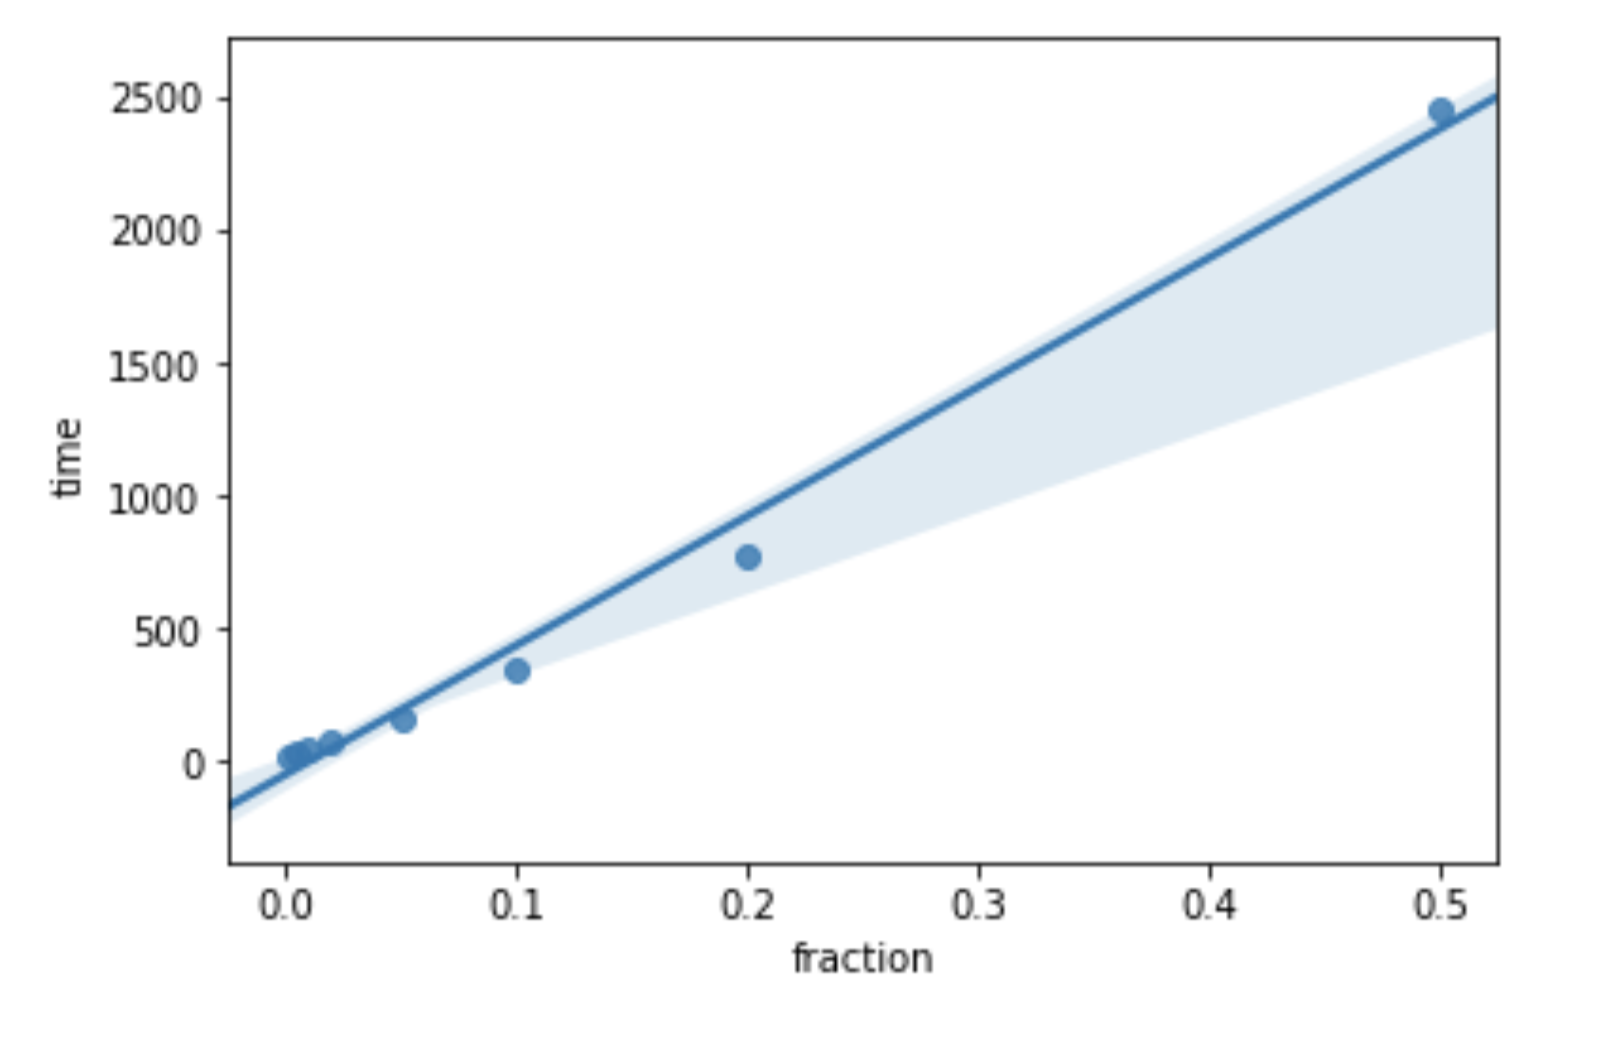
\includegraphics{FINAL/images/Training_Time.png}
\caption{FM factor}
\end{figure}

    

    \section{5. Key Concepts of Machine Learning at
Scale}\label{key-concepts-of-machine-learning-at-scale}

The direction of this project was determined by several core concepts
from this course:

\begin{itemize}
\tightlist
\item
  functional programming / higher order functions / map reduce paradigm
\item
  associative / commutative operations
\item
  broadcasting / caching
\item
  sparse representation (pairs vs stripes)
\item
  one-hot encoding / vector embeddings
\item
  normalization
\end{itemize}

The model presented here takes advantage of the fact that gradient
descent is parallelizable. Calculating the gradient for each example in
the training data depends only on the broadcast model weights and factor
matrix, and not on information captured by other examples. The final
gradient is an average of these estimates across all examples. Since the
first step of taking this average is to sum all gradient calculations
together, the preceding individual gradient calculations are not
impacted by the order in which gradients are calculated (making them
commutative operations) and do not depend on which partitions calculate
which gradients (associative), making this task embarrassingly parallel.
To take advantage of parallelization, we utilize the functional
programming paradigm of map-reduce and Spark, such as using the
higher-order \texttt{map} function of RDDs to estimate the new gradient
of each example. From a technical standpoint, the function depends only
on the example and the broadcast model variables passed to it, although
in our case those broadcast variables are sizeable data structures. But
we do note that from a conceptual standpoint, usage of the broadcast
variables is a departure from the 'statelessness' of the functional
programming paradigm. Distributing these parallel computations across a
cluster allows true gradient descent to be accomplished in significantly
reduced execution time, thus eliminating the need to approximate
gradients with an approach such as stochastic gradient descent.

As mentioned previously, broadcasting the weight matrix and factor
matrix allows every executor in the cluster to perform the same gradient
calculation with its partition of data. However, both full model
parameters have hundreds of thousands of elements, so broadcasting these
was a concern in terms of both data transfer and memory usage of the
executors. Since high memory usage of these broadcasts was anticipated,
caching of RDDs was only used tactfully in order to minimize memory
usage. Two RDDs are accessed multiple times during training iterations
(such as the one-hot encoded \texttt{vectorizedRDD}) and are therefore
cached in order to avoid their recalculation. This avoids duplication of
RDD calculations, and is used in accordance with
\texttt{RDD.unpersist()} where appropriate to release these RDDs and
broadcast variables from memory when they are no longer needed. Careful
caching and unpersisting permitted the high memory demand of large
broadcasts while eliminating unnecessary calculations.

The model makes heavy use of vector embeddings. The original dataset
started very close to a ``stripes'' format-\/- the label (outcome) of an
example is accompanied by an array of features associated with that
label. \texttt{CountVectorizer} is used to convert this dense
representation into a sparse vector representation of the data, in which
all feature values become one-hot encoded. The columns represent each
unique feature value, and each row is a web user, where an entry in the
feature matrix takes value 1 if that example contains the feature in
that column, and 0 if not. Given the enormous number of categorical
values throughout the data, as well as the fact that their meanings
(i.e. ordering) are unknown, the one-hot encoding allows a numerical
representation of the data that can be efficiently processed by many
machine learning algorithms (e.g. similarity between examples can be
calculated). The factorization machines method also creates a vector
representation of the strength of each variable (\(w\)), as well as the
single and pairwise interactions between features (\(V\), when \(k=2\)).
Because of the extremely large but sparse feature space, the matrix
representation of interactions \(V\), while large and typically a
significant drag on computation time, is only selectively used to
perform operations with the \emph{populated feature values} of \(x\). As
a result, we gain substantial computational benefit from representing
our features with compressed sparse row vectors, which also have the
benefit of being reducible when determining each training iteration's
gradient.

Early on in the process of transforming the data, we attempted to
normalize the values to the (0, 1) range to expedite convergence on
gradient descent and regularization (which are both more efficient when
features are on the same scale). In order to handle the missing values,
the columns needed to be transposed to keys, bringing the data
representation back to a `pairs' approach, and we considered this to be
too inefficient for processing. Furthermore, the EDA showed that a) most
numerical variables were highly skewed towards zero across a large range
(values close to zero would be hard to discern when scaling down), and
b) a log transform could misconstrue the way zero values are
represented. The numerical data was instead bucketed into categories,
which simplified the one-hot encoded representation of the data. One-hot
encoding the buckets of numerical variables was considered a sufficient
representation of those variables that allows proper gradient descent
and regularization while also simplifying the dataset.

Understanding the above concepts is crucial to determining the data
representations, model choices, and algorithm design that result in a
machine learning application that can scale well. The model created
effectively analyzes a week's worth of data in about a day, meaning it
could be put into production for Criteo's regular use with a computation
cost of only one hundred dollars a week or just over five thousand
dollars each year. A few future improvements to increase the model
accuracy could include parameter tuning the size of the interaction
matrix, normalizing the numeric features, and leveraging libraries such
as Glint to more efficiently deal with sharing and updating large model
weights and vectors across many worker nodes.


    % Add a bibliography block to the postdoc
    
    
    
    \end{document}
